% =====================================================================
%  END-OF-STUDIES PROJECT — MAIN DOCUMENT (corrected preamble)
%  Adem Mrabet — Polytech Intl — Data Science — 2025/2026
%
%  WHAT CHANGED vs your version (all verified by compiling):
%   1. fncychap now loads BEFORE minitoc  (minitoc requires this order)
%   2. titlesec REMOVED — minitoc declares it incompatible
%   3. minitoc loaded ONCE, \dominitoc called ONCE
%   4. stray \minitoc removed from the preamble (it belongs after \chapter)
%   5. graphicx no longer uses [pdftex] — clashed with tikz
%   6. hyperref moved to the end, where it belongs
% =====================================================================

\documentclass[12pt,a4paper]{report}

\usepackage[top=1.9cm, bottom=2.5cm, left=2.5cm, right=2cm]{geometry}

% ---------------------------------------------------------------
% ENCODING / LANGUAGE / FONT
% ---------------------------------------------------------------
\usepackage[utf8]{inputenc}
\usepackage[T1]{fontenc}
\usepackage[english]{babel}
\usepackage{newtxtext,newtxmath}
\usepackage{longtable}% Times New Roman

% ---------------------------------------------------------------
% CHAPTER STYLE
% fncychap MUST be loaded BEFORE minitoc, or minitoc warns W0086
% and the \chapter command ends up altered underneath it.
% ---------------------------------------------------------------
\usepackage[Rejne]{fncychap}
\ChTitleVar{\Huge\sffamily\bfseries}
\setlength{\headheight}{15pt}

% ---------------------------------------------------------------
% MINITOC — per-chapter mini tables of contents
% Loaded ONCE. \dominitoc called ONCE, after all its settings.
% DO NOT load titlesec anywhere in this file: minitoc reports it
% as incompatible (warning W0099) and chapter handling breaks.
% ---------------------------------------------------------------
\usepackage{minitoc}
\setcounter{minitocdepth}{2}
\renewcommand{\mtctitle}{Contents}
\mtcsetrules{minitoc}{off}
\setlength{\mtcindent}{0pt}
\dominitoc

% ---------------------------------------------------------------
% COLOUR / TABLES / GRAPHICS
% ---------------------------------------------------------------
\usepackage[table,xcdraw]{xcolor}
\definecolor{myblue}{HTML}{00723F}
\usepackage{colortbl}
\usepackage{multirow}
\usepackage{hhline}
\usepackage{array}
\usepackage{float}
\usepackage{graphicx}          % NO [pdftex] — it clashes with tikz
\usepackage{pdflscape}
\usepackage{adjustbox}
\usepackage{changepage}
\usepackage{tikz}
\def\checkmark{\tikz\fill[scale=0.4](0,.35) -- (.25,0) -- (1,.7) -- (.25,.15) -- cycle;}

% ---------------------------------------------------------------
% MATHS / SYMBOLS / SPACING
% ---------------------------------------------------------------
\usepackage{amsmath}
\usepackage{amssymb}
\usepackage{textcomp}
\usepackage{ragged2e}
\usepackage{setspace}
\onehalfspacing

% ---------------------------------------------------------------
% BIBLIOGRAPHY / ACRONYMS / APPENDIX
% ---------------------------------------------------------------
\usepackage[square, numbers]{natbib}
\usepackage[withpage]{acronym}
\usepackage[toc,page]{appendix}
\usepackage{subcaption}

% ---------------------------------------------------------------
% NUMBERING DEPTH  (gives you 1.1.1.1 and lists it in the contents)
% ---------------------------------------------------------------
\setcounter{secnumdepth}{3}
\setcounter{tocdepth}{3}

% ---------------------------------------------------------------
% HEADERS AND FOOTERS
% ---------------------------------------------------------------
\usepackage{fancyhdr}
\pagestyle{fancy}
\fancyhead[L]{}
\fancyhead[C]{}
\fancyhead[R]{\nouppercase{\rightmark}}
\fancyfoot[L]{}
\fancyfoot[C]{}
\fancyfoot[R]{\textbf{\thepage}}

% ---------------------------------------------------------------
% CROSS-REFERENCES AND LINKS — hyperref goes LAST
% ---------------------------------------------------------------
\usepackage[english]{varioref}
\usepackage[hidelinks]{hyperref}

% ---------------------------------------------------------------
% HELPER: a genuinely blank page
% ---------------------------------------------------------------
\newcommand{\blankpage}{\newpage\thispagestyle{empty}\mbox{}\newpage}

% =====================================================================
\begin{document}
% =====================================================================

% =====================================================================
%  COVER PAGE — Polytech Intl form FOR.29 | V.01 ("Page de garde PFE").
%  Laid out to match the completed English-language example from the
%  same school supplied by the author (259-25-1_007), field for field:
%  ministry header, school logo, degree block, author, project name and
%  one-line description between two rules, host organisation, jury,
%  form code, academic year, EUR-ACE mark.
% =====================================================================

\begin{titlepage}
\thispagestyle{empty}
\enlargethispage{2.2cm}
\centering

\definecolor{pfered}{HTML}{C00000}

% ---------- Ministry header ----------
{\footnotesize\bfseries
Ministry of Higher Education and Scientific Research\\[4pt]
International Private Polytechnic School of Tunis\par}

\vspace{0.30cm}

\includegraphics[width=0.40\textwidth]{polytech_full.pdf}

\vspace{0.45cm}

% ---------- Degree ----------
{\LARGE\bfseries End-of-Studies Project\par}

\vspace{0.45cm}
{\normalsize
Submitted on 21 September 2026\\[2pt]
in partial fulfillment of the requirements\\[2pt]
for the Professional Master's degree in Data Science\par}

\vspace{0.50cm}

% ---------- Author ----------
{\normalsize Presented and completed by :\par}

\vspace{0.35cm}
{\LARGE\bfseries Adem MRABET\par}

\vspace{0.55cm}

% ---------- Project name and description, enclosed by two rules ----------
\textcolor{pfered}{\rule{\textwidth}{1.1pt}}

\vspace{0.40cm}
{\LARGE\bfseries DAM AI Assistant\par}

\vspace{0.28cm}
{\normalsize Grounded question answering over the African Development Bank's authority matrix\par}
\vspace{0.40cm}

\textcolor{pfered}{\rule{\textwidth}{1.1pt}}

\vspace{0.50cm}

% ---------- Host organisation ----------
{\normalsize Prepared within :\par}

\vspace{0.28cm}

\includegraphics[width=0.20\textwidth]{logo-afdb.pdf}

\vspace{0.60cm}

% ---------- Jury ----------
{\footnotesize
\begin{tabular}{@{}l@{\hspace{10pt}}p{0.21\textwidth}p{0.34\textwidth}p{0.24\textwidth}@{}}
Dr. & \dotfill                & Professor at Polytech Intl    & President \\[6pt]
Dr. & \dotfill                & Professor at Polytech Intl    & Reviewer \\[6pt]
M.  & Yasser AHMAD            & Operations Manager -- AfDB    & Professional supervisor \\[6pt]
M.  & Surya JOYMUNGUL         & Chief Regional IT Coordinator -- AfDB & Co-professional supervisor \\[6pt]
Dr. & Marouene CHAIEB         & Professor at Polytech Intl    & Academic Supervisor \\
\end{tabular}\par}

\vspace{0.60cm}

% ---------- Form code and academic year ----------
\begin{minipage}{0.30\textwidth}
\raggedright\scriptsize FOR.29\,|\,V.01
\end{minipage}%
\begin{minipage}{0.40\textwidth}
\centering\normalsize Ann\'ee Universitaire : \textbf{2025/2026}
\end{minipage}%
\begin{minipage}{0.30\textwidth}
\mbox{}
\end{minipage}

\vspace{0.20cm}
\textcolor{pfered}{\rule{\textwidth}{1.1pt}}

\vspace{0.18cm}

\includegraphics[width=0.28\textwidth]{eurace.pdf}

\end{titlepage}

% Signature page. Mr. Surya JOYMUNGUL is listed on the cover as
% co-professional supervisor but does not sign here, so the two
% signing supervisors sit side by side.

\thispagestyle{empty}
\vspace*{5cm}

\noindent
\begin{minipage}[t]{0.48\textwidth}
\centering
\textbf{Professional Supervisor}\\[4pt]
Mr. Yasser AHMAD\\[2.4cm]
\rule{5.5cm}{0.4pt}\\[2pt]
{\small Signature}
\end{minipage}
\hfill
\begin{minipage}[t]{0.48\textwidth}
\centering
\textbf{Academic Supervisor}\\[4pt]
Dr. Marouene CHAIEB\\[2.4cm]
\rule{5.5cm}{0.4pt}\\[2pt]
{\small Signature}
\end{minipage}


\pagenumbering{roman}

% ===================== DEDICATION =====================
% Styled to match the reference layout supplied by the author
% (dedication.pdf): centred, italic, serif, with a centred bold
% heading and no horizontal rule. Condensed to fit a single page.

\thispagestyle{empty}
% Deliberately absent from the table of contents.
\markboth{Dedication}{Dedication}

\begingroup
\centering
\setstretch{1.25}

\vspace*{0.2cm}

{\Large\bfseries Dedication\par}

\vspace{0.8cm}

\textit{I dedicate this work:}

\vspace{0.45cm}

\textit{\textbf{To my father,} for the years you carried things you never mentioned. You
spent your life putting us ahead of yourself, clearing our paths even when your own was not
clear, and you taught us kindness without ever making it a lesson. Nothing in these pages
would exist without that.}

\vspace{0.4cm}

\textit{\textbf{To my mother,} who has never needed words to say it. Your love has always
arrived as things quietly done: worries carried alone so they would not reach us, and a
hundred small comforts arranged before any of us noticed they were missing. I hope this
makes you proud enough to feel it was worth something.}

\vspace{0.4cm}

\textit{\textbf{To my brother,} who has spent his life pretending to be harder than he is.
Four years younger, and somehow you have been the one who shows up.}

\vspace{0.4cm}

\textit{\textbf{To Nadine Sliti,} who showed me what it looks like when love is not
exhausting. I kept the doubt and the exhaustion from you as best I could, and you knew
anyway, every time, and sat with me in it without being asked. You held the standard when I
wanted to lower it. This work has my name on it and your fingerprint all through it.}

\vspace{0.4cm}

\textit{\textbf{And to all my friends.} To Ayoub and Alaa, who walked the same road at the
same time and still set their own worries aside whenever I needed advice. To Fayrouz, who
was already there before anyone thought to ask, and to Nour El Houda, who could lift the
mood of a room simply by walking into it. To Brahim and to Issam, for being constant.
Thank you, all of you, for making a long year lighter than it had any right to be.}

\vspace{1.1cm}

\endgroup

\begin{flushright}
\textit{Adem}
\end{flushright}

% ===================== END DEDICATION =====================

% ===================== ACKNOWLEDGMENTS =====================
% main.tex already had % ===================== ACKNOWLEDGMENTS =====================
% main.tex already had % ===================== ACKNOWLEDGMENTS =====================
% main.tex already had \include{Remerciements}, but the file itself
% was absent from the project, so the page silently never rendered.

\thispagestyle{empty}
\markboth{Acknowledgments}{Acknowledgments}

\vspace*{0.5cm}

{\noindent\Huge\sffamily\bfseries Acknowledgments\par}

\vspace{0.35cm}
\noindent\textcolor{myblue}{\rule{\textwidth}{1.4pt}}

\vspace{1.2cm}

\noindent I would like to express my sincere gratitude to Dr.~Marouene \textsc{Chaieb},
my academic supervisor at Polytech Intl, for his guidance throughout this project. His
questions consistently pushed the work toward being defensible rather than merely
finished, and several of the design decisions recorded in this report exist because he
declined to accept the easier answer.

\vspace{0.4cm}

\noindent I am equally grateful to Mr.~Yasser \textsc{Ahmad}, Operations Manager, and
Mr.~Surya \textsc{Joymungul}, Chief Regional IT Coordinator, my professional supervisors
at the African Development Bank. They gave me access to the institutional context that
gives this work its purpose, and the time to understand the Delegation of Authority
Matrix as a governance instrument rather than as a document to be parsed. The distinction
shaped the entire project.

\vspace{0.4cm}

\noindent My thanks go to the teaching staff of Polytech Intl, whose instruction over the
course of the Master's programme in Data Science provided the foundation this project was
built on.

\vspace{0.4cm}

\noindent Finally, I thank the members of the jury for the time and attention they have
given to reading and evaluating this work.

% ===================== END ACKNOWLEDGMENTS =====================
, but the file itself
% was absent from the project, so the page silently never rendered.

\thispagestyle{empty}
\markboth{Acknowledgments}{Acknowledgments}

\vspace*{0.5cm}

{\noindent\Huge\sffamily\bfseries Acknowledgments\par}

\vspace{0.35cm}
\noindent\textcolor{myblue}{\rule{\textwidth}{1.4pt}}

\vspace{1.2cm}

\noindent I would like to express my sincere gratitude to Dr.~Marouene \textsc{Chaieb},
my academic supervisor at Polytech Intl, for his guidance throughout this project. His
questions consistently pushed the work toward being defensible rather than merely
finished, and several of the design decisions recorded in this report exist because he
declined to accept the easier answer.

\vspace{0.4cm}

\noindent I am equally grateful to Mr.~Yasser \textsc{Ahmad}, Operations Manager, and
Mr.~Surya \textsc{Joymungul}, Chief Regional IT Coordinator, my professional supervisors
at the African Development Bank. They gave me access to the institutional context that
gives this work its purpose, and the time to understand the Delegation of Authority
Matrix as a governance instrument rather than as a document to be parsed. The distinction
shaped the entire project.

\vspace{0.4cm}

\noindent My thanks go to the teaching staff of Polytech Intl, whose instruction over the
course of the Master's programme in Data Science provided the foundation this project was
built on.

\vspace{0.4cm}

\noindent Finally, I thank the members of the jury for the time and attention they have
given to reading and evaluating this work.

% ===================== END ACKNOWLEDGMENTS =====================
, but the file itself
% was absent from the project, so the page silently never rendered.

\thispagestyle{empty}
\markboth{Acknowledgments}{Acknowledgments}

\vspace*{0.5cm}

{\noindent\Huge\sffamily\bfseries Acknowledgments\par}

\vspace{0.35cm}
\noindent\textcolor{myblue}{\rule{\textwidth}{1.4pt}}

\vspace{1.2cm}

\noindent I would like to express my sincere gratitude to Dr.~Marouene \textsc{Chaieb},
my academic supervisor at Polytech Intl, for his guidance throughout this project. His
questions consistently pushed the work toward being defensible rather than merely
finished, and several of the design decisions recorded in this report exist because he
declined to accept the easier answer.

\vspace{0.4cm}

\noindent I am equally grateful to Mr.~Yasser \textsc{Ahmad}, Operations Manager, and
Mr.~Surya \textsc{Joymungul}, Chief Regional IT Coordinator, my professional supervisors
at the African Development Bank. They gave me access to the institutional context that
gives this work its purpose, and the time to understand the Delegation of Authority
Matrix as a governance instrument rather than as a document to be parsed. The distinction
shaped the entire project.

\vspace{0.4cm}

\noindent My thanks go to the teaching staff of Polytech Intl, whose instruction over the
course of the Master's programme in Data Science provided the foundation this project was
built on.

\vspace{0.4cm}

\noindent Finally, I thank the members of the jury for the time and attention they have
given to reading and evaluating this work.

% ===================== END ACKNOWLEDGMENTS =====================

% ===================== ABSTRACT / RÉSUMÉ =====================
% Both languages are kept on a single page: singlespacing locally (abstracts are
% conventionally single-spaced even in a 1.5-spaced thesis) plus tightened text.

\thispagestyle{empty}
\addcontentsline{toc}{chapter}{Abstract}
\markboth{Abstract}{Abstract}
\begin{singlespace}
\setlength{\parskip}{0pt}

\vspace*{0.1cm}

{\noindent\Large\sffamily\bfseries Abstract\par}

\vspace{0.12cm}
\noindent\textcolor{myblue}{\rule{\textwidth}{1.1pt}}

\vspace{0.2cm}

\noindent The Delegation of Authority Matrix (DAM) of the African Development Bank
specifies, for every operational activity, which roles may approve, review, verify, or
initiate it, and which must be informed of it. Consulted as a page-by-page PDF, it is
easy to misread: authority is encoded in seventeen level-qualified codes across five
obligations, and near-identical activities can carry different approvers depending on a
monetary threshold. A misreading is therefore a governance failure, not a mere
inconvenience, since an approval beyond a role's delegated authority can look entirely
legitimate to everyone involved.

\vspace{0.15cm}

\noindent This work delivers an agent that answers authority questions over the DAM
without inventing anything. A deterministic, eight-stage pipeline extracts the matrix
from the source PDF into a knowledge graph of 327 activity nodes, 1,776 individual
responsibilities, 131 distinct roles, and 2,108 edges, with an unresolved-role rate of
0.6\%. Questions are resolved against that graph, by identifier or by TF-IDF lexical
search with deterministic typo correction, and answers are assembled from graph records
rather than generated: a language model only rephrases an already-assembled answer, and a
verification step discards any rephrasing that loses a fact. The agent is delivered as
an authenticated FastAPI/React platform (conversation persistence, voice input,
attachment Q\&A, real-time sharing, analytics dashboard), deployed and publicly
reachable.

\vspace{0.12cm}

\noindent\textbf{Keywords:} Knowledge Graph; Grounded Generation; Retrieval-Augmented
Generation; Delegation of Authority; Governance and Compliance; Document Information
Extraction; TF-IDF; Question Answering; Hallucination Mitigation; African Development
Bank.

\vspace{0.2cm}
\noindent\textcolor{myblue}{\rule{\textwidth}{1.1pt}}
\vspace{0.12cm}

\markboth{Résumé}{Résumé}

{\noindent\Large\sffamily\bfseries Résumé\par}

\vspace{0.1cm}
\noindent\textcolor{myblue}{\rule{\textwidth}{1.1pt}}

\vspace{0.15cm}

\noindent La Matrice de Délégation d'Autorité (DAM) de la Banque africaine de
développement précise, pour chaque activité opérationnelle, les rôles habilités à
l'approuver, la réviser, la vérifier ou l'initier, ainsi que ceux devant en être
informés. Consultée sous forme de PDF, page par page, elle se prête à l'erreur :
l'autorité est codée sur dix-sept niveaux couvrant cinq obligations distinctes, et des
activités presque identiques peuvent relever d'approbateurs différents selon un seuil
monétaire. Une erreur de lecture relève donc de la gouvernance, non d'un simple
désagrément, une approbation hors délégation pouvant paraître parfaitement légitime à
l'ensemble des intervenants.

\vspace{0.15cm}

\noindent Ce travail livre un agent répondant aux questions d'autorité sur la DAM sans
rien inventer. Une chaîne déterministe en huit étapes extrait la matrice en un graphe de
327 nœuds d'activité, 1 776 responsabilités, 131 rôles et 2 108 arêtes, avec un taux de
rôles non résolus de 0,6 \%. Les questions sont résolues sur ce graphe, par identifiant ou
recherche lexicale TF-IDF avec correction orthographique déterministe, et les réponses
sont assemblées à partir du graphe plutôt que générées : le modèle de langue reformule
seulement une réponse déjà assemblée, et une vérification écarte toute reformulation
ayant omis un fait. L'agent est livré comme plateforme authentifiée FastAPI/React
(persistance des conversations, saisie vocale, pièces jointes, partage en temps réel,
tableau de bord analytique), déployée et accessible publiquement.

\vspace{0.1cm}

\noindent\textbf{Mots-clés :} Graphe de connaissances ; Génération ancrée ; Génération
augmentée par récupération ; Délégation d'autorité ; Gouvernance et conformité ;
Extraction documentaire ; TF-IDF ; Question-réponse ; Réduction des hallucinations ;
Banque Africaine de Développement.

\end{singlespace}

% ===================== END ABSTRACT =====================


\tableofcontents

\listoffigures
\addcontentsline{toc}{chapter}{List of Figures}

\listoftables
\addcontentsline{toc}{chapter}{List of Tables}

\cleardoublepage
\markboth{List of Acronyms}{List of Acronyms}
\chapter*{List of Acronyms}
\newpage
\addcontentsline{toc}{chapter}{List of Acronyms}

\begin{acronym}[CRISP-DM]
\acro{AfDB}{African Development Bank Group}
\acro{AI}{Artificial Intelligence}
\acro{API}{Application Programming Interface}
\acro{CRISP-DM}{Cross-Industry Standard Process for Data Mining}
\acro{CSV}{Comma-Separated Values}
\acro{DAM}{Delegation of Authority Matrix}
\acro{DDG}{Deputy Director-General}
\acro{HTML}{HyperText Markup Language}
\acro{JSON}{JavaScript Object Notation}
\acro{JWT}{JSON Web Token}
\acro{KPI}{Key Performance Indicator}
\acro{LLM}{Large Language Model}
\acro{NSO}{Non-Sovereign Operations}
\acro{PDF}{Portable Document Format}
\acro{QR}{Quick Response (code)}
\acro{RAG}{Retrieval-Augmented Generation}
\acro{RDGN}{Director General, North Africa Region (AfDB)}
\acro{REST}{Representational State Transfer}
\acro{S3}{Simple Storage Service}
\acro{TF-IDF}{Term Frequency -- Inverse Document Frequency}
\acro{URL}{Uniform Resource Locator}
\acro{UTC}{Coordinated Universal Time}
\acro{UUID}{Universally Unique Identifier}
\end{acronym}

\newpage
\pagenumbering{arabic}

% ---------------------------------------------------------------
% CHAPTERS
% Put \minitoc on the line AFTER each \chapter{...} inside the
% chapter file — never in the preamble.
% ---------------------------------------------------------------
\chapter*{General Introduction}
\addcontentsline{toc}{chapter}{General Introduction}
\markboth{General Introduction}{General Introduction}

Sooner or later, every large institution has to write down who is allowed to decide what. In a development bank, that question has teeth. An approval signed by the wrong person is a governance failure, and auditors find those. \\[0.3cm]
The African Development Bank Group keeps its answer in a document called the Delegation of Authority Matrix, the DAM, which goes through the Bank's activities one by one and records who starts each task, who has to check it, who reviews it, who approves it, and who simply has to be told it happened. \\[0.3cm]
The document is accurate. Getting at what it says is the problem. The full DAM runs past two hundred and fifty pages. Nearly all of it sits inside wide tables, and because those tables carry more columns than a page can hold, the role names at the top are printed sideways. Authority is written in a shorthand of single letters, and a small digit beside a letter can change what it means. So a staff member who wants to know whether they can sign off on a mission program has to find the right row, in the right table, in the right chapter, follow a rotated header down to work out which column belongs to which role, and then decode the character where the two meet. People do manage this. They manage it slowly and not always correctly. \\[0.3cm]
None of the bank's priorities get delivered unless decisions are made correctly by people entitled to make them. Take RDGN, the regional office covering Tunisia, Algeria, Morocco, Mauritania, and Libya. Staff there spend their days on exactly the activities the Matrix governs: Organizing missions, dealing with co-financiers, and committing funds against country programs. Each needs an answer to the same four questions. who starts it, who checks it, who approves it, who needs to know. Delegation of authority is not paperwork sitting alongside the real work. It is how the real work gets done, and anything that makes it harder to consult slows the Bank down. \\[0.3cm]
The obvious thing is to try is a chatbot. It does not work here, and the reason is worth being precise aboput. Language models write fluently whether or not they are right, and fluent text about who controls financial approval is dangerous when it is wrong. A model that invents a plausible-sounding role, or quietly leaves out one of the three people who should have been informed, hands you something that reads exactly like correct answer. For a compliance document, that is worse than no answer. \\[0.3cm]
So the system described here is built around that problem rather than hoping to avoid it. The DAM is parsed into a structured knowledge base. That knowledge base becomes a graph of activities and the roles responsible for them, and questions are answered by pulling real records out of the graph. There is a language model involved, but it never decides what the facts are, It is handed facts that have already been retrieved and asked to put them into a sentence, and before anyone sees that sentence it is checked, word by word, against the facts it came from. If a role name. If a role name is missing or changed, the sentence is thrown away and a plain one is shown instead. \\[0.5cm]
The report runs to five chapters:\\ [0.3cm]
\textbf{Chapter 1} sets the scene: the host instituion, the client, how the Matrix is consulted today, where that breaks down, what existing tools offer, and the requirements and architecture that follow from all of it\\[0.3cm]
\textbf{Chapter 2} looks hard at the source document. there is no tidy dataset here, only a PDF whose structure lives in its layout, so this chapter works through how that layout carries meaning and where automated extraction goes wrong on it. \\[0.3cm]
\textbf{Chapter 3} is the pipeline that turns the document into data, stage by stage, along with the checks applied at each one and the knowledge graph built on the output\\[0.3cm]
\textbf{Chapter 4} covers the agent: how questions finds the right activity, how an answer is assembled, what language model allowed to do, and the check that keeps it honest \\[0.3cm]
\textbf{Chapter 5} presents what was actually delivered, including the features added in the project's second phase, the analytics dashboard, the testing behind it, and how it is deployed. The general conclusion then takes stock of what worked, what did not, and what should be tackled next

\chapter{General Context}
\label{ch:context}
\minitoc

\section*{Introduction}
\addcontentsline{toc}{section}{Introduction}
This Chapter sets out where the project came from and what it was asked to solve. It introduces the institution that hosted the work and the client whose document sits at the center of it, then looks closely at how the document is used today. That second part carries more weight than it might appear: The requirements at the end of this chapter are not invented, they are what is left once you understand exactly how the current process fails. The chapter closes with the tools that already exist for this kind of problem, why none of them fit, and the solution proposed in response.

\section{General Framework of the Project}
This was a Final Year Project (FYP) inside the master's degree program in Data Sciences at Polytech Intl, carried out over a six months internship. Roughly four of those months went into building the system. The rest went on framing the subject, learning the source material well enough to be useful, and writing the report.



 What kept me on this was how ordinary the document looks and how badly it breaks automated tools. A person reads a page of the DAM without difficulty. Every library I pointed at the same page came back with something plausible and wrong, and finding out why meant learning to read the file the way the printer wrote it rather than the way a reader sees it. 
 
Table~\ref{tab:framework} summarises the arrangement.
\begin{table}[h]
\centering
\caption{Framework of the project.}
\label{tab:framework}
\begin{tabular}{|p{0.34\textwidth}|p{0.56\textwidth}|}
\hline
\rowcolor{myblue}\textcolor{white}{\textbf{Item}} & \textcolor{white}{\textbf{Detail}} \\
\hline
Project type & End-of-studies project \\ \hline
Host institution & Polytech Intl, Tunis \\ \hline
Programme & Professional Master's in Data Science \\ \hline
Academic year & 2025 -- 2026 \\ \hline
Duration & Six months \\ \hline
Client organisation & African Development Bank Group \\ \hline
Academic supervisor & Dr.~Marouene Chaieb \\ \hline
Professional supervisors & Mr.~Yasser Ahmad, Mr.~Surya Joymungul \\ \hline
Source document & Delegation of Authority Matrix, over 250 pages \\ \hline
Scope processed & 79-page subset covering three chapters \\ \hline
\end{tabular}
\end{table}
\section{Host Organisation}
\label{sec:hostorg}

Two institutions were involved in this project, with different parts to play. Polytech
Intl provided the academic framework: the supervision, and the requirements the work had
to satisfy as a degree project. The African Development Bank provided the document at the
centre of the work, along with the operational judgement of whether an answer the system
produced would be trusted by someone who had to act on it. A university could not have
supplied the second of those, and a bank could not have supplied the first. The
subsections below introduce each in turn.

\subsection{Presentation of Polytech Intl}


Polytech Intl \citep{polytechintl}, the \'Ecole Polytechnique Internationale Priv\'ee de Tunis, is a
private higher education institution founded in 2013 and based at Rue du Lac
d'Annecy in Les Berges du Lac~1, Tunis. It was set up largely by institutional
figures from the professional world, principally from banking, insurance and
industry, which is visible in how the school approaches training: the intent is
that graduates leave employable, and ideally capable of building something of
their own.

Teaching covers engineering and related disciplines. Programmes run across
computer science, with tracks in big data, business intelligence, software
engineering, IT-finance and embedded systems, alongside mechatronics, industrial
engineering, financial engineering, telecommunications and architecture.
Students are also offered international mobility, with internships and teaching
modules arranged in partnership with schools in Europe, Asia and North America.
The school is a member of the Agence Universitaire de la Francophonie.

The Data Sciences Master's spans statistics and machine learning, data
engineering, and the software side of turning an analysis into something that
runs and keeps running. A final project is meant to show all three. That
expectation is part of why this one was pushed through to a deployed application
instead of stopping at a clean dataset.

\subsection{Project Context and the Client Organisation}

Polytech Intl hosted and supervised the project. The subject came from elsewhere.
The document at the centre of it belongs to the African Development Bank Group \citep{afdb},
which acted as the client. There is a certain symmetry in that: a school founded
in part by people from banking, supervising a project built for a bank.

The African Development Bank Group was founded in 1964 \citep{afdb} and has its headquarters
in Abidjan, C\^ote d'Ivoire. Eighty-one countries are members, 54 of them
African and 27 from outside the continent, and the Bank exists to support
economic development and social progress across its regional member countries.
Table~\ref{tab:afdb} sets out the essentials.

\begin{table}[h]
\centering
\caption{Client organisation at a glance.}
\label{tab:afdb}
\begin{tabular}{|p{0.34\textwidth}|p{0.56\textwidth}|}
\hline
\rowcolor{myblue}\textcolor{white}{\textbf{Item}} & \textcolor{white}{\textbf{Detail}} \\
\hline
Institution & African Development Bank Group \\ \hline
Founded & 1964 \\ \hline
Headquarters & Abidjan, C\^ote d'Ivoire \\ \hline
Membership & 81 countries: 54 regional, 27 non-regional \\ \hline
Purpose & Economic development and social progress across regional member countries \\ \hline
Group entities & African Development Bank, African Development Fund, Nigeria Trust Fund \\ \hline
Regional office concerned & RDGN: Tunisia, Algeria, Morocco, Mauritania, Libya \\ \hline
Regional hub & Tunis \\ \hline
\end{tabular}
\end{table}

Working from a real institution's document changed how the project had to be
done. The material could not be tidied up to suit the parser. Correctness meant
whatever the printed pages say, not a score that happened to be easy to compute.
And every claim in this report about what the system pulls out of the document
can be checked against the page it came from. That constraint runs through the
whole of Chapter~2.

\section{Study of the Existing System and Critical Analysis}

The point of this section is to stress that one cannot judge the adequacy of the tools we have until we know what adequacy means in this instance. Section~\ref{sec:damcontext} details the requirements the document places on its users, while Section~\ref{sec:existingsystems} compares the resources currently available against those requirements. This suggests there is an argument in this section, not just content.

\subsection{Context of Delegation of Authority in Development Banking}
\label{sec:damcontext}

Before the document's shortcomings can be assessed, it has to be described on its own
terms: what it is for, how its notation works, and what happens when that notation is
misread.

\subsubsection{Definition and Stakes of the DAM}

The Delegation of Authority Matrix (DAM) is an internal Bank document \citep{afdb_dam} that sets out who is responsible for taking specific actions on identified tasks. The Task Managers of the African Development Bank depend on it to delegate the authority of the President down to the appropriate level for a decision to be made. Without it, every decision would require the President's approval.

A DAM page consists of two tables that fill the page, as shown in Figure~\ref{fig:DamPage}. The bottom of each page is reserved for footnotes. A brief reminder of what the letters in the authority codes mean is printed in the upper right, but it only goes so far: it explains the letters and not the numbers that qualify them. The main table carries the process, the sub-task, and the roles with their assigned authority codes.

\begin{figure}[htbp]
    \centering
    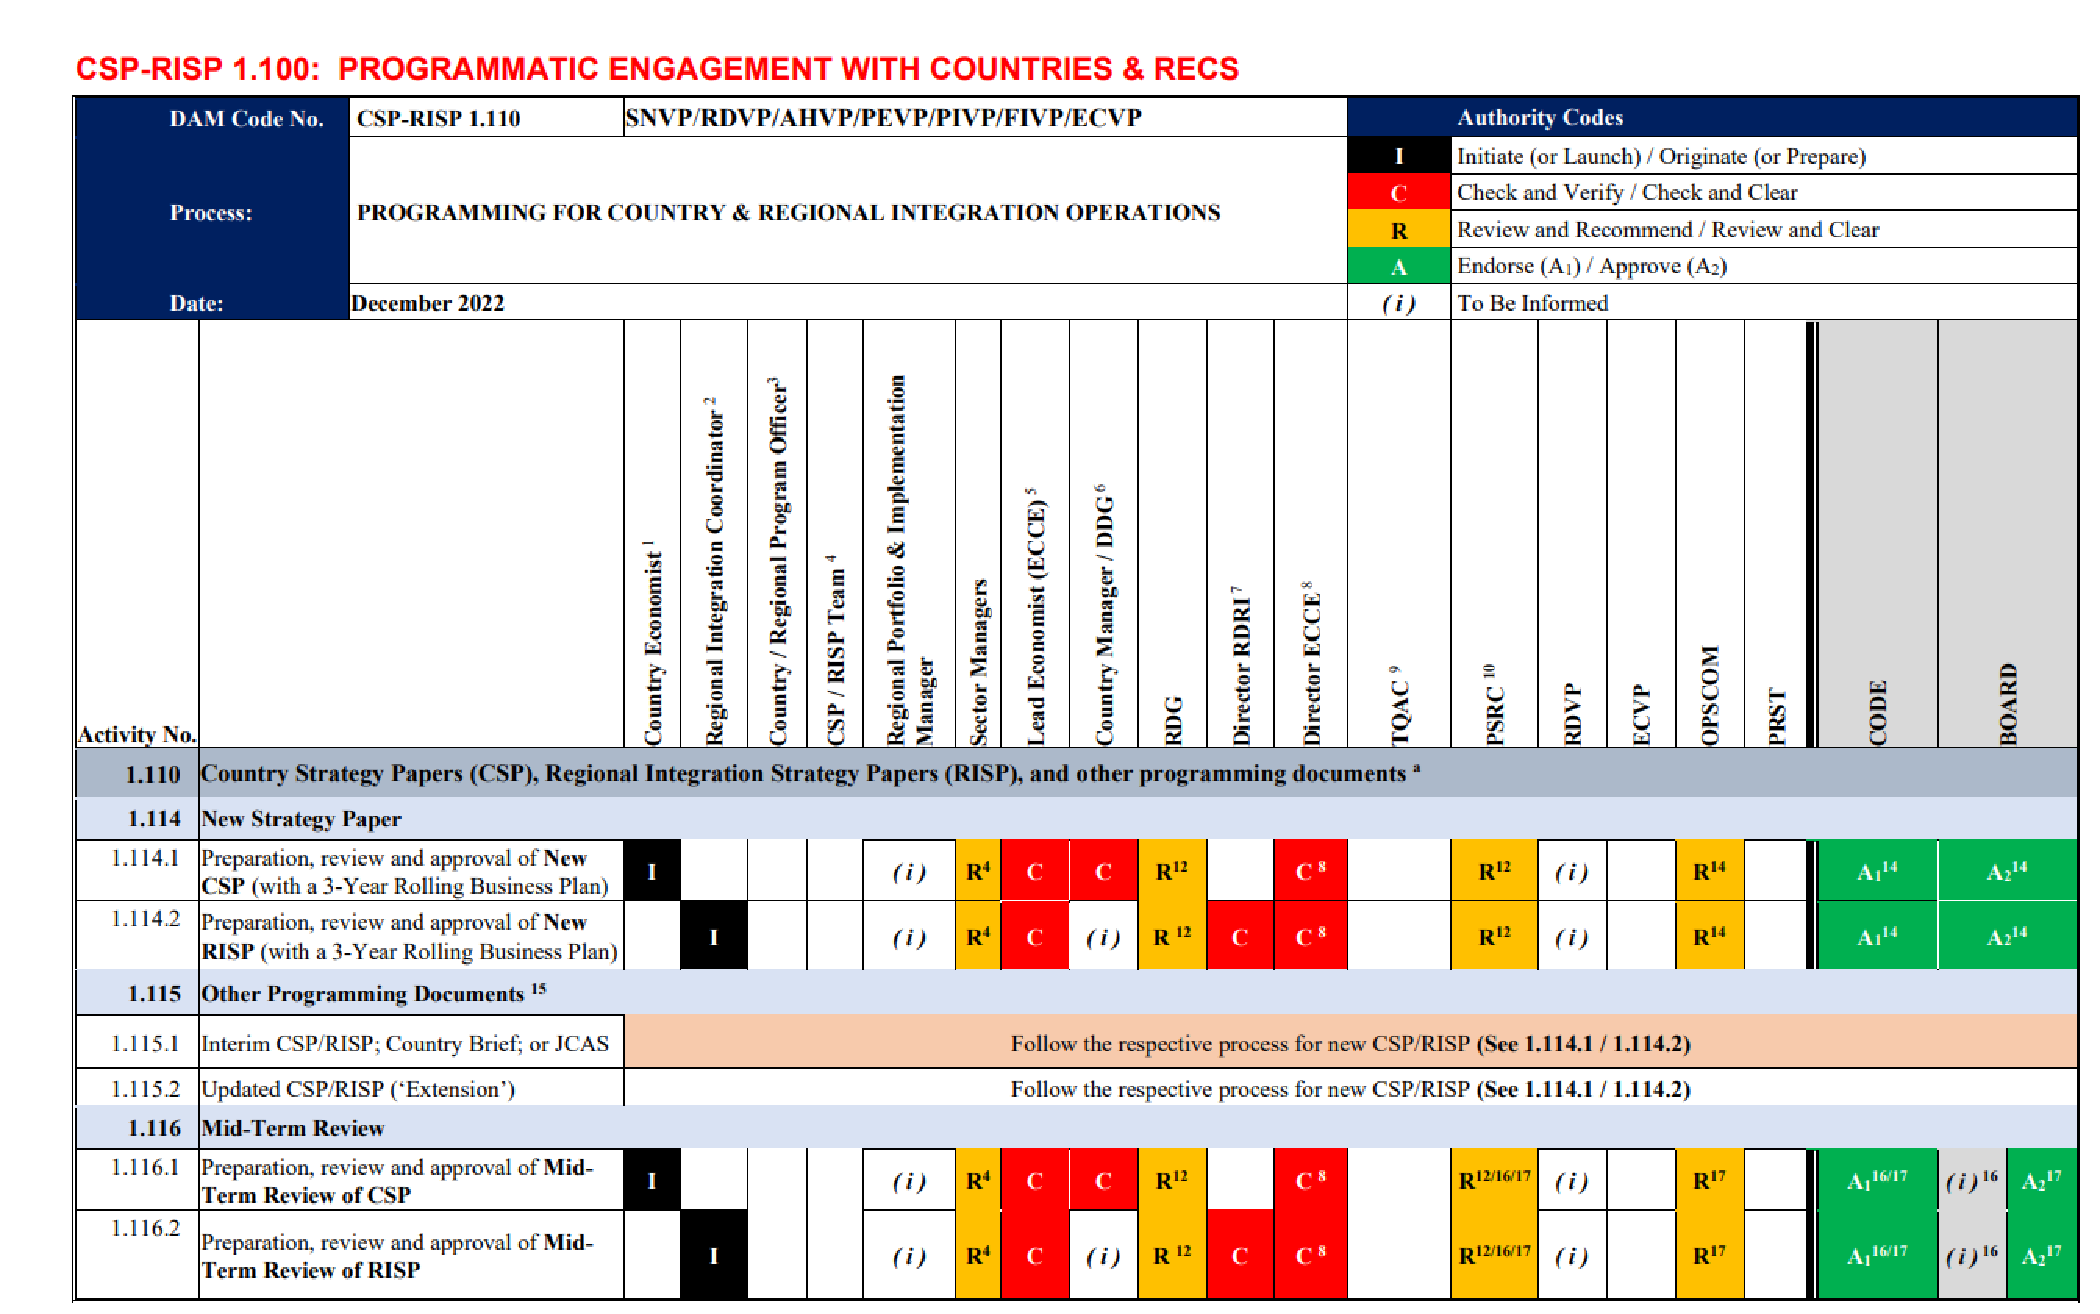
\includegraphics[width=0.88\linewidth]{figures/Capture d'écran 2026-09-16 184640.pdf}
    \caption{Example of a DAM page, showing the two stacked tables and the footnote band at the foot of the page.}
    \label{fig:DamPage}
\end{figure}

There are five authority codes but seventeen distinct notations, because most codes take a level, and the letter alone is therefore not the answer. Take C: on its own it denotes Check and Verify, and C1 and C2 are its two levels:

\begin{itemize}
\item \textbf{C1} --- examine the activity against a checklist of standards and preconditions, and allow it to proceed only if all of them are satisfied.
\item \textbf{C2} --- clear the activity as compliant with policy and regulation, after consulting the relevant departments.
\end{itemize}

Both are blocking obligations: the holder of a C1 or C2 code can halt the activity.

C3 and C4, however, are not levels of checking at all. They denote Consult, an unrelated obligation that happens to share the letter:

\begin{itemize}
\item \textbf{C3} --- obtain the opinion of an independent function (IDEV, BCRM) or of a knowledgeable expert.
\item \textbf{C4} --- the Board of Directors or the Board of Governors must be consulted, while the President or Management still holds the approval.
\end{itemize}

These are advisory obligations: the holder of a C3 or C4 code contributes an opinion but cannot halt the activity on that basis alone. The full notation, reproduced in Figure~\ref{fig:authoritycodes}, makes the extent of the ambiguity visible: a reader who resolves the letter without resolving its level can invert a blocking obligation into an advisory one, which is the single most consequential misreading the document permits.

\begin{figure}[htbp]
    \centering
    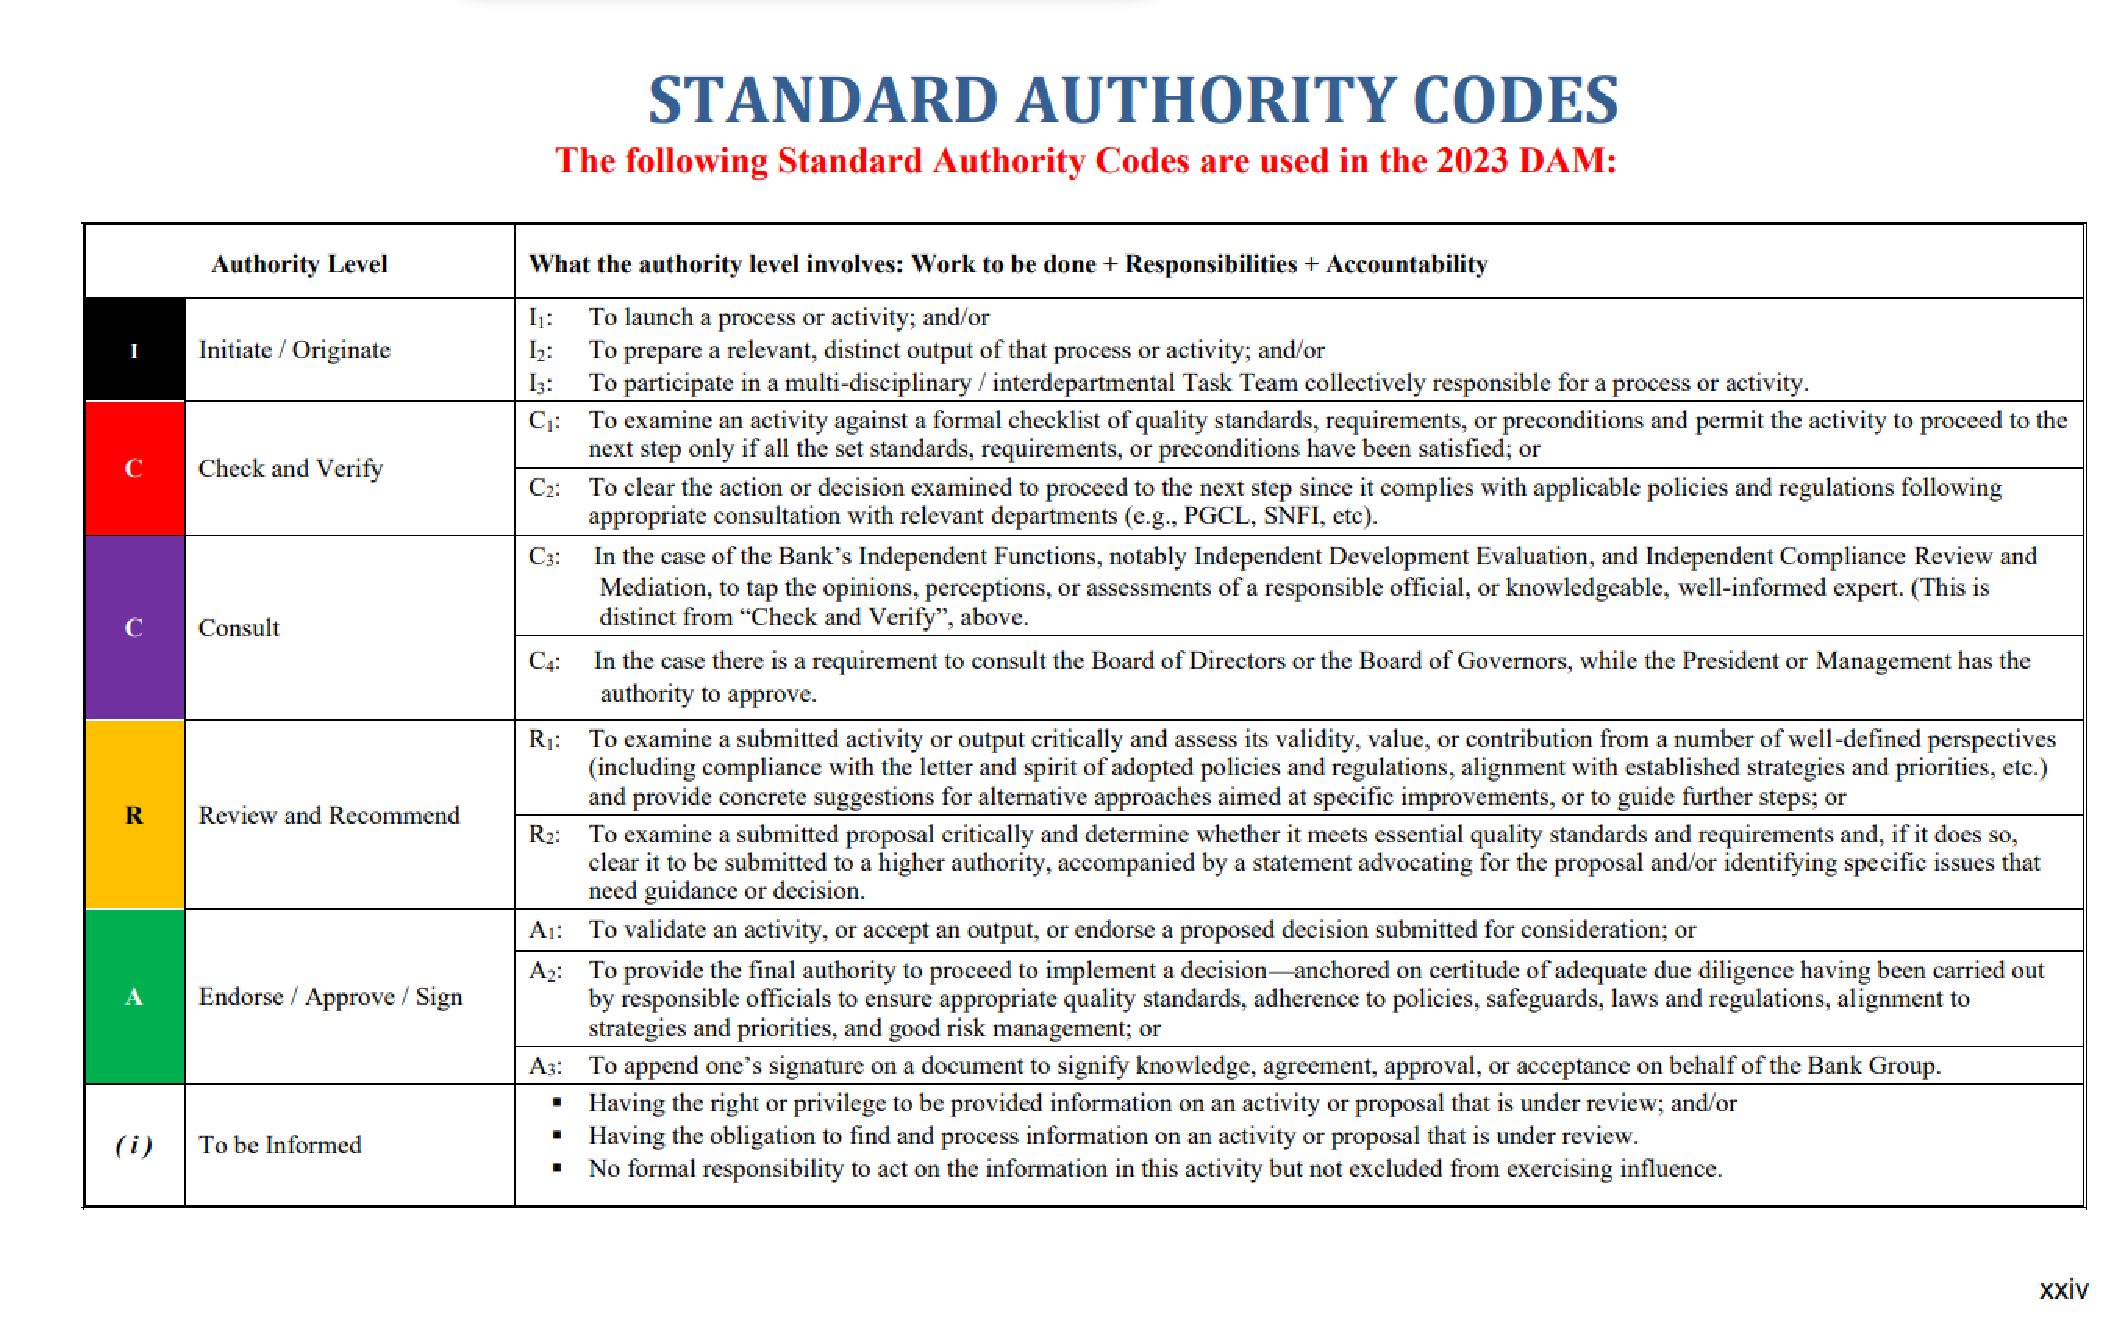
\includegraphics[width=0.88\linewidth]{figures/authority-codes.pdf}
    \caption{Authority-code legend, in which five codes expand into seventeen level-qualified notations.}
    \label{fig:authoritycodes}
\end{figure}

\subsubsection{Governance and Compliance Requirements}

The DAM is not a manual of procedures. It tells who can do something, but not how to do it. Clearly erroneous approvals would be likely to be picked up in normal organization reviews, as the individual consulted would know that it was beyond their authority. However, the DAM structure creates situations where an erroneous approval appears to be fully justified: two almost identical activities may have totally different approvers, and the person who is requested to approve is still a valid approver for this activity category as a whole — they have no way of knowing, from their position, that this particular case is assigned to someone else. This section covers the requirements that the document places on persons who wish to.This section addresses conditions for the proper interpretation of the document without any consideration of hierarchy.\\[0.3cm]
Approximation is allowed to a certain degree in most reference materials. The worst thing that can happen if an employee gets the meeting time wrong is that they miss the meeting and are able to catch up with the minutes later. This is how the DAM does not work. When a staff member misunderstands it, or misses an important role, in the course of carrying out a task, that task moves forward without the required authorisation. There is no immediate rejection or alert. The outcome is not that the reader is left without an answer, but that the reader proceeds from a self-assured but partial answer, with no hint of the opposite.\\[0.3cm]
A response can be perfectly accurate and still be misunderstood. The different tables in the DAM answer questions like “who approves X”, but by only naming the approver it conceals the need to consult others, as approval and verification are often interdependent stages of the same task – something FR4 aims to avoid. This is not an uncommon situation. Of the 216 activities that have an identified approver, 81 have no documented check or validation step. The mismatch was discovered during a trial meeting with the client – while demonstrating the agent by asking who authorises X, Yasser noticed that the response also had no check/verify function. His reasoning was that an experienced employee can easily see the connection between an approver and the person who verifies it, but a new employee may not automatically see this relationship and could easily miss it. That query showed the discrepancy, and hence the system is now giving a documented check/verification step irrespective of the initial query asked.\\[0.3cm]
Finally, the DAM file can be hard to understand for new staff without proper guidance. The staff member may miss crucial information while reading the document.
\subsubsection{Challenges in Consulting the DAM in Practice}

One of the few weaknesses of Consulting the DAM in Practice is that it takes time just to find the file in the local environment among all the other documents, and once it's found, the user still needs to scroll all the way down to the specific task that he/she needs. in some cases, even after finising it, the user can find some difficulties understanding the instruction provided by the DAM tables clearly. This causes staff to call someone more experienced to explain it.

Table~\ref{tab:twintasks} shows the problem in its sharpest form: two activities whose titles differ only in a monetary band, sitting on consecutive pages, carrying different approvers. A reader who matches on the wording alone and does not check the threshold will name the wrong approver while believing the match was exact.

\begin{table}[h]
\centering
\caption{Two near-identical activities with different approvers.}
\label{tab:twintasks}
\begin{tabular}{|l|c|p{0.4\textwidth}|l|}
\hline
\rowcolor{myblue}
\textcolor{white}{\textbf{ID}} & \textcolor{white}{\textbf{Page}} & \textcolor{white}{\textbf{Title}} & \textcolor{white}{\textbf{Approver}} \\
\hline
2.432.4.a & 43 & Individual Consultant: $\leq$ UA 50,000 & Sector Manager \\
\hline
2.433.4.c & 44 & Individual Consultant: $>$ UA 250,000 & PRC \\
\hline
\end{tabular}
\end{table}


\subsection{Study of Existing Systems}
\label{sec:existingsystems}

With the DAM's demands on readers now clear, the natural question is whether an existing tool already meets them.  We can examine two categories of tools against these weaknesses to see whether any address what the DAM lacks. The first method involves consulting the DAM and performing a manual search. The second, however, is a tool that requires using a generic question-answering assistant designed to analyze the submitted file and answer the user's question. The study of both of these systems makes it possible to better understand the needs and expectations regarding the outcome required from the DAM AI Agent.

\subsubsection{Manual Consultation and Document Search}

The current process is manual consultation of the PDF, supported by the basic search the PDF Viewer tool provides (Acrobat, Foxit,...). The Keyword search finds a character string, which helps when the staff already knows the exact title of an activity or its identifier, and helps very little otherwise. Searching for the word "approve" will return either the explanatory authority code table on the first few pages or every table in the DAM. Searching for a partially remembered activity name returns nothing at all unless the remembered words match the printed ones exactly.\\[0.3cm]

More importantly, text search returns locations not answers. It can tell the staff that a term exist in page X. It cannot tell them who approves the activity described there since that requires understanding that the pages holds a table and that the tables in the DAM have a complexe visual design and that the same action can change depending on the authority level and the footnote attached to it.

\subsubsection{Generic Document Question-Answering Assistants}

A second category of existing solustion is the General purpose document assistant tools such as ChatPDF \citep{chatpdf}, NotebookLM \citep{notebooklm} or Microsoft Copilot's file upload mode \citep{ms365copilot}. These tools typically function by splitting the document into passages, embed those passages into vectors, retrieve the passage similar to the question and then pass them to a language model that writes an answer. This is standard retrieval-augmented generation, or RAG \citep{lewis2020rag}.\\[0.3cm]
This approach performs well on the conventional text heavy documents but breaks on this document for a reason that the DAM is structural rather than literary. When a page of the DAM is converted to plain text, the spatial relationship that carry its meaning are destroyed. The rotated header that identified a column becomes a stray string lost in the extracted corpus, disconnected from the footnotes beneath it. A retrieved passage may therefore contain the activity name and the authority code letter without preserving the information that the authority code belonged to a specific cell and has a specific footnote or authority level. in that case the model is left working from a text that has already lost the answer, and produces a confident answer either ways.

\begin{figure}[htbp]
\centering
\begin{subfigure}[b]{\linewidth}
\centering
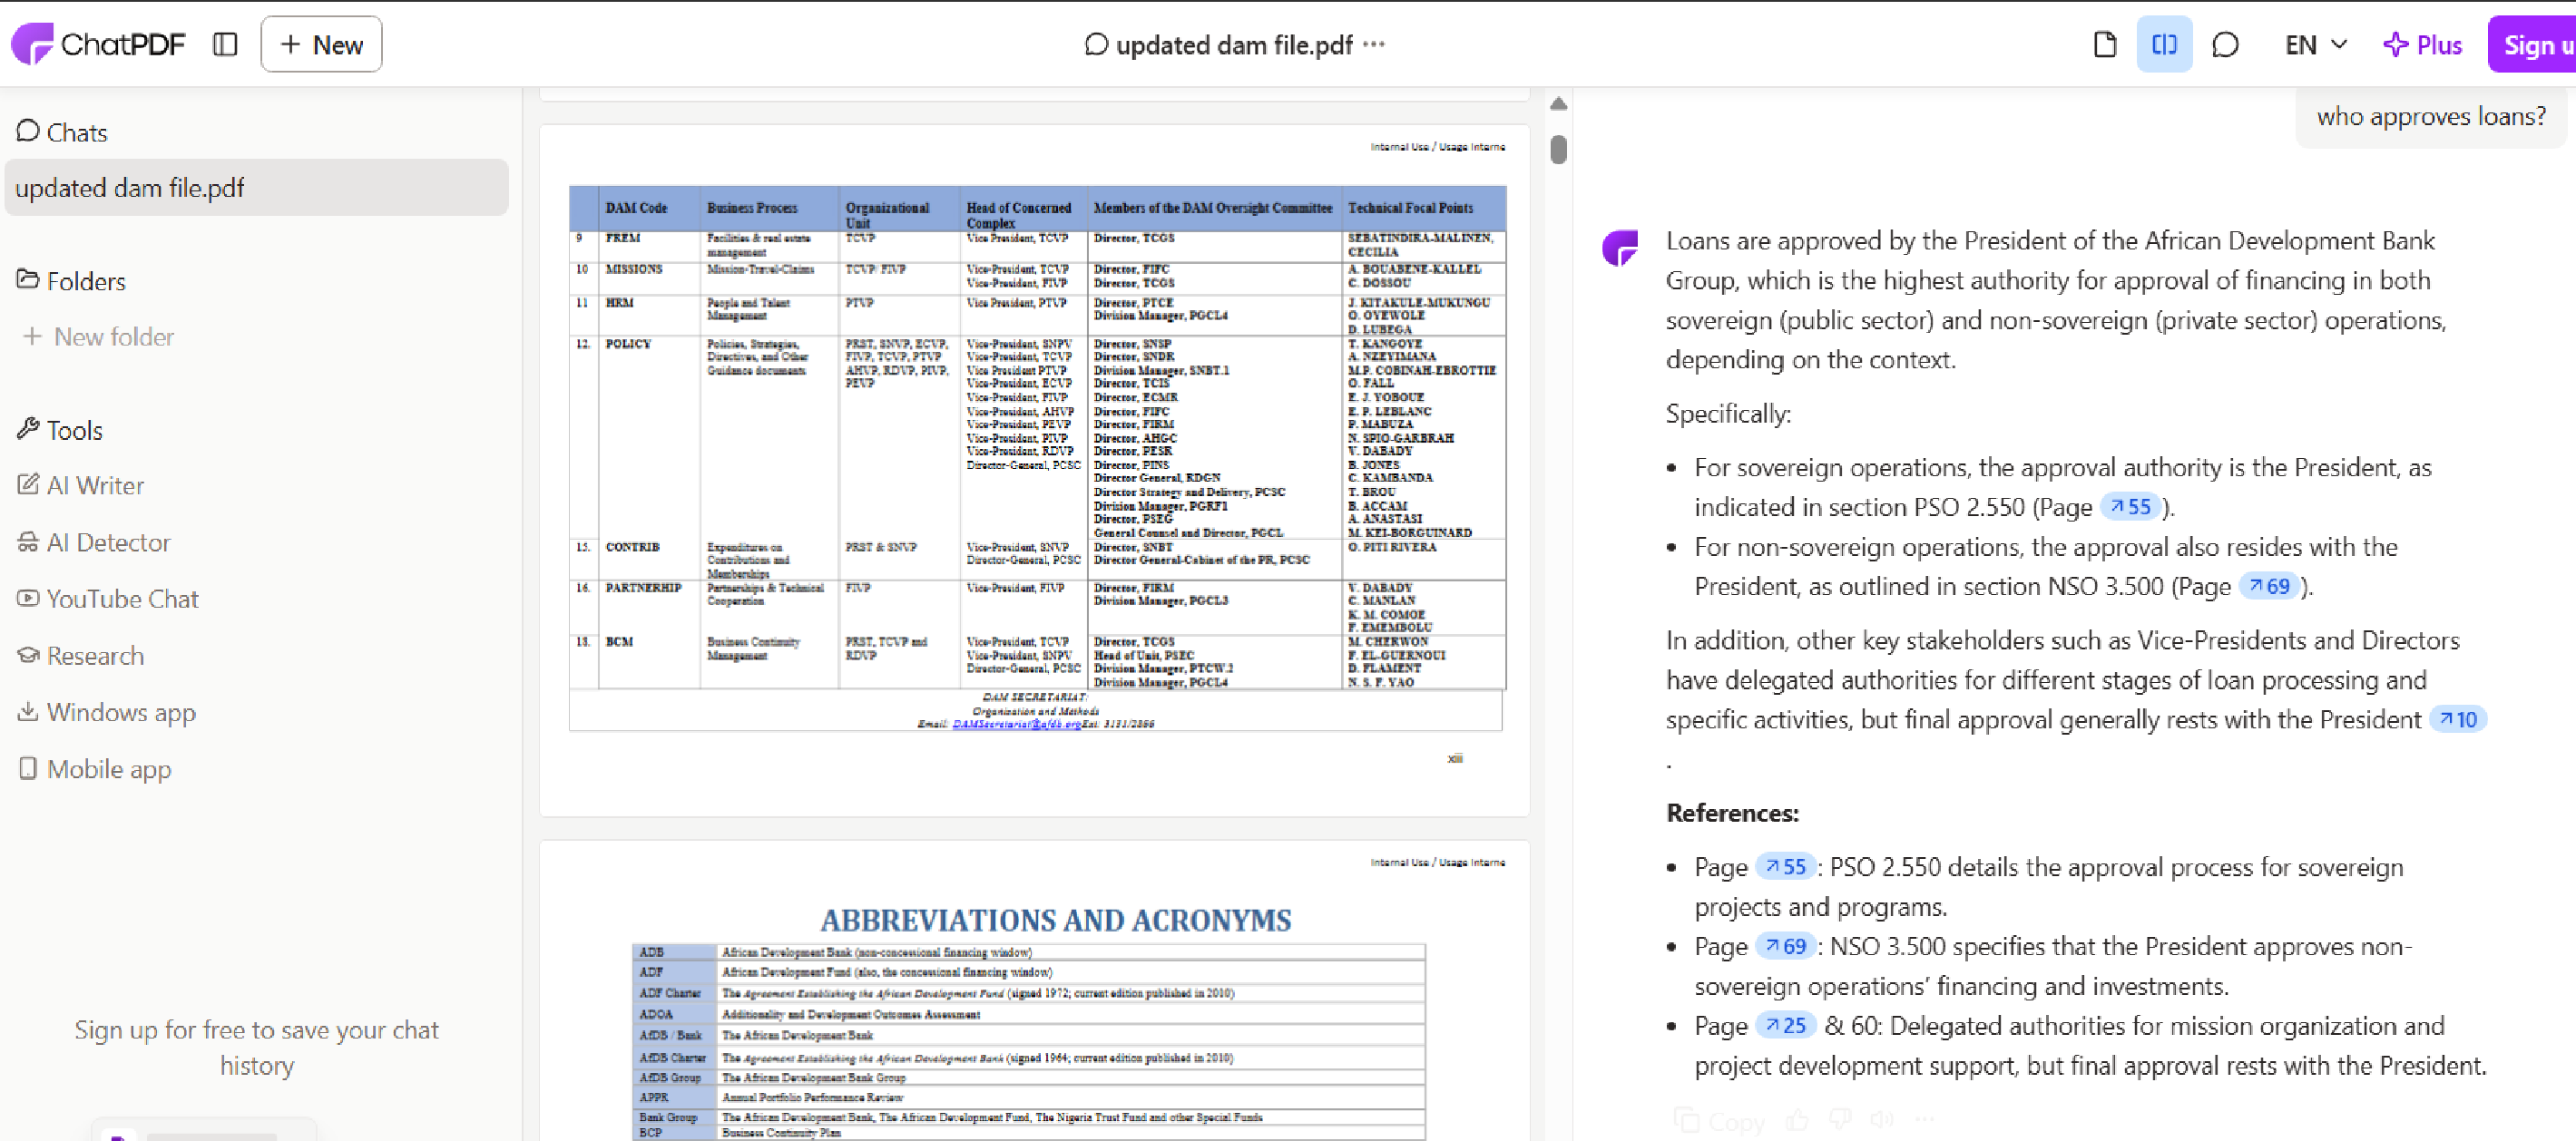
\includegraphics[width=0.92\linewidth]{figures/chatpdf-loans.pdf}
\caption{``Who approves loans?''}
\label{fig:chatpdf-loans}
\end{subfigure}
\par\bigskip
\begin{subfigure}[b]{\linewidth}
\centering
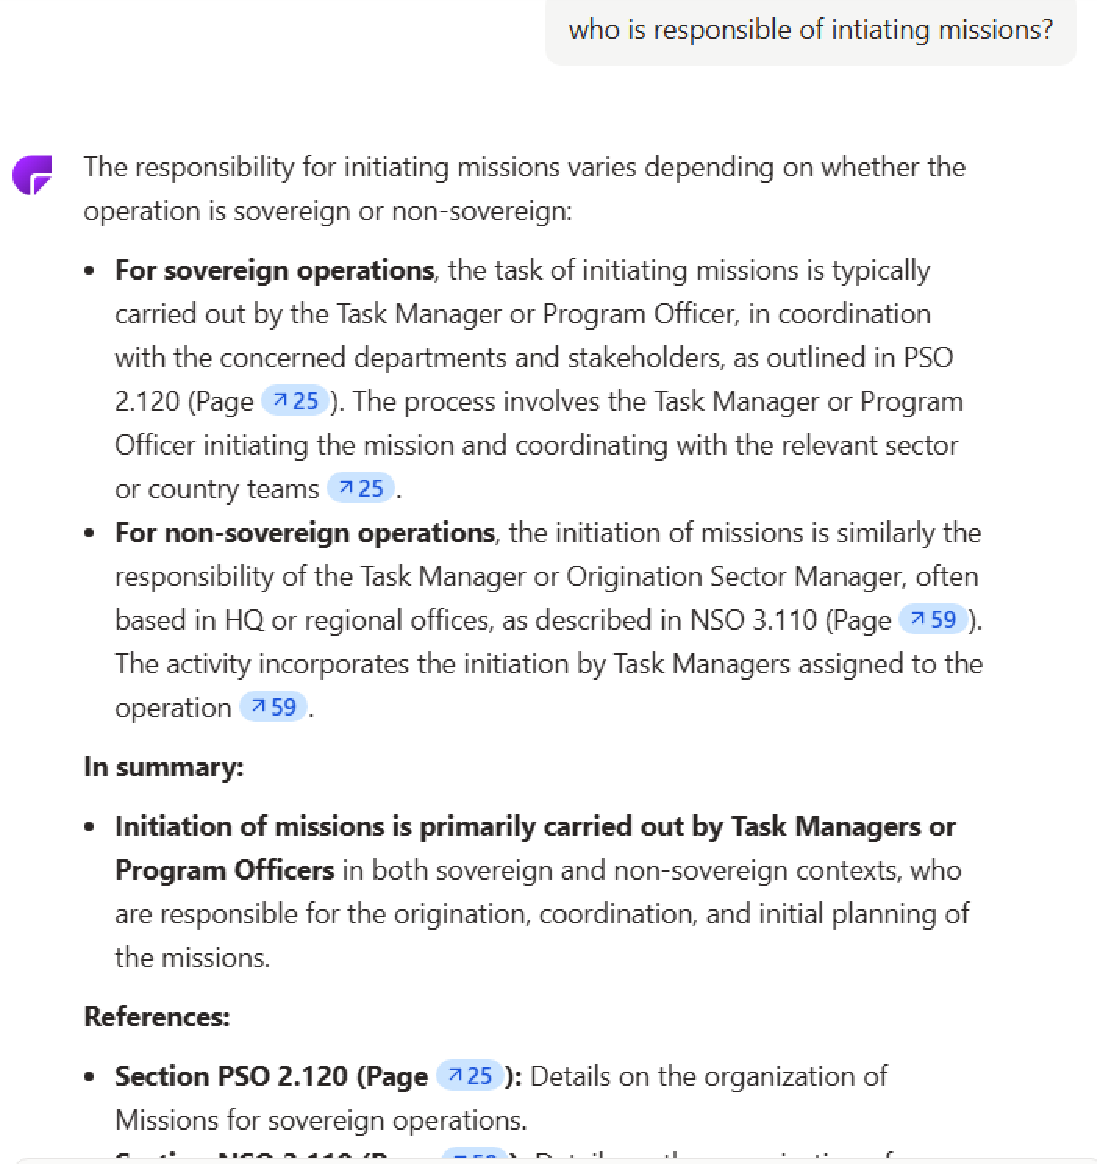
\includegraphics[width=0.92\linewidth]{figures/chatpdf-missions.pdf}
\caption{``Who is responsible for initiating missions?''}
\label{fig:chatpdf-missions}
\end{subfigure}
\caption{ChatPDF's answers to two DAM authority questions, with page citations it generated automatically. The two exchanges are stacked rather than placed side by side so that the wording of each answer stays legible at normal page width.}
\label{fig:chatpdf}
\end{figure}

To test this directly, two pages of the DAM were uploaded to ChatPDF and asked "who approves loans?" and "who is responsible for initiating missions?" (Figure~\ref{fig:chatpdf}). Both answers were fluent, well-structured, and included automatically generated page citations. Checked against this project's own extracted data, however, neither holds up at the level of detail the DAM actually records. The DAM lists the President as an approver in exactly one context — a staff-seniority escalation ladder for mission-related sign-off — not as a general final approver for loans. The specific page ChatPDF cited for loan approval in fact records a different and more complex set of roles, one of which could not even be confidently resolved to a name during this project's own extraction. The mission-initiation answer merges several distinct activities sharing a common process code into a single summary, silently dropping at least one case with a different initiator entirely. Both answers illustrate the mechanism described above: the tool produces something fluent and well-organised from a page whose spatial structure it has already discarded, and the fluency of the result gives no indication of where it has quietly generalised past what the actual row records.

\subsubsection{Critical Analysis: Limitations of Current Approaches}

Both approaches ultimately encounter a fundamental challenge: they lack an awareness of error. This is the failure mode surveyed across generative systems as hallucination\citep{ji2023hallucination}, and it is particularly consequential here, because a confidently phrased wrong approver is indistinguishable to the reader from a correct one. When a search engine produces results or a language model generates text, neither system differentiates between a supported answer and one that lacks justification. This distinction is crucial for compliance purposes.

Table~\ref{tab:existing} assesses both categories against the needs established earlier in this section, alongside the approach taken in this work.

\begin{table}[h]
\centering
\caption{Existing approaches assessed against the needs of this project.}
\label{tab:existing}
\small
\begin{tabular}{|p{0.3\textwidth}|c|c|c|c|}
\hline
\rowcolor{myblue}
\textcolor{white}{\textbf{Requirement}} &
\textcolor{white}{\textbf{Search}} &
\textcolor{white}{\textbf{Assistants}} &
\textcolor{white}{\textbf{This work}} \\
\hline
Preserves positional table meaning & No & No & Yes \\ \hline
Answers a question, not a location & No & Yes & Yes \\ \hline
Answer traceable to a source row & No & No & Yes \\ \hline
Refuses when it cannot answer & N/A & No & Yes \\ \hline
Surfaces mandatory obligations & No & No & Yes \\ \hline
Tolerates typos and loose phrasing & No & Yes & Yes \\ \hline
Document stays inside the institution & Yes & No & Yes \\ \hline
No per-page or licence cost & Yes & Partly & Yes \\ \hline
Deployable within this project & Yes & Yes & Yes \\ \hline
\end{tabular}
\end{table}

The table above presents a comparative analysis of the two existing systems for reading the DAM document. Three major differences between the systems are evident.
First, the question-answering assistant can tolerate typos within the document, whereas the manual search method does not account for such errors.
Second, the question-answering assistant differs from the manual search method by its ability to answer user questions regarding the DAM document, a capability not available with the manual search method.
Third and finally, the manual search method differs from the question-answering assistant in terms of security. Submitting an internal, confidential document of this magnitude to a generic question-answering assistant, one not created or licensed by the AFDB, constitutes a security breach. Consequently, a manual search within the document can be viewed as a less efficient but more secure solution, as it relies on no external tools that could compromise the security and confidentiality of the DAM document.\\[0.2cm]
Thus, a conclusion can be drawn from this comparative analysis of the two previously used methods. The DAM AI Agent must, first, be capable of functioning even in the presence of typos. Next, it must accurately and precisely answer the various questions a user might ask. Finally, the DAM AI Agent must comply with AFDB security standards, and the document submitted to it must remain confidential. This last point will be explained further in the Authentication section of Chapter 5.

\section{Functional Needs Analysis}

The gaps identified above translate directly into requirements: each one traces back to a
specific limitation of manual search or generic assistants documented in the preceding
section.

\subsection{Functional requirements}

The functional requirements are categorised into two groups. Requirements FR1 to FR10 pertain to the fundamental question-answering capability and derive from current document consultation practices. Requirements FR11 to FR15 address the platform capabilities introduced in the project's second phase, which transform the system from a lookup tool into an application usable inside an institution. Table~\ref{tab:fr} describes each of them.

Every requirement listed satisfies two conditions. It corresponds to a need observed in the way the document is consulted, rather than to a capability that merely seemed attractive to build; and it is met by the delivered system. Requirements that failed either condition were removed rather than retained as statements of intent, since a requirements table describing intentions cannot be used to evaluate what was actually produced.

\begin{longtable}{|p{0.08\textwidth}|p{0.26\textwidth}|p{0.54\textwidth}|}
\caption{Functional requirements.}\label{tab:fr}\\
\hline
\rowcolor{myblue}\textcolor{white}{\textbf{Ref.}} & \textcolor{white}{\textbf{Requirement}} & \textcolor{white}{\textbf{Description}} \\
\hline
\endfirsthead
\hline
\rowcolor{myblue}\textcolor{white}{\textbf{Ref.}} & \textcolor{white}{\textbf{Requirement}} & \textcolor{white}{\textbf{Description}} \\
\hline
\endhead
FR1 & Direct identifier lookup & Given a valid activity identifier, the system returns that activity's recorded authority information with full confidence and no ambiguity. \\ \hline
FR2 & Natural-language lookup & Given a question describing an activity by name rather than by identifier, the system resolves it to the correct activity and reports how confident that resolution is. \\ \hline
FR3 & Authority-role queries & For a resolved activity, the system answers who approves, reviews, checks, initiates, or must be informed, using the document's own notation. \\ \hline
FR4 & Mandatory obligation surfacing & Whatever the question asked, the system always surfaces a recorded check-and-verify obligation and, where present, the informed parties. \\ \hline
FR5 & Cross-reference resolution & Where an activity's row is a pointer to another activity, the system follows the pointer automatically rather than reporting that no responsibilities exist. \\ \hline
FR6 & Typing and phrasing tolerance & The system tolerates common misspellings and phrasing variation without requiring the document's exact vocabulary. \\ \hline
FR7 & Honest refusal & For an identifier that does not exist, or a question outside the document's subject matter, the system says so explicitly instead of returning a best guess. \\ \hline
FR8 & Conversational continuity & A follow-up question that does not restate its subject is answered against the activity discussed immediately before. \\ \hline
FR9 & Structural analytics & The system exposes an overview of the document's own structure: node counts, authority-code distribution, roles most frequently involved, and per-chapter breakdowns. \\ \hline
FR10 & Multilingual questions & Questions asked in French, Spanish, Portuguese, or Arabic are answered in the language they were asked in, without translating role names or identifiers. \\ \hline
FR11 & Authenticated access & Access to the application requires authentication, and analytical features are restricted to authorised roles. \\ \hline
FR12 & Voice input & A user can dictate a question instead of typing it, in any of the supported interface languages. \\ \hline
FR13 & Document attachment & A user can attach a supporting document to a conversation and ask questions about its content, with answers from that source clearly distinguished from answers grounded in the DAM. \\ \hline
FR14 & Localised conversation interface & The conversation interface, including its controls and its answer provenance labels, is available in each supported language, with right-to-left layout applied for Arabic. \\ \hline
FR15 & Conversation sharing & A user can grant a colleague read-only access to a conversation, either by naming them directly or through an expiring link encoded as a QR code, with shared views reflecting new messages without requiring a page reload. \\ \hline
\end{longtable}

\subsection{Non-Functional Requirements}

Where the functional requirements state what the system must do, the non-functional requirements state the qualities it must exhibit while doing it. They are not secondary. NFR1 in particular, which forbids any answer from naming a role or code the source document does not record for that activity, takes precedence over fluency, latency, and every other consideration in the table: a system of this kind that is pleasant to use and occasionally wrong is worse than no system at all, because it transfers confidence without transferring correctness. The remaining requirements span traceability, availability, reproducibility, portability, and the handling of credentials and uploaded files. Table~\ref{tab:nfr} details each one.

\begin{longtable}{|p{0.08\textwidth}|p{0.26\textwidth}|p{0.54\textwidth}|}
\caption{Non-functional requirements.}\label{tab:nfr}\\
\hline
\rowcolor{myblue}\textcolor{white}{\textbf{Ref.}} & \textcolor{white}{\textbf{Requirement}} & \textcolor{white}{\textbf{Description}} \\
\hline
\endfirsthead
\hline
\rowcolor{myblue}\textcolor{white}{\textbf{Ref.}} & \textcolor{white}{\textbf{Requirement}} & \textcolor{white}{\textbf{Description}} \\
\hline
\endhead
NFR1 & Factual fidelity & No answer may contain a role, code, or qualification that is not recorded in the source document for that activity. This requirement takes precedence over fluency, speed, and every other consideration. \\ \hline
NFR2 & Traceability & Every answer must be attributable to a specific activity record so that a user can verify it against the printed document. \\ \hline
NFR3 & Availability without external services & Core lookup must work when no language model provider is reachable, degrading to template answers rather than failing. \\ \hline
NFR4 & Response time & Answers should return within a few seconds on the free hosting tier used for deployment, which rules out re-parsing the document per request. \\ \hline
NFR5 & Reproducibility & The same question must produce the same underlying facts on every run, independent of any model's sampling behaviour. \\ \hline
NFR6 & Portability & The system must run identically on a developer machine and on the hosting platform, without environment-specific configuration. \\ \hline
NFR7 & Usability on any device & The interface must remain usable on a phone, since consultation often happens away from a desk. \\ \hline
NFR8 & Credential protection & Authentication credentials must never be stored in recoverable form, and session tokens must expire. \\ \hline
NFR9 & Upload safety & Attached documents must be constrained by type and size, and must never be executed or interpreted as anything other than text to be read. \\ \hline
\end{longtable}

\subsection{Project Constraints}

The conditions below were fixed before any design decision was taken, and each one closed off an approach that would otherwise have been reasonable. They are recorded here because several choices defended later in this report, particularly the preference for lexical retrieval over learned embeddings and the decision to cache the parsed knowledge base at build time, follow directly from them rather than from a free comparison of alternatives. Table~\ref{tab:constraints} sets out each constraint and what it ruled out.

\begin{longtable}{|p{0.30\textwidth}|p{0.58\textwidth}|}
\caption{Project constraints.}\label{tab:constraints}\\
\hline
\rowcolor{myblue}\textcolor{white}{\textbf{Constraint}} & \textcolor{white}{\textbf{Consequence for the project}} \\
\hline
\endfirsthead
\hline
\rowcolor{myblue}\textcolor{white}{\textbf{Constraint}} & \textcolor{white}{\textbf{Consequence for the project}} \\
\hline
\endhead
No labelled training data & No query-and-answer pairs and no annotated tables existed, which ruled out training a supervised model and pushed retrieval toward lexical methods that need no training corpus. \\ \hline
Document scope & The full DAM exceeds 250 pages. Work was scoped to a 79-page subset covering three chapters, with the remainder left as future work. \\ \hline
No infrastructure budget & Deployment had to fit within free hosting tiers, which constrained memory use and forced the parsed knowledge base to be cached at build time rather than rebuilt on startup. \\ \hline
Verification against the source & Because no ground-truth dataset existed, correctness had to be established by comparison against real pages of the document, which set the pace of the data understanding phase. \\ \hline
\end{longtable}

\section{Proposed Solution}

The requirements above rule out both alternatives surveyed earlier: manual search cannot
answer a question, and a generic assistant cannot be trusted to answer it correctly. The
system described in the rest of this chapter is built to do both, starting from a general
design principle and then the four-layer architecture that implements it.

\subsection{General Presentation of the Solution}

The proposed system delineates two distinct tasks that conventional assistants typically merge: ascertaining factual content and determining the appropriate manner of expression. The factual information is extracted from a structured knowledge base, created by analyzing the document once offline, utilizing rules derived from the document’s own structure and subsequently validated against printed materials. In contrast, phrasing is managed by a language model, which rewords facts that have been previously retrieved.

In between these two layers, a crucial verification process occurs. Before any generated response is presented to the user, it undergoes a comparison with the retrieved facts. Any response that omits or modifies a role name is discarded in favor of a predetermined template. Consequently, users receive accurate answers, albeit delivered in a less conversational format. This verification mechanism ensures the language model's safe application within this context. It is described in detail in Chapter~4.

\subsection{Global System Architecture}

The system comprises four distinct layers. The offline extraction layer converts the source PDF into a validated set of nodes, which are subsequently cached and included with the application. The knowledge layer utilizes this node set as a directed graph, enabling efficient searches and lookups. The agent layer interprets user inquiries, translates them into actionable tasks, formulates definitive responses, and utilizes the language model along with a verification process. Finally, the presentation layer interfaces with the agent through a REST framework, facilitating conversation, document attachment, export, sharing, and analytics features.

Figure~\ref{fig:architecture} shows how these four layers relate, and in particular where the boundary between offline and online work falls.

\begin{figure}[htbp]
\centering
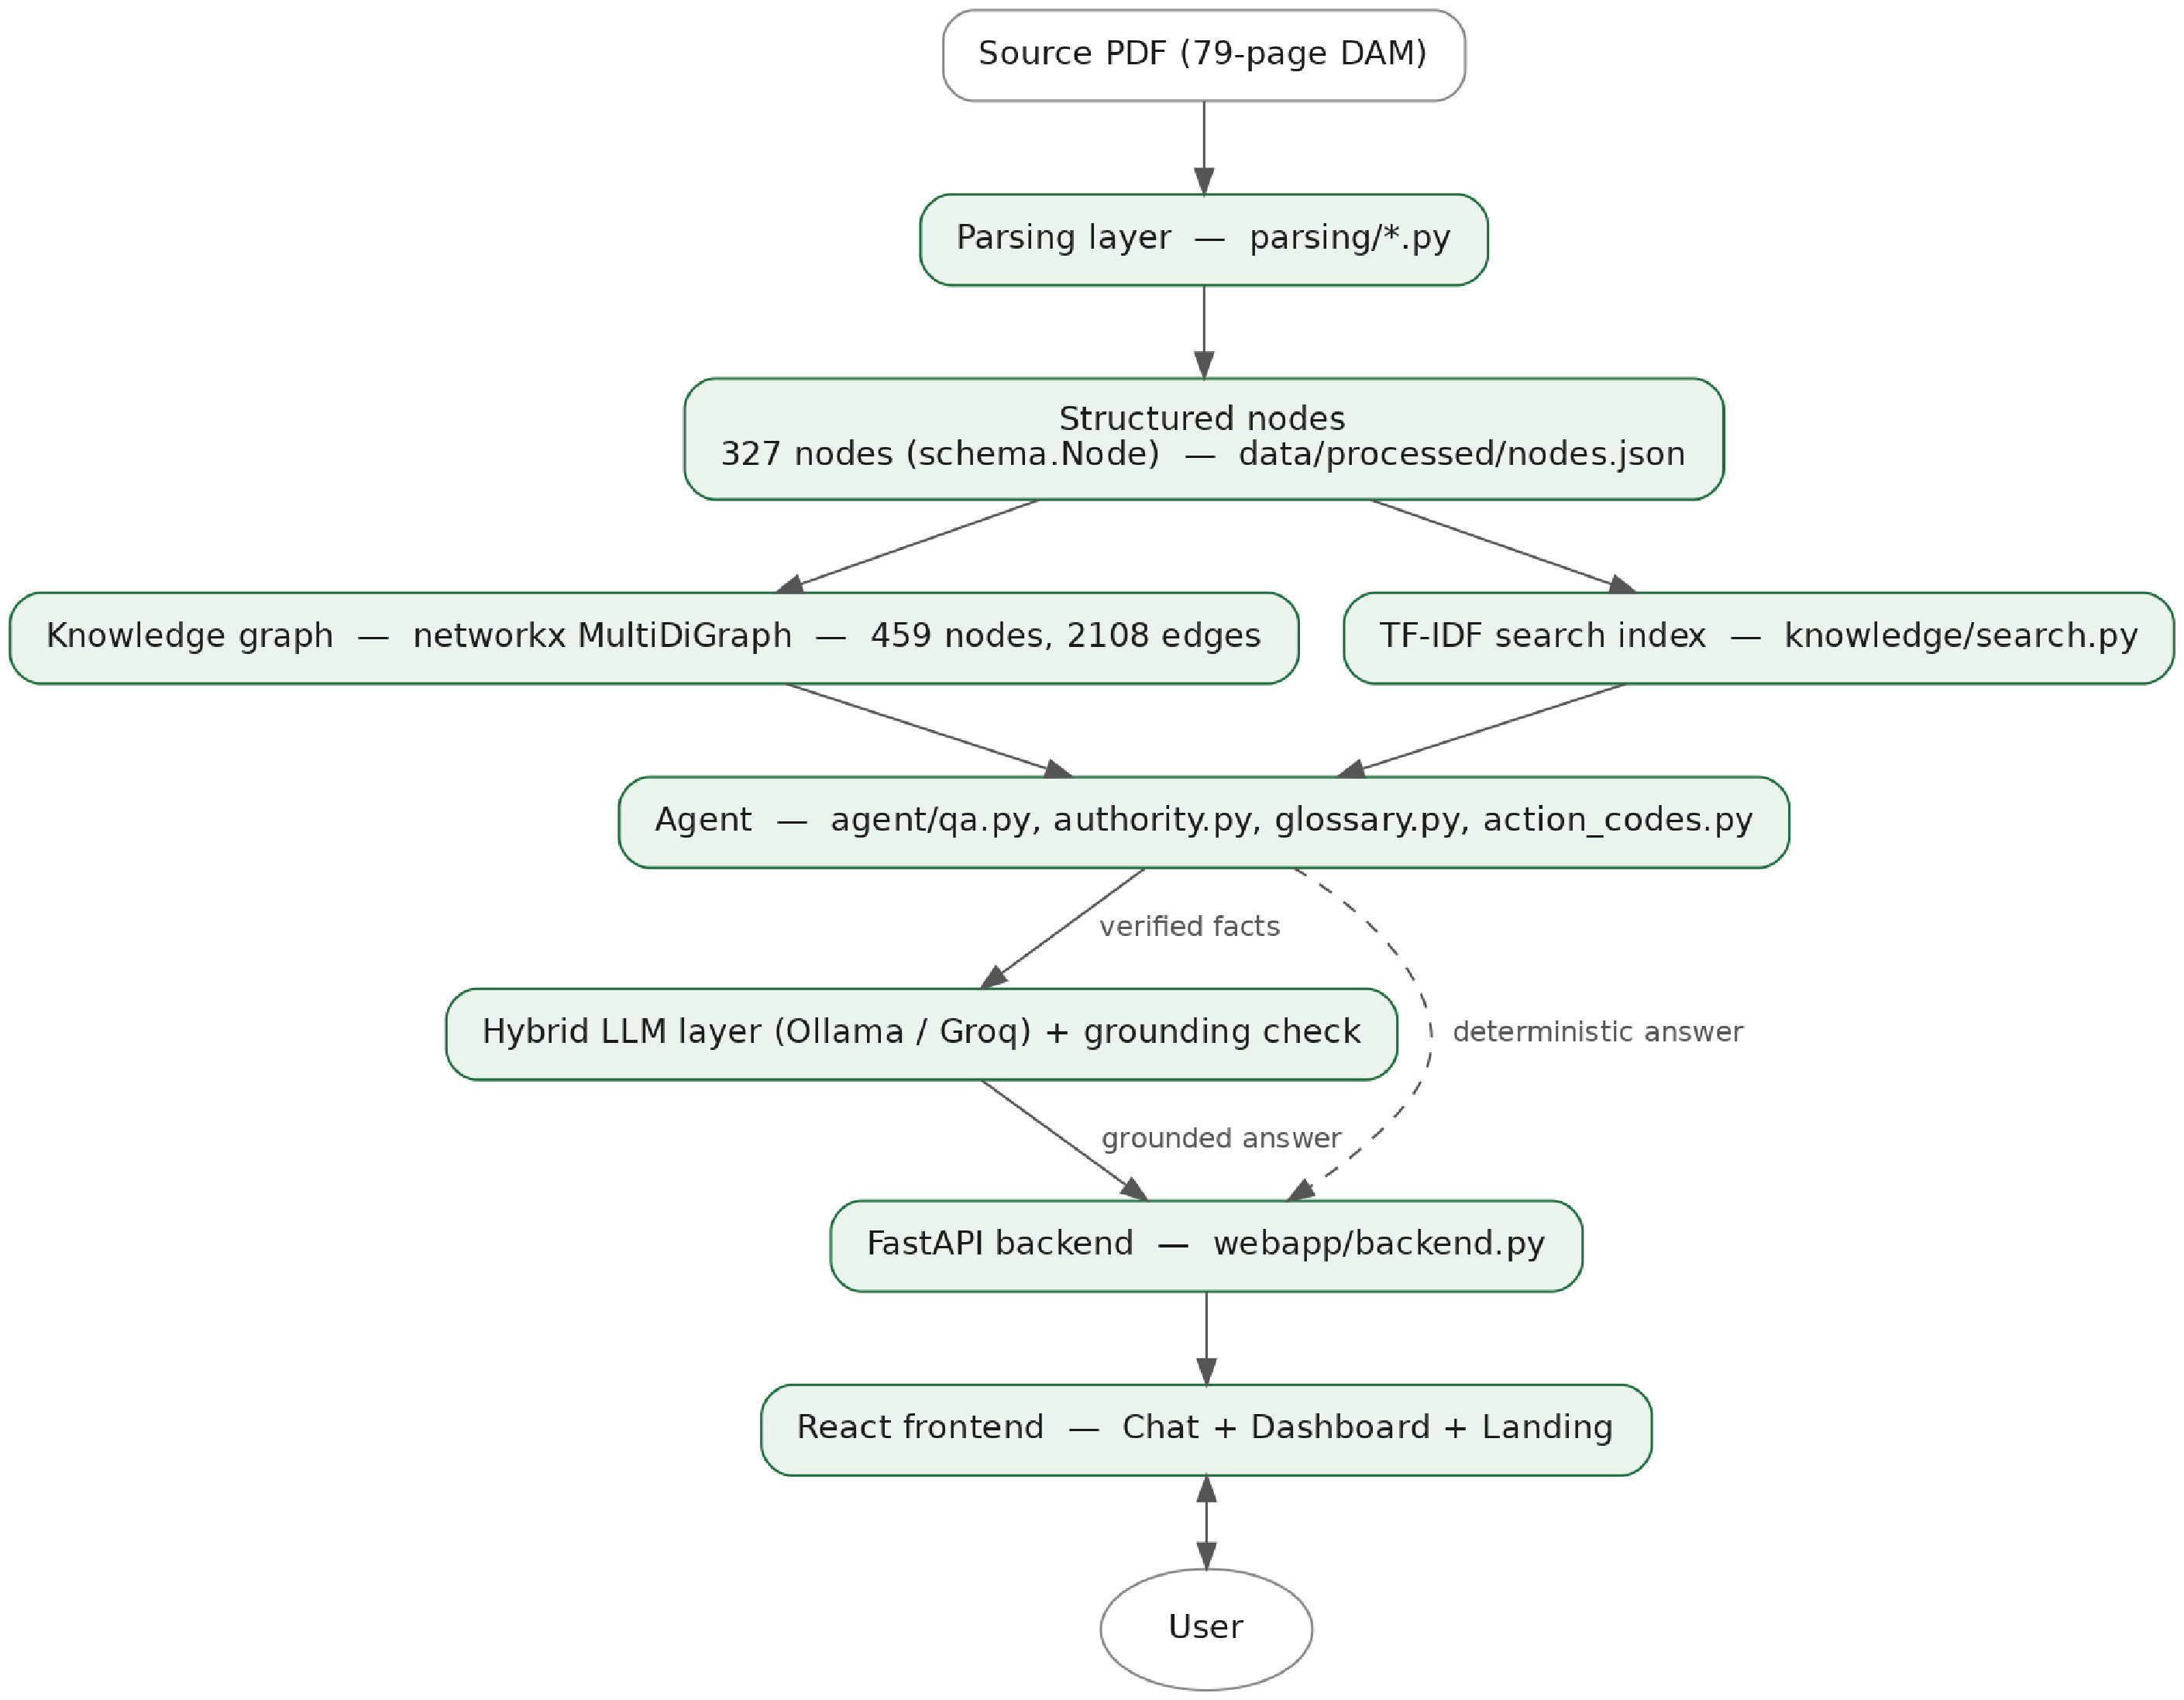
\includegraphics[width=0.94\textwidth,height=0.88\textheight,keepaspectratio]{figures/fig1_architecture.pdf}
\caption{Global architecture of the proposed system, from source document to user-facing answer.}
\label{fig:architecture}
\end{figure}

One notable consequence of this separation is that, because extraction occurs offline and its output is cached, the running application interacts exclusively with a prepared set of nodes stored in memory at startup, never directly accessing the PDF. This approach was adopted for deployment efficiency,

\subsection{Selected Technologies}

Several tools and technologies were selected to serve a specific purpose in the construction of the system, and each was chosen against the constraints recorded in Table~\ref{tab:constraints} rather than on general merit. Table~\ref{tab:tech} lists each technology and the role it plays.

\begin{longtable}{|p{0.26\textwidth}|p{0.62\textwidth}|}
\caption{Selected technologies and their role in the system.}\label{tab:tech}\\
\hline
\rowcolor{myblue}\textcolor{white}{\textbf{Technology}} & \textcolor{white}{\textbf{Role in the system}} \\
\hline
\endfirsthead
\hline
\rowcolor{myblue}\textcolor{white}{\textbf{Technology}} & \textcolor{white}{\textbf{Role in the system}} \\
\hline
\endhead
Python & Language for extraction, knowledge base, agent, and backend. \\ \hline
pdfplumber\citep{pdfplumber} & Character- and word-level PDF extraction with positional coordinates, which is what makes geometric reasoning about rotated headers and superscripts possible. \\ \hline
Pydantic\citep{pydantic_docs} & Schema definition and validation for the node model, so malformed records fail at construction rather than at query time. \\ \hline
networkx\citep{hagberg2008networkx} & Knowledge graph construction and traversal, using a directed multigraph so that a role can hold several distinct responsibilities over the same activity. \\ \hline
scikit-learn\citep{pedregosa2011sklearn} & TF-IDF vectorisation and cosine similarity for free-text activity resolution. \\ \hline
FastAPI\citep{fastapi_docs} & REST backend, chosen for its typed request and response models and automatic API documentation. \\ \hline
React\citep{react_docs} and Vite\citep{vite_docs} & Web client, built as four independent per-page bundles rather than a single-page application, and served as pre-built static files by the backend. \\ \hline
Groq\citep{groq} and Ollama\citep{ollama} & Language model providers for answer phrasing, cloud-hosted and local respectively, behind a common interface so either can be used or neither. \\ \hline
Whisper (hosted)\citep{groq} & Server-side transcription of dictated questions, chosen over browser speech recognition for consistent behaviour across clients. \\ \hline
Web Speech API\citep{webspeech_api} & Browser-native speech synthesis for reading answers aloud, which keeps audio playback entirely on the client. \\ \hline
python-jose\citep{python_jose_docs} and passlib\citep{passlib_docs} & JSON Web Token issuing and password hashing for the authentication layer. \\ \hline
Docker\citep{docker_docs} & Containerisation, so the application runs identically in development and in deployment. \\ \hline
Render\citep{render_docs} & Hosting platform, used on its free tier. \\ \hline
\end{longtable}

\section*{Conclusion}
\addcontentsline{toc}{section}{Conclusion}

The Document Asset Management (DAM) system addresses a critical issue, yet its publication format significantly hinders accessibility. Manual consultation proves to be both slow and susceptible to error due to the document's meaning being intricately linked to its layout. Similarly, generic document assistants encounter challenges for the same reason, often resulting in a lack of fluency. The aforementioned requirements aim to address these issues, and the proposed architecture effectively separates factual retrieval from wording. This approach harnesses the potential of language models while mitigating their inherent unreliability. The subsequent chapter will delve into the source document, exploring the complexities involved in its extraction.

\chapter{Data Understanding: Analysis of the DAM Source Document}
\label{ch:datasource}
\minitoc

\section*{Introduction}
\addcontentsline{toc}{section}{Introduction}

Most data science projects begin with a structured dataset: rows, columns, typed
fields, a distribution to describe and missing values to count. This one begins with a
PDF. There is no dataset to explore until one has been built, and building it is only
defensible if the document it comes from has first been understood on its own terms.

That is the purpose of this chapter. It does three things. It presents the source
document, its provenance, its four-level hierarchy and the authority notation used in its
tables. It then characterises the content quantitatively, establishing what the processed
subset actually contains: how many activities, carrying how many responsibilities,
distributed across which roles and which authority codes. Finally, it documents the ways
in which automated extraction fails on this particular document, each failure mode
identified by comparing extracted output against the printed page rather than inferred
from theory.

The last of these carries the most weight for what follows. Every parsing rule presented
in Chapter~\ref{ch:pipeline} exists to resolve a specific defect catalogued here. Reading
the two chapters in sequence is intended to make the pipeline legible as a response to
evidence rather than as a set of arbitrary engineering choices.

\section{Source Document Presentation}

Before any extraction rule can be justified, the document itself has to be described: where
it comes from, how it is organised, and what notation it uses to record an authority
decision. Every later chapter refers back to the vocabulary established here.

\subsection{Source and Context}

The dataset analyzed in this study comes from the African Development Bank Group’s Delegation of Authority Matrix, which is an internal governance document of more than two hundred and fifty pages distributed in the form of a PDF file. It is not a published research dataset and has no accompanying schema, documentation, or machine-readable export. The DAM has been specifically made to be read by the AFDB staff members. Subsequently, a specific data extraction method needed to be used in order to turn the DAM into a knowledge base. 
At the beginning of the project, work was scoped to a sixty-six pages subset, focusing only on two chapters, as per requested by the client. This initial export was later on replaced by a seventy-nine pages document for two main reasons:
First, the larger file includes the glossary, the abbreviations list, and the authority-code legend, all of which the system needs as reference data rather than as content to be parsed. Second, It contains a full chapter excluded by the initial scope, that is relevant to the proper execution of this project. That chapter was brought into scope once its table structure was examined and found to be compatible with the same parsing approach, at the cost of one substantial new class of layout problem described in Section~\ref{sec:splitrows}.

\subsection{Hierarchical Structure of the Document}

The DAM is structured according to a four-level hierarchy. Thus, the accurate reconstruction of this architectural framework represented a pivotal phase of the study.
At the highest level, “chapters” categorize the AFDB’s activities into broad operational domains. Chapters are further subdivided into processes. These processes are identified by rounded numerical codes (e.g., 2.510) which group related activities. Processes then encompass individual tasks, designated by sequential numbers (e.g., 2.513) and certain tasks decompose further into child tasks, identified by a three-part numerical notation (e.g., 1.117.2). Finally, a small yet important subset of entries consists of threshold variants: sub-items keyed by monetary band rather than sequence number, delegating approval authority based on financial magnitude.

\subsection{Table Layout and the Authority Notation}

Content is presented as wide tables. The leftmost columns carry the activity identifier and its title. The remaining columns each match to an organisational role, and their headers are rotated vertically so that long role names fit within the available width. 
Each cell at the intersection of an activity and a role carries an authority code, or nothing at all if that role has no part in that activity. Alongside the codes, superscript digits refer to footnotes printed at the bottom of the page, qualifying the responsibility with conditions such as delegation limits or specific circumstances.
Two properties of this presentation create most of the difficulty. First, the codes are short, so distinguishing a code from a footnote marker relies on their positions in their respective cells rather than length. Second, the association between a code and a role is purely positional, established by horizontal alignment between a cell and a header printed sideways somewhere above it.

\section{Exploratory Analysis of the Document}

With the document's structure and notation established, the question becomes what the
processed subset actually contains once parsed, from overall node counts down to the
specific record types, roles, and edge cases that shape what the system can and cannot be
asked.

\subsection{Global Overview and Node Distribution}

Once parsed and validated, the seventy-nine-page subset yields 327 nodes, distributed across the four hierarchy levels as shown in Table~\ref{tab:nodedist}. These records carry 1,776 individual responsibility entries, each one an assertion that a named role holds a specific authority code over a specific activity.

\begin{longtable}{|p{0.30\textwidth}|p{0.14\textwidth}|p{0.44\textwidth}|}
\caption{Distribution of node types across the processed subset.}\label{tab:nodedist}\\
\hline
\rowcolor{myblue}\textcolor{white}{\textbf{Node type}} & \textcolor{white}{\textbf{Count}} & \textcolor{white}{\textbf{Description}} \\
\hline
\endfirsthead
\hline
\rowcolor{myblue}\textcolor{white}{\textbf{Node type}} & \textcolor{white}{\textbf{Count}} & \textcolor{white}{\textbf{Description}} \\
\hline
\endhead
Chapter & 3 & Top-level domains of Bank activity covered by the processed subset. \\ \hline
Process & 35 & Groups of related activities within a chapter. \\ \hline
Task & 138 & Individual activities, the level most questions are about. \\ \hline
Child task & 102 & Sub-activities of a task. \\ \hline
Threshold variant & 49 & Variants of a task keyed by a monetary threshold band. \\ \hline
\textbf{Total} & \textbf{327} & \\ \hline
\end{longtable}


Following the table above, we can see that even with only three chapters, we can see that they produce 35 processes, and therefore the processes have 240 tasks, of which 102 are child tasks and sub-activities. The proportion of threshold variants is higher than an outside reader might expect, and it reflects something about how the AFDB delegates authority. Approval rights are frequently banded by amount. Thus, a single named activity can carry three or four different approvers depending on the sum at stake. A system that treated each activity as having one answer would be wrong for roughly fifteen percent of the document.

\subsection{Authority Code Distribution}

Across the 1,776 responsibility entries, the codes are not evenly distributed. Informed markers and check-and-verify obligations are considerably more common than approvals which is unsurprising. As a matter of fact, a single approval is usually surrounded by several roles that are set to verify the work beforehand and numerous more that must be notified afterwards.\\[0.3cm]
This statement can be illustrated by an example: a user happens to generate a query asking about who approves a certain activity and the system responds to the said query with strictly the approver. The response given by the system does not include the prerequisite steps and/or subsequent actions that need to be fulfilled in order to transfer approval. In other words, the system is considered to have partially answered the query and has omitted the mandatory obligations attached to it. This observation leads to understanding the need for requirement FR4, and the behaviour it specifies is further explained in Chapter 4.

\subsection{Role and Actor Analysis}

The document names 131 distinct roles across the processed subset, ranging from country office staff through sector managers, division managers, directors, and vice- presidents, all the way up to the Board. However, role names are long and heavily abbreviated. This issue had led to primarily considering the vertically rotated headers previously mentioned and the abbreviations are not always defined in the document’s own glossary.\\[0.3cm]
That last point produced a small yet visible feature of the finished system. In spite of the fact that some acronyms appear throughout the role names, they remain separately undefined  in the abbreviations pages. As a result, the system is set to maintain a small set of curated aliases for the acronyms that are not defined, avoiding the burden for the user to look for it by themself. Additionally, the system will clearly state when an expansion is drawn from that curated set instead of the glossary provided in the document. This feature provides a more transparent and easily understandable navigation through the system for the user. \\[0.3cm]
Averaged across all 327 records, each activity carries an average of  5.48 responsibility entries. Just under thirty percent of records carry no direct responsibilities at all, which at first looks like an extraction failure and mostly is not. Chapters and processes are organizational containers rather than activities, so they legitimately have none, and a further group of tasks are pure cross-references, discussed below.

\subsection{Threshold Variants and Monetary Bands}

Threshold variants were not part of the initial understanding of the document’s structure. Indeed, these threshold variants were detected during the data extraction process, when rows appeared in the shape of a task’s sub-item while carrying a monetary band instead of a sequential number. 
In order to correctly identify the task, the threshold variants needed to be acknowledged as a separate level of a task rather than forcing them into the child-task category. This distinction is also explained by the different natures of both categories : on one hand, a child task is a component of a task. On the other hand, a threshold variant is an alternative to its siblings. 

\subsection{Cross-References and Redirects}

A few entries in the DAM document record no responsibilities but instead have references to other parts of the document. These references come in two ways. One way involves a list of explicit references that are presented as “See DAM 16.100, 16.200,” and similar forms. The second way is by way of a range of references, which are said as “Refer to Activities 2.114 - 2.117 in Section 2.” This needs to be further elaborated into a list of all identifiers in the range and not just the two endpoints.
Fourteen references like these were found in the analyzed set of data. When one sees this kind of statement, he or she will go through the pages referred to and continue analysis. The system is expected to follow the references because when someone asks for activity 1.117.2 and receives the answer that it has no responsibility listed, that answer is accurate but practically useless.

\subsection{Consolidated View}

In combination, the exploratory analysis reveals some conditions for all further work done on the document. The document has a hierarchical structure; nevertheless, it cannot be derived from identifiers’ names. It is a positionally meaningful structure, and is coded by the association of cells with vertically turned headers. Quite a significant number of rows in this document represent not activities but pointers or threshold options. Furthermore, most responsibilities listed here are the ones that would be considered secondary by a naïve question answering system.

\section{Extraction Quality Assessment}


This section highlights the inconsistencies found when the document is processed automatically. Every bug described below was identified through comparison of the output produced with the corresponding printed page it was taken from. Such a method takes more time than verification of correct code execution, but it is the only way to find such problems because any failure here results in totally believable output until it is compared with the source. 

\subsection{Text Layer Inspection}

PDF is a page description format. It contains the information about which glyph is drawn at each particular coordinate in a particular font and size. It does not contain any information about the semantic meaning of the group of these glyphs. Libraries like pdfplumber extract characters and words along with their positions. However, all structural properties have to be restored from the geometrical one because it is not done by the library. In the file "row" is not "row". It is the set of words having close enough vertical positions. How close enough is not defined anywhere and can be determined empirically only.

\begin{figure}[htbp]
\centering
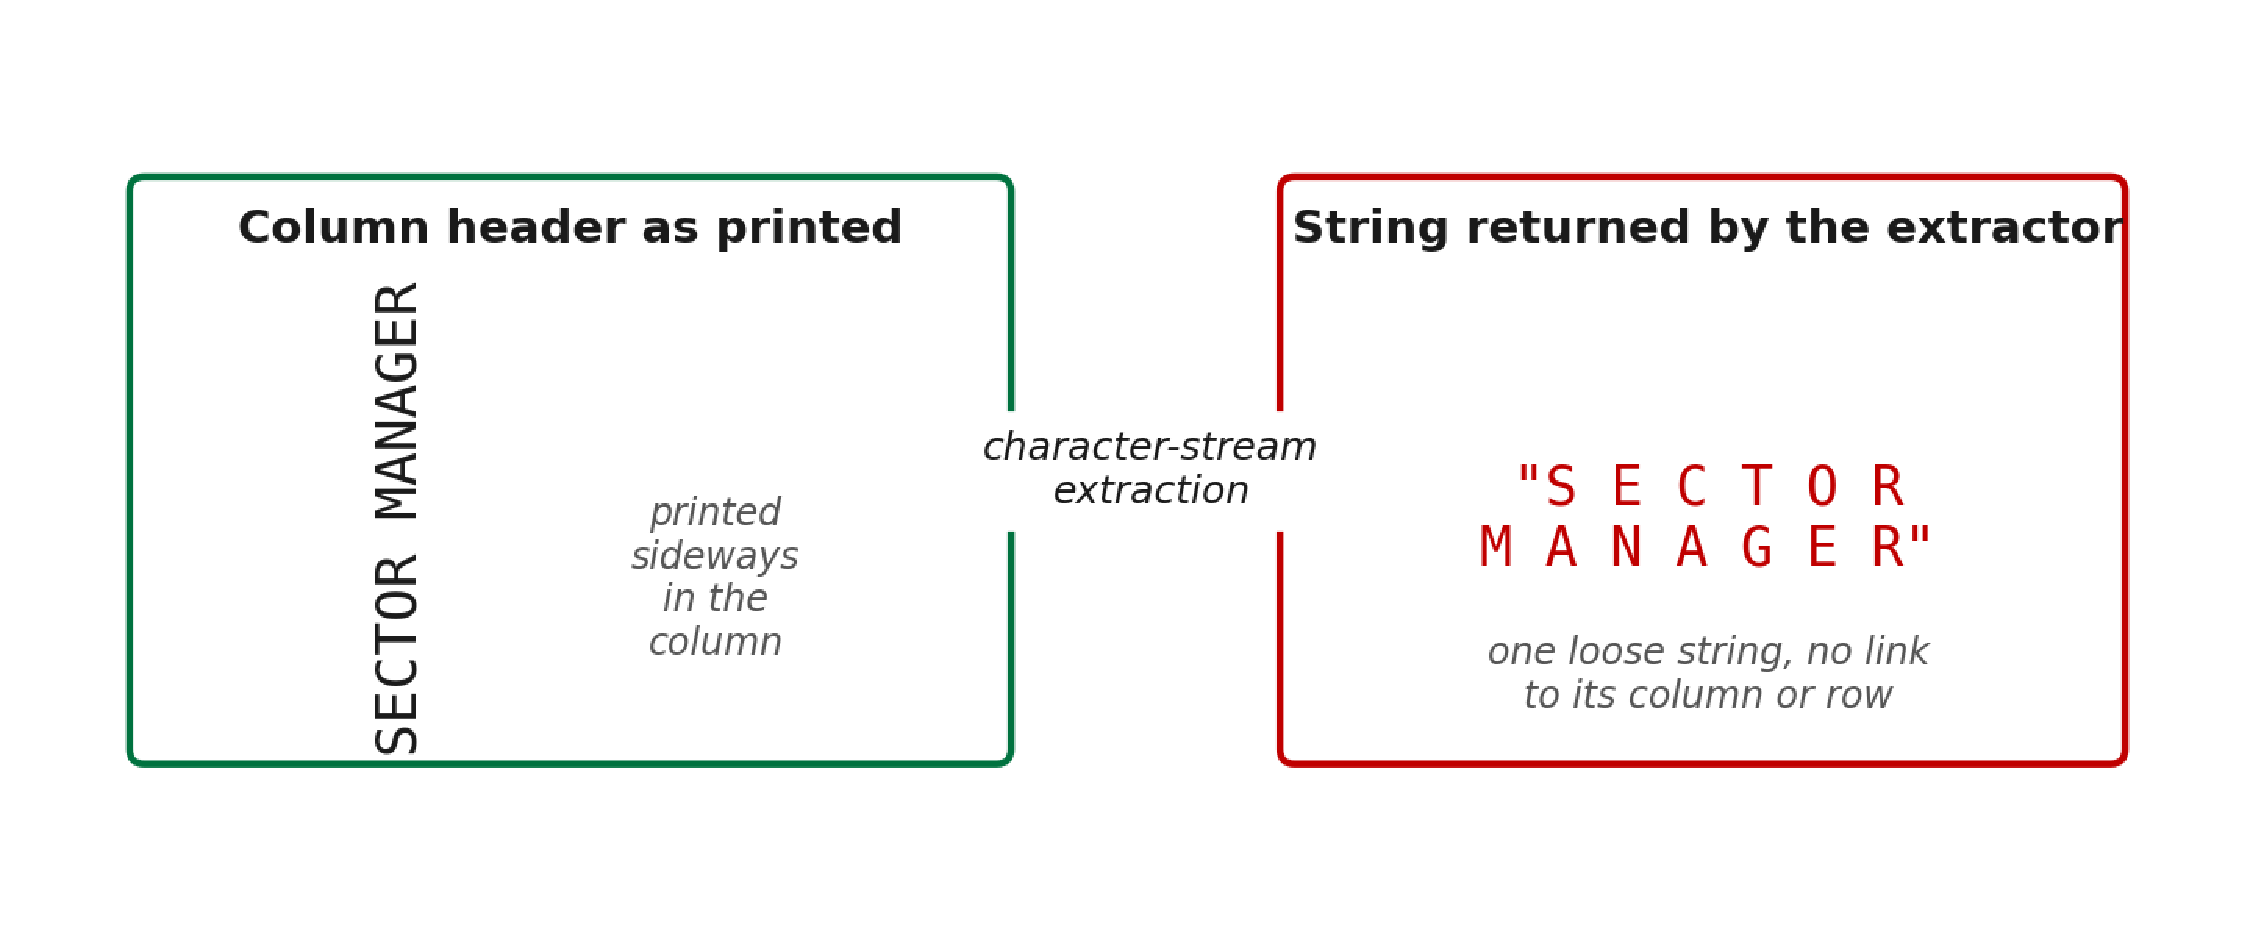
\includegraphics[width=0.92\textwidth]{figures/fig2_rotated_headers.pdf}
\caption{Column headers as printed, rotated through ninety degrees, beside the text an
extractor returns for the same region. The header row is not recoverable as a table header.}
\label{fig:rotatedheaders}
\end{figure}

\subsection{Rotated Column Headers}

The headers and the text an extractor returns for them are shown side by side in Figure~\ref{fig:rotatedheaders}.

Headers for roles are printed vertically. When the standard word extraction is used, they appear just as plain words with usual coordinates, which means that nothing is known about their rotation and the horizontal position of the word corresponds to the narrow strip of the rotated text rather than the whole column underneath it. Therefore, in order to attribute any code to some role, header words have to be clustered by their horizontal position and each cell should be associated with the nearest header cluster. The problem occurred somewhere in the middle of the document: some pages have headers only once and the table continues further without them. These pages have codes but no headers, so attribution fails unless the last seen headers are used instead.

\subsection{Fused Footnote Digits and Authority Codes}

Figure~\ref{fig:fusedfootnote} shows a code and its footnote marker as printed, alongside the fused token that results when the size difference between them is disregarded.

The footnote markers are encoded as the superscripts adjacent to the authority code. After extraction, if the code A and the footnote 3 occur, the string “A3” is produced, which visually cannot be distinguished from the correct level-bearing code “A3.” The distinction can be made only on the basis of the vertical offset of the digits from the baseline and the difference in font sizes between the digit and the letter. Superscripts appear at higher offsets and in smaller fonts, and the rule was established experimentally based on real-life examples of characters, not on intuitive assumptions, since the offsets are small, and an intuitively guessed threshold would result in a significant number of misclassifications.
Another flaw impacted the informed marker. Since the marker consisted of the parenthesized character i, it could be detected by the string “(i)” in the text. However, on a real-life page, this marker consists of five separate characters, so nothing matched. Before this problem was discovered, of the 276 records in an early version of the extraction, 174 included the informed marker inside the printed document that had no impact on the extracted data. This flaw remained undetected until the output involved record comparison with the page. It can be explained by the fact that there is an additional Authority code when flattened produces the same string “I”.

\begin{figure}[htbp]
\centering
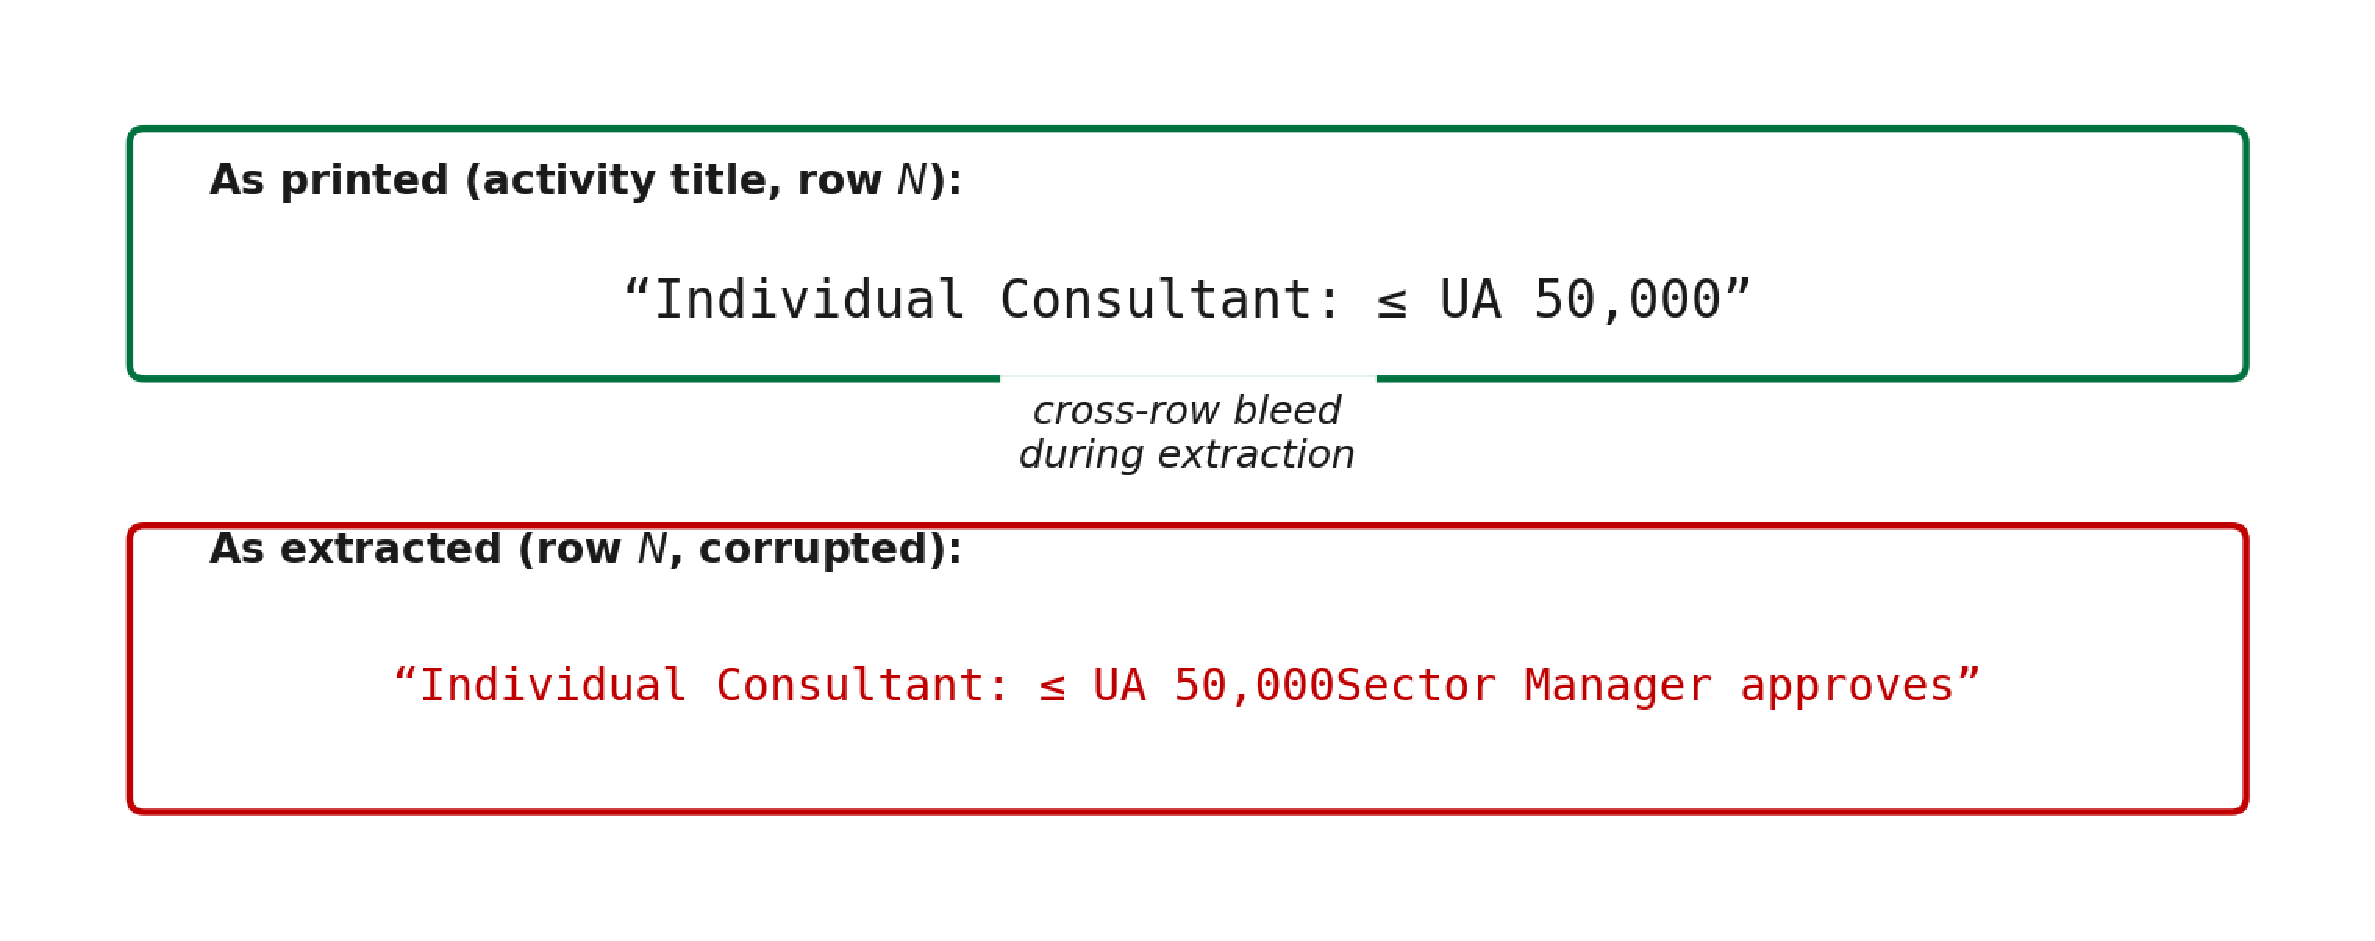
\includegraphics[width=0.92\textwidth]{figures/fig2_title_corruption.pdf}
\caption{An activity title as printed, and the corrupted string produced when text from an
adjacent row bleeds into it during extraction.}
\label{fig:titlecorruption}
\end{figure}

\subsection{Cross-Row Text Bleeding and Title Corruption}

Figure~\ref{fig:titlecorruption} pairs a printed title with the corrupted string extracted for the same activity.

The activity titles can consist of several lines, so a line of the title of one activity can be closer to the row of another activity in a dense table. In such situations, the title is associated with the wrong activity. Therefore, both activities are valid by themselves : one of them contains an overly short title, while the other is overly long, and there is nothing indicating that an error has occurred.
At its worst, the problem occurred in roughly one-quarter of the records generated by a preliminary version of the parser. This was resolved through the use of a system where in title attachment depended on the parse state rather than just proximity, utilizing the following three criteria: (1) is there currently an open task, (2) does the open task's text end in a period, and (3) does the line have authority codes when the open task already has them? After implementing these rules, the sole outstanding case occurred in the entire set of records for activity 2.222.1, a documented exception rather than an automatic acceptance.

\subsection{Split Rows in the Non-Sovereign Operations Chapter}
\label{sec:splitrows}

With the introduction of the Non-Sovereign Operations chapter, as well as the need to define scope after the initial parsing of the text, a layout exception was introduced wherein a single logical row was sometimes laid out as two separate rows, with the authority codes appearing a bit below the activity text. The first attempt at correction consisted of simply merging any two vertically contiguous bands separated by less than some tolerance level. A check done before implementation showed 1,614 candidates mergers in the document, but many of them were incorrect and would have merged unrelated activities. This general solution was therefore dismissed, and a more limited one adopted whereby only a band containing nothing other than authority codes was merged, a strong indicator that it was part of the row above it.

\begin{figure}[htbp]
\centering
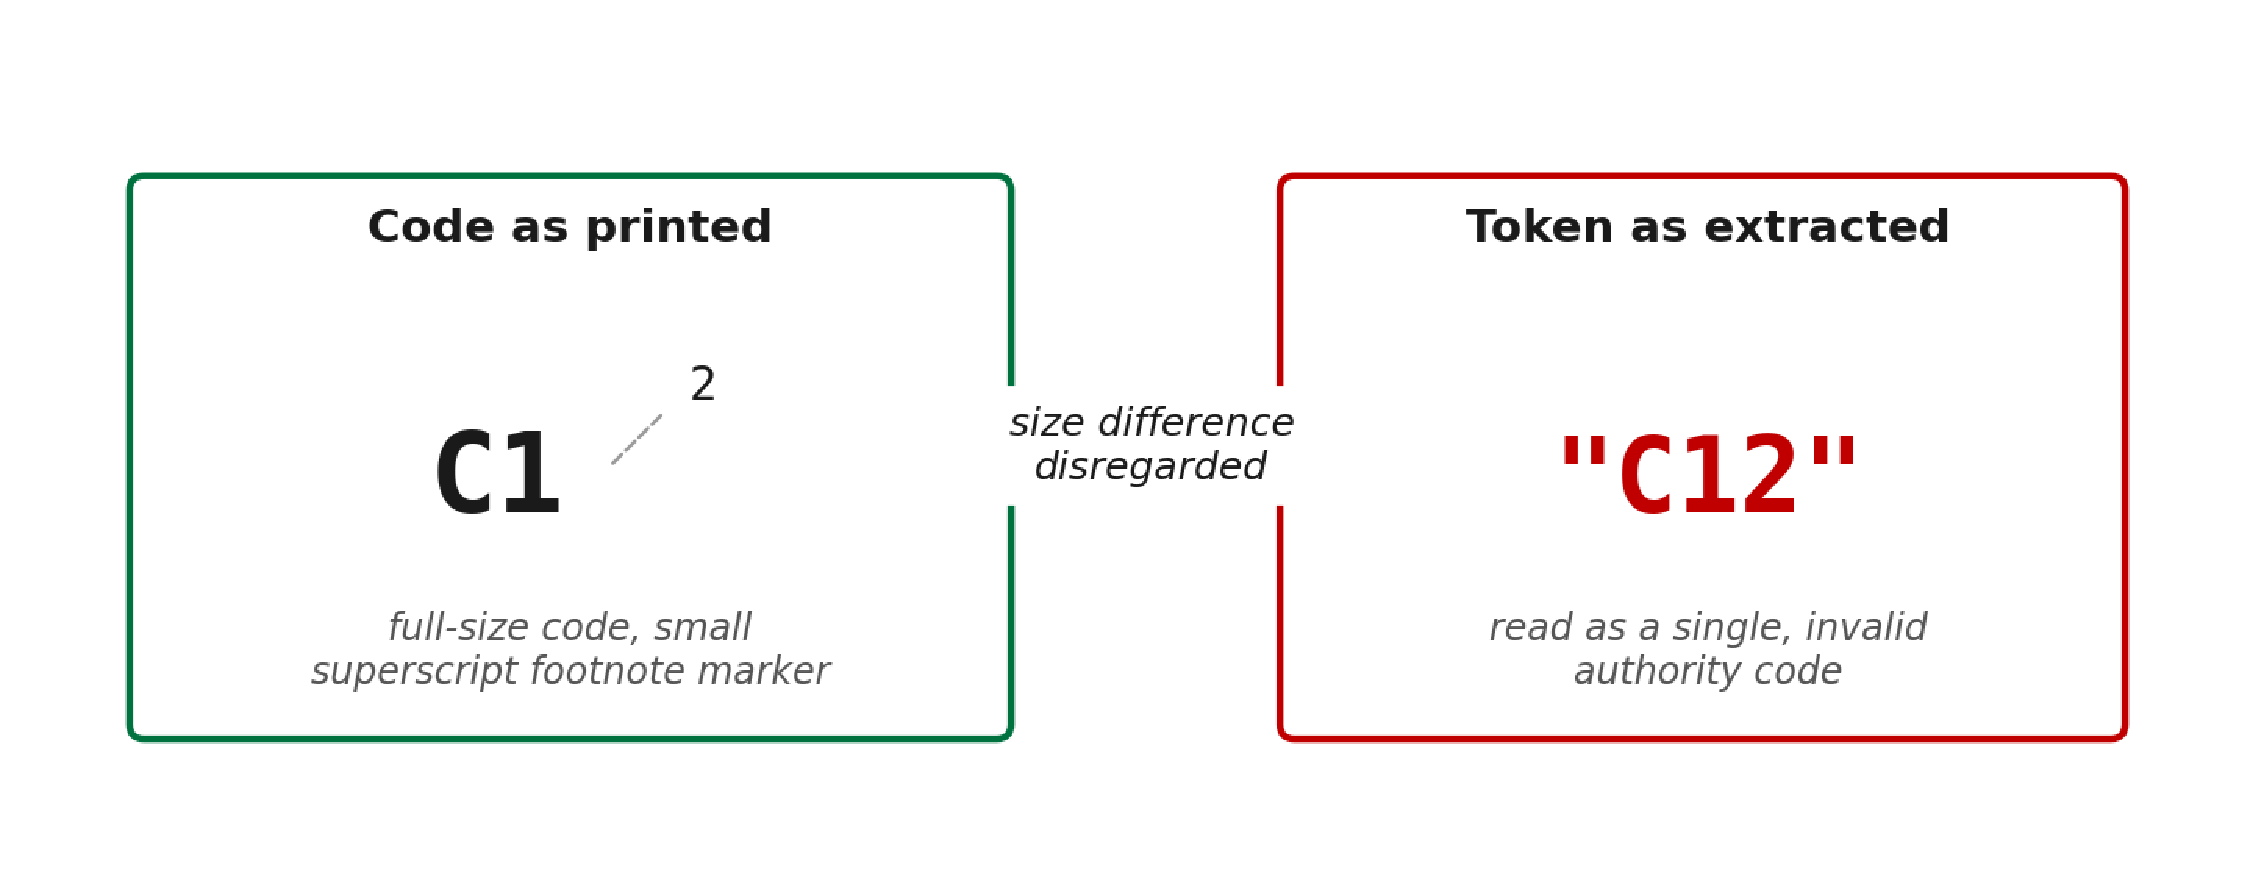
\includegraphics[width=0.78\textwidth]{figures/fig2_fused_footnote.pdf}
\caption{An authority code printed beside a superscript footnote marker, and the fused token
produced when the size difference between them is disregarded.}
\label{fig:fusedfootnote}
\end{figure}

\subsection{Consolidated Data Issues Summary}

Table~\ref{tab:issues} consolidates the defects described above, each paired with the stage of the pipeline that addresses it.

\begin{longtable}{|p{0.24\textwidth}|p{0.30\textwidth}|p{0.34\textwidth}|}
\caption{Consolidated summary of extraction issues found in the source document.}\label{tab:issues}\\
\hline
\rowcolor{myblue}\textcolor{white}{\textbf{Issue}} & \textcolor{white}{\textbf{Effect if unhandled}} & \textcolor{white}{\textbf{Resolution}} \\
\hline
\endfirsthead
\hline
\rowcolor{myblue}\textcolor{white}{\textbf{Issue}} & \textcolor{white}{\textbf{Effect if unhandled}} & \textcolor{white}{\textbf{Resolution}} \\
\hline
\endhead
Rotated column headers & Codes cannot be attributed to roles. & Cluster header text by horizontal position; carry the header set forward across continuation pages. \\ \hline
Missing headers on continuation pages & Whole pages of responsibilities lost. & Reuse the last seen header set until a new one appears. \\ \hline
Footnote digits fused with codes & Codes misread; footnote qualifications lost. & Separate by measured vertical offset and font size of the character. \\ \hline
Informed marker not matched & Informed parties absent from the majority of records. & Match the marker as the separate characters it is actually rendered as. \\ \hline
Title bleeding across rows & Titles attached to the wrong activity; free-text search degraded. & Conditional attachment based on parse state, terminating punctuation, and code presence. \\ \hline
Split rows in the NSO chapter & Responsibilities detached from their activity. & Merge a band only when it consists entirely of authority codes. \\ \hline
Hierarchy from string prefixes & Two of four hierarchy levels silently wrong. & Derive parentage from explicit parent fields and process arithmetic. \\ \hline
Cross-reference rows & Activities reported as having no responsibilities. & Extract references, expand ranges, and follow pointers at query time. \\ \hline
\end{longtable}

\section*{Conclusion}
\addcontentsline{toc}{section}{Conclusion}
DAM can be seen as a well-written document for humans, and as an adversarial artifact for the parser, given that all the structural features that this artifact has can be conveyed using its structure. The problems presented in this chapter do not constitute edge cases. Rather, they together impact all the components in the answer that the parser should provide : the hierarchy, roles, titles, and informed parties. Furthermore, this chapter presents a methodology that can be applied in practice. None of these problems were detected using code inspection or by inferring what the parser was supposed to output. Rather, each problem was detected by collecting the output and comparing it against the corresponding page. This methodology continues in all subsequent parts of this thesis, as discussed in Chapter 3.
\chapter{Data Engineering Pipeline and Knowledge Graph Construction}
\label{ch:pipeline}
\minitoc

\section*{Introduction}
\addcontentsline{toc}{section}{Introduction}

This chapter details the transformation of the source document into queryable data. It discusses the selected processing environment, outlines the design of the extraction pipeline, and explicates the transformations implemented at each stage. Additionally, it presents the validated node set generated and the knowledge graph constructed from it, concluding with an evaluation of the pipeline's performance and its remaining limitations.

\section{Processing Environment}

Before describing the pipeline itself, it is worth justifying the kind of pipeline it is.
Three choices were made before any extraction rule was written: a deterministic, rule-based
approach over a learned one, a single-process program over a distributed framework, and a
specific set of libraries chosen against the constraints of Table~\ref{tab:constraints}.

\subsection{Motivation for a Deterministic, Rule-Based Pipeline}

An alternative strategy for addressing this extraction challenge involves training a model by annotating a selection of pages to classify text regions and subsequently generalizing from this information. However, this approach was ultimately dismissed for practical reasons prior to any principled considerations. Specifically, the absence of annotated data posed significant hurdles, as the effort required to produce sufficient annotations for a single seventy-nine-page document would have outweighed the efforts involved in crafting a set of rules, all while complicating verifiability.

Verifiability serves as the foundational rationale for adopting a rule-based approach. Rules derived from measured character geometry can be readily verified against the originating page. In instances of failure, such discrepancies can be inspected closely, and the necessary corrections are localized. Conversely, a learned region classifier that misinterprets a single table offers no comparable insight into its decision-making process. In documents where errors are subtle and plausible, the ability to elucidate the reasoning behind a character's interpretation holds greater value than the enhanced flexibility that a learned approach might provide.

\subsection{Why Not a Distributed Processing Framework}

Distributed frameworks, such as Apache Spark, are typically employed when data processing demands exceed the capabilities of a single machine. However, this particular scenario is not one of those cases. The complete document is only a few megabytes, and the subset processed yields 327 records, with a full reconstruction of the knowledge base requiring approximately fifteen to twenty seconds on an average laptop.

Implementing a distributed framework would introduce unnecessary complexities, such as an execution model, cluster configuration, and serialization boundaries, which are irrelevant to this problem. The primary challenge lies in the interpretative aspect, specifically in discerning the meanings of characters rather than in the rapid processing of numerous characters. Consequently, the pipeline is structured as a single-pass, single-process program, which is best suited for this task and facilitates inspection of intermediate outputs during development.

\subsection{Libraries Selected for Extraction, Validation and Modelling}

Extraction is facilitated by pdfplumber\citep{pdfplumber}, which provides detailed information about characters and words, including their coordinates, font names, and sizes. This character-level access is essential, as the superscript rule discussed in Chapter 2 relies on the vertical offset and size of individual characters, making ware-level output insufficient.

The node model is established using Pydantic\citep{pydantic_docs}, ensuring that structural expectations are strictly enforced during construction. Consequently, any record that omits a required field or contains an authority code outside the recognized set will fail promptly, preventing issues from arising later in the graph.

\section{Pipeline Design}

With the environment settled, the pipeline itself has a shape worth laying out: how many
stages it has, what each one hands to the next, and how the code implementing it is
organised into modules.

\subsection{Global Architecture}

The process pipeline is made up of eight consecutive processes, where each process takes input from its previous process, and each process can be inspected independently. The raw characters get converted to physical rows, the physical rows are grouped into task blocks, the task blocks are cleaned and enriched with geometric and role-based data, and finally, they are arranged into validated records.
Figure~\ref{fig:pipeline} shows the pipeline end to end, and it is worth reading it as a
progressive narrowing of interpretation rather than as a sequence of transformations. At
the left-hand edge the input is a stream of glyphs with coordinates, carrying no notion of
a row, a cell, an activity or a role: the PDF format records where ink was placed, not what
the ink means. At the right-hand edge the output is a set of validated records in which
every responsibility is an explicit assertion that a named role holds a named obligation
over a named activity. Every stage in between recovers exactly one layer of structure that
the printed page expresses visually and the file itself does not encode.

The ordering is not arbitrary, and the stages are not independent. Each one consumes an
abstraction the previous stage established and would be meaningless without it: codes
cannot be separated from footnote markers before there are cells to inspect, cells cannot
be attributed to roles before the rotated column headers have been clustered into columns,
and no activity can be assembled before its block boundaries are known. This dependency is
the reason the pipeline is deterministic and staged rather than a single extraction pass.
A failure at any stage is therefore localised to that stage and inspectable in isolation,
which is what made the defects catalogued in Chapter~\ref{ch:datasource} diagnosable at
all.

\begin{figure}[htbp]
\centering
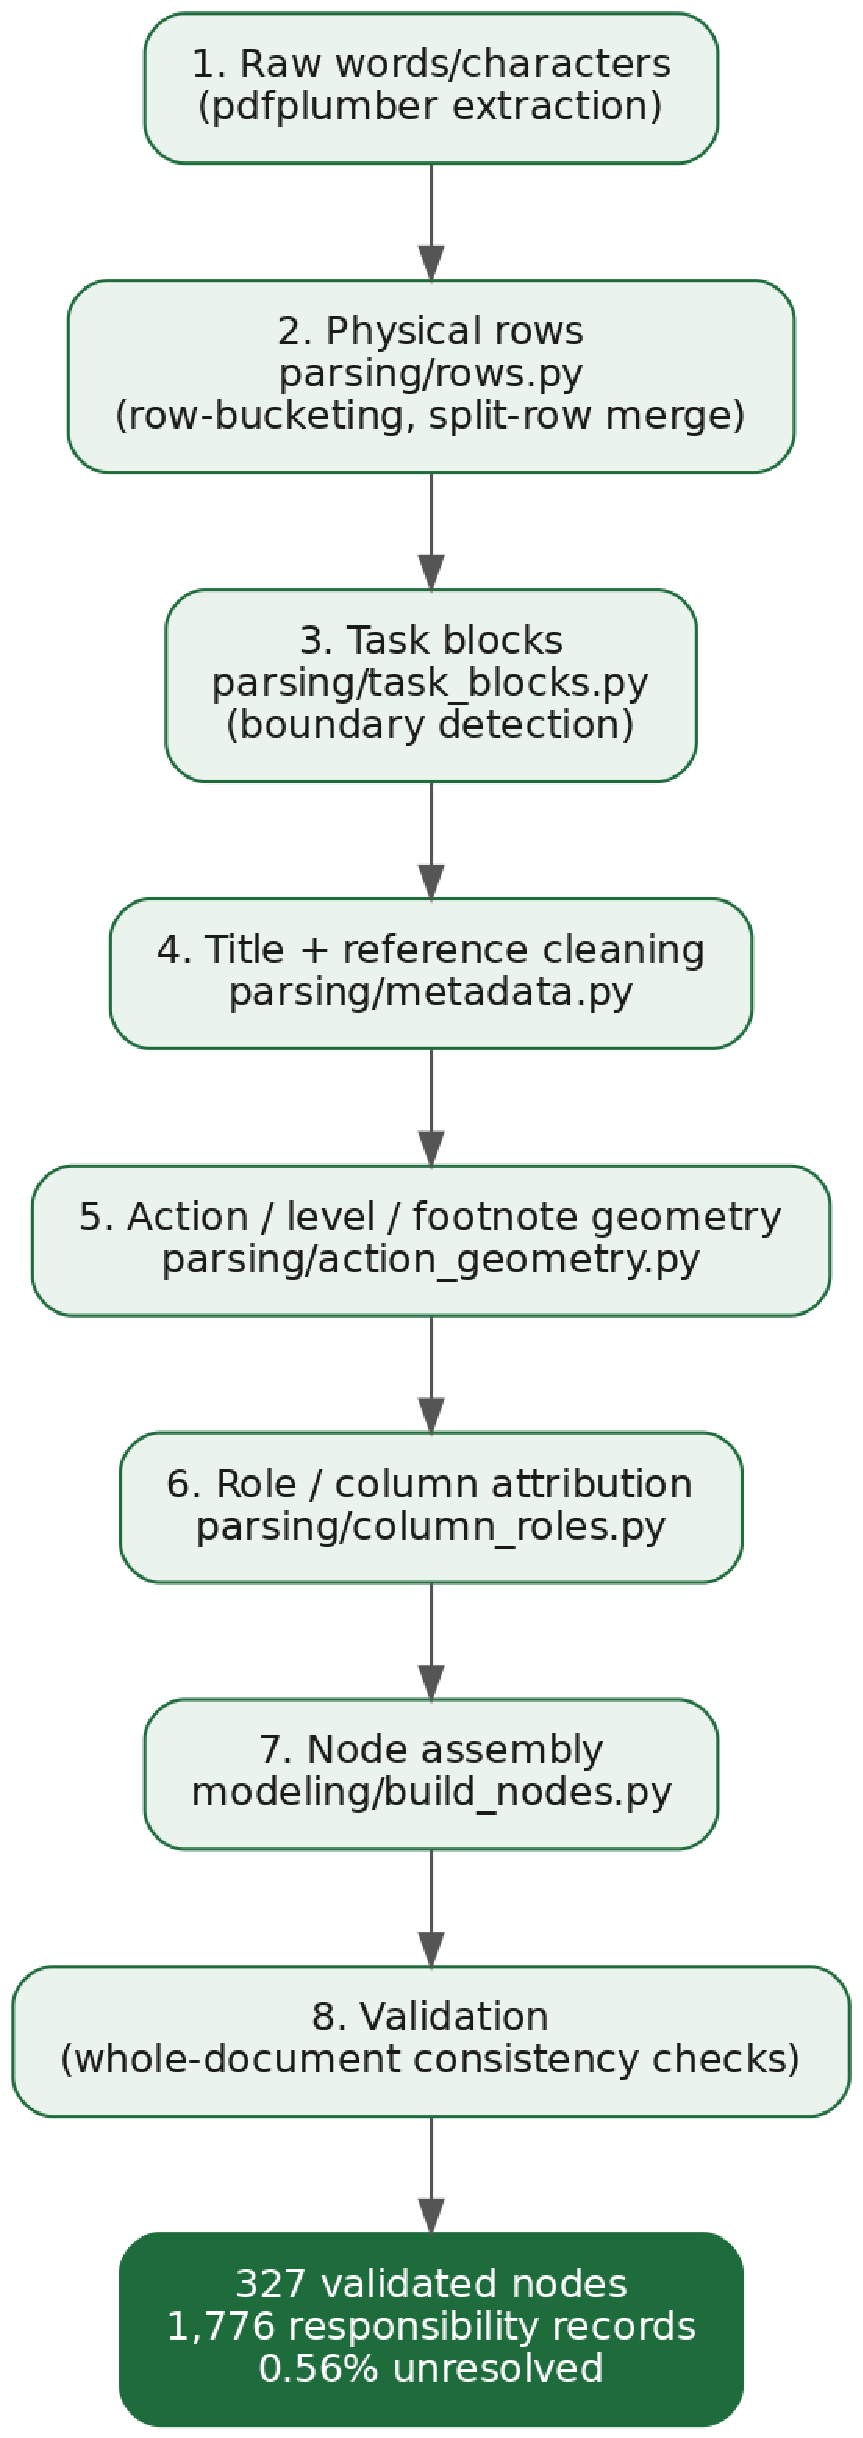
\includegraphics[width=0.94\textwidth,height=0.88\textheight,keepaspectratio]{figures/fig2_pipeline.pdf}
\caption{Eight-stage data engineering pipeline, from raw PDF extraction to a validated node set.}
\label{fig:pipeline}
\end{figure}

Table~\ref{tab:stages} names each stage, states what it does, and records why it exists at all, since several of them were added only after a specific defect made their absence visible.

\begin{longtable}{|p{0.045\textwidth}|p{0.19\textwidth}|p{0.32\textwidth}|p{0.30\textwidth}|}
\caption{Stages of the data engineering pipeline, with the motivation for each.}\label{tab:stages}\\
\hline
\rowcolor{myblue}\textcolor{white}{\textbf{\#}} & \textcolor{white}{\textbf{Name}} & \textcolor{white}{\textbf{Function}} & \textcolor{white}{\textbf{Why it exists}} \\
\hline
\endfirsthead
\hline
\rowcolor{myblue}\textcolor{white}{\textbf{\#}} & \textcolor{white}{\textbf{Name}} & \textcolor{white}{\textbf{Function}} & \textcolor{white}{\textbf{Why it exists}} \\
\hline
\endhead
1 & Raw extraction & Characters and words with coordinates, fonts, and sizes are read from the PDF. & Page-level text extraction discards the geometry on which every later stage depends, so extraction had to be character-level from the outset. \\ \hline
2 & Row reconstruction & Words are grouped into physical rows by vertical alignment, with split rows merged where the merge is provably safe. & Activities in the Non-Sovereign Operations chapter are printed across two physical rows, and without merging they were parsed as two unrelated fragments. \\ \hline
3 & Task block detection & Rows are grouped into task blocks, and boundaries between consecutive activities are determined. & A title wrapping past its own identifier row was being claimed by the following activity, which silently attached responsibilities to the wrong task. \\ \hline
4 & Title and reference cleaning & Titles are normalised, cross-references are extracted and expanded, footnote digits are stripped from title text. & Roughly a quarter of titles carried embedded reference phrases or stray digits, which corrupted the search index and made free-text resolution unreliable. \\ \hline
5 & Geometric attribution & Authority codes are separated from footnote markers by character geometry, and levels are attached. & A code and a footnote marker are both a letter beside a digit; only font size and vertical offset distinguish them, so fusing the two inverted the meaning of the cell. \\ \hline
6 & Role attribution & Codes are matched to roles by horizontal alignment with clustered, rotated column headers. & Column headers are printed rotated through ninety degrees and are not recoverable as table headers, so columns had to be reconstructed from header coordinates. \\ \hline
7 & Node assembly & Enriched blocks are validated against the schema and merged with the chapter and process skeleton. & Enforcing the schema at construction makes a malformed record fail immediately, rather than surfacing later as a wrong answer to a user. \\ \hline
8 & Validation & Whole-document consistency checks are run across the assembled node set. & Per-record validity does not imply document-level coherence: orphaned identifiers and unresolved references are only visible once the full set exists. \\ \hline
\end{longtable}

\subsection{Data Flow and Modular Organisation}

The process is performed in each individual module with well-defined boundaries such that if an error occurs, it will be easier to pinpoint exactly where it occurred based on the output of one particular stage as opposed to following the execution throughout the whole program. This factor had great significance throughout the development process because whenever an incorrect output came out, the first thing to consider was which stage produced it.

Modules for parsing take care of rows, action blocks, metadata, geometry of action, column definitions, and text cleaning. Modules for modelling handle nodes, structural backbone, graph, and caching. The schema lives in a separate module, which is dependent on both but depends on none of the two.

\section{Data Ingestion}

The ingestion process deals with each page of the document individually. Characters and their locations and font metrics, as well as words with their bounding boxes are extracted from every single page. These two granularities are saved because the row construction needs word granularity, and the superscript rule is based on the character granularity.

References are extracted independently from other pages of the same document. The legend of authority codes is converted into a structured file that describes the full code, its hierarchy level and the meaning. This reference is checked against the schema and seventeen entries are loaded successfully. Abbreviations are extracted as a glossary. The glossary needed a special approach due to the facts that some entries break a line, some rows are section headings but not the definitions and the term and its definition are sometimes placed with a fractional difference in point. Therefore, row grouping is done with the same tolerance as elsewhere in the processing.

\section{Document Processing and Normalisation}

Stages two through six of Table~\ref{tab:stages} are covered here: the point where raw
characters become rows, rows become task blocks, and blocks are cleaned and enriched enough
for a schema to accept them. This is also where most of the defects catalogued in
Chapter~\ref{ch:datasource} are addressed directly, one subsection per family of defect.

\subsection{Row Reconstruction}

Words are arranged into lines through grouping of their vertical coordinates. The reason for tolerance is that text that may appear on the same visual line is normally not placed on identical coordinates. Where the chapter Non-sovereign operations splits a logical line into two lines, these lines are combined into one only when the specific condition described in Chapter 2 applies. That is, the lower line consists of authority codes alone.

\subsection{Task Block Detection}

Blocks then come out of rows in such a way that each block represents an activity. The boundary detection turned out to be the most iterative part of the process as the visual cue that denotes a boundary was unreliable. There were three different cues considered: (1) whether there is an open task, (2) whether the open task ends on a full stop, and (3) whether there is any new row with authority codes while there are codes for the current open task. Of these three cues, the third one appears to be the most reliable one.

\subsection{Title and Reference Cleaning}

Normalization of titles is achieved by stripping footnote digits, compressing whitespace, and stripping references that would have been incorporated as noise in the title. Extraction of references is concentrated in one function used by all pathways that deal with titles or notes. The current scheme contrasts with the original design that had two different but conflicting implementations, one of which could handle the reference pattern while the other could not.

\subsection{Geometric Attribution of Authority Codes}

Codes of authority are found in each row and are distinguished from footnote indicators according to the character-level rule stated in Chapter 2. Level digits belonging to the codes remain intact as part of the code, but superscripted digits are entered independently as footnote numbers for that responsibility.

\subsection{Role Attribution}

The enriched blocks are put together in such a way that the records follow the required schema and they get coupled with a structural skeleton that contains the chapter nodes and process nodes, since these nodes are containers for the records and not emitted as activities by the table parser.

The parentage is defined explicitly and not by the structure of the identifiers. There is a pointer to the parent node inside each record and the hierarchy is built using these pointers. In an older version of the system, the children of a node were defined based on the structure of the identifier and it worked well only for two of the four levels but not for the other two levels. This problem was detected only when the threshold variants started appearing in the identifier space and the grandchildren were clashing with the children under the same prefix.

The indicators in Table~\ref{tab:quality} are the measured state of the node set after construction, and they are the figures against which the pipeline's adequacy is judged.

\begin{longtable}{|p{0.52\textwidth}|p{0.34\textwidth}|}
\caption{Data quality indicators after node construction.}\label{tab:quality}\\
\hline
\rowcolor{myblue}\textcolor{white}{\textbf{Indicator}} & \textcolor{white}{\textbf{Value}} \\
\hline
\endfirsthead
\hline
\rowcolor{myblue}\textcolor{white}{\textbf{Indicator}} & \textcolor{white}{\textbf{Value}} \\
\hline
\endhead
Structured records produced & 327 \\ \hline
Responsibility entries extracted & 1,776 \\ \hline
Distinct roles identified & 131 \\ \hline
Unresolved role entries & 10 (0.56\%) \\ \hline
Average responsibilities per record & 5.48 \\ \hline
Records with no direct responsibilities & 29.63\% \\ \hline
Cross-references captured & 14 \\ \hline
Responsibility entries carrying footnote references & 113 (6.36\%), across 44 records \\ \hline
Residual title corruption & 1 record (2.222.1) \\ \hline
\end{longtable}

\subsection{Geometric Tolerances}
\label{sec:geotolerances}

Several pipeline stages reason about position and size rather than about text, because the
distinctions they draw are not present in the character stream at all. Those stages are
governed by the tolerances in Table~\ref{tab:geoparams}, stated in PDF user-space units,
where one unit is $1/72$ of an inch. The values are recorded here because without them the
extraction is not reproducible: the same source document processed with different tolerances
yields a different node set.

\begin{longtable}{|p{0.26\textwidth}|p{0.09\textwidth}|p{0.51\textwidth}|}
\caption{Geometric tolerances governing extraction, in PDF user-space units.}\label{tab:geoparams}\\
\hline
\rowcolor{myblue}\textcolor{white}{\textbf{Tolerance}} & \textcolor{white}{\textbf{Value}} & \textcolor{white}{\textbf{What it separates}} \\
\hline
\endfirsthead
\hline
\rowcolor{myblue}\textcolor{white}{\textbf{Tolerance}} & \textcolor{white}{\textbf{Value}} & \textcolor{white}{\textbf{What it separates}} \\
\hline
\endhead
Body text minimum size & $8.0$ & Characters at or above this size are body text. Below it, a character is a candidate footnote marker rather than content. \\ \hline
Footnote digit maximum size & $4.0$ & A trailing digit at or below this size is treated as a footnote reference and stripped from the cell. \\ \hline
Row band padding & $1.0$ & Vertical tolerance when collecting the characters and words belonging to one printed row. \\ \hline
Row merge maximum gap & $5.0$ & Two vertically adjacent row bands closer than this may be merged into a single logical row. \\ \hline
Column alignment tolerance & $2.0$ & Horizontal distance within which a cell is considered aligned to a column centre. \\ \hline
Tight cluster gap & $3.0$ & Characters separated by less than this belong to the same header cluster. \\ \hline
Column merge gap & $14.0$ & Two header clusters closer than this are treated as one column rather than two. \\ \hline
Subgroup tolerance & $0.6$ & Vertical agreement required for header fragments to form one subgroup. \\ \hline
Subgroup minimum gap & $1.5$ & Separation below which two candidate subgroups are not distinguished. \\ \hline
Decoration gap maximum & $8.0$ & Distance beyond which an adjacent glyph is ruled out as decoration attached to a code. \\ \hline
Spaced-word gap maximum & $6.0$ & Gap below which adjacent single letters are read as letter-spaced prose rather than as standalone codes. \\ \hline
Glossary title minimum size & $20$ & Font size at or above which a glossary line is a heading rather than an entry. \\ \hline
Glossary top merge tolerance & $3.0$ & Vertical tolerance when joining a wrapped glossary definition to its term. \\ \hline
\end{longtable}

Two of these tolerances resolve ambiguities that no single test settles on its own.

The footnote-digit rule is size-based, and size alone produces false positives. Department
codes such as \texttt{PGCL.1}, \texttt{FIFC.4} and \texttt{FITR.2} also end in a digit, and
that digit belongs to the code. The rule therefore carries a second, independent condition:
the character preceding the digit must not be a period. The two tests are needed together
because the same code was observed rendering its digit at normal size on some pages and at
the reduced footnote size on others, so size is not a reliable discriminator by itself.

The spaced-word tolerance separates a genuine authority code from letter-spaced prose. A
single capital letter standing alone in a row may be an authority code, or it may be one
glyph of a title that the renderer has spaced out character by character, as in
\texttt{A p p r a i s a l}. A real code is followed either by the gap to the next table
column or by nothing at all, so adjacency below $6.0$ units to another single-letter word
identifies the second case. Authority codes themselves are recognised by the pattern
\texttt{\^{}[ICRA]\textbackslash d*\$}, one of the four letters with an optional level digit.

\begin{figure}[htbp]
\centering
% ---------------------------------------------------------------
% PLACEHOLDER — replace with an annotated page crop showing the
% geometry: column header clusters, the alignment band for one
% column, a normal-size code beside a reduced-size footnote digit.
% Suggested filename: figures/fig3_geometry_annotated.png
% ---------------------------------------------------------------
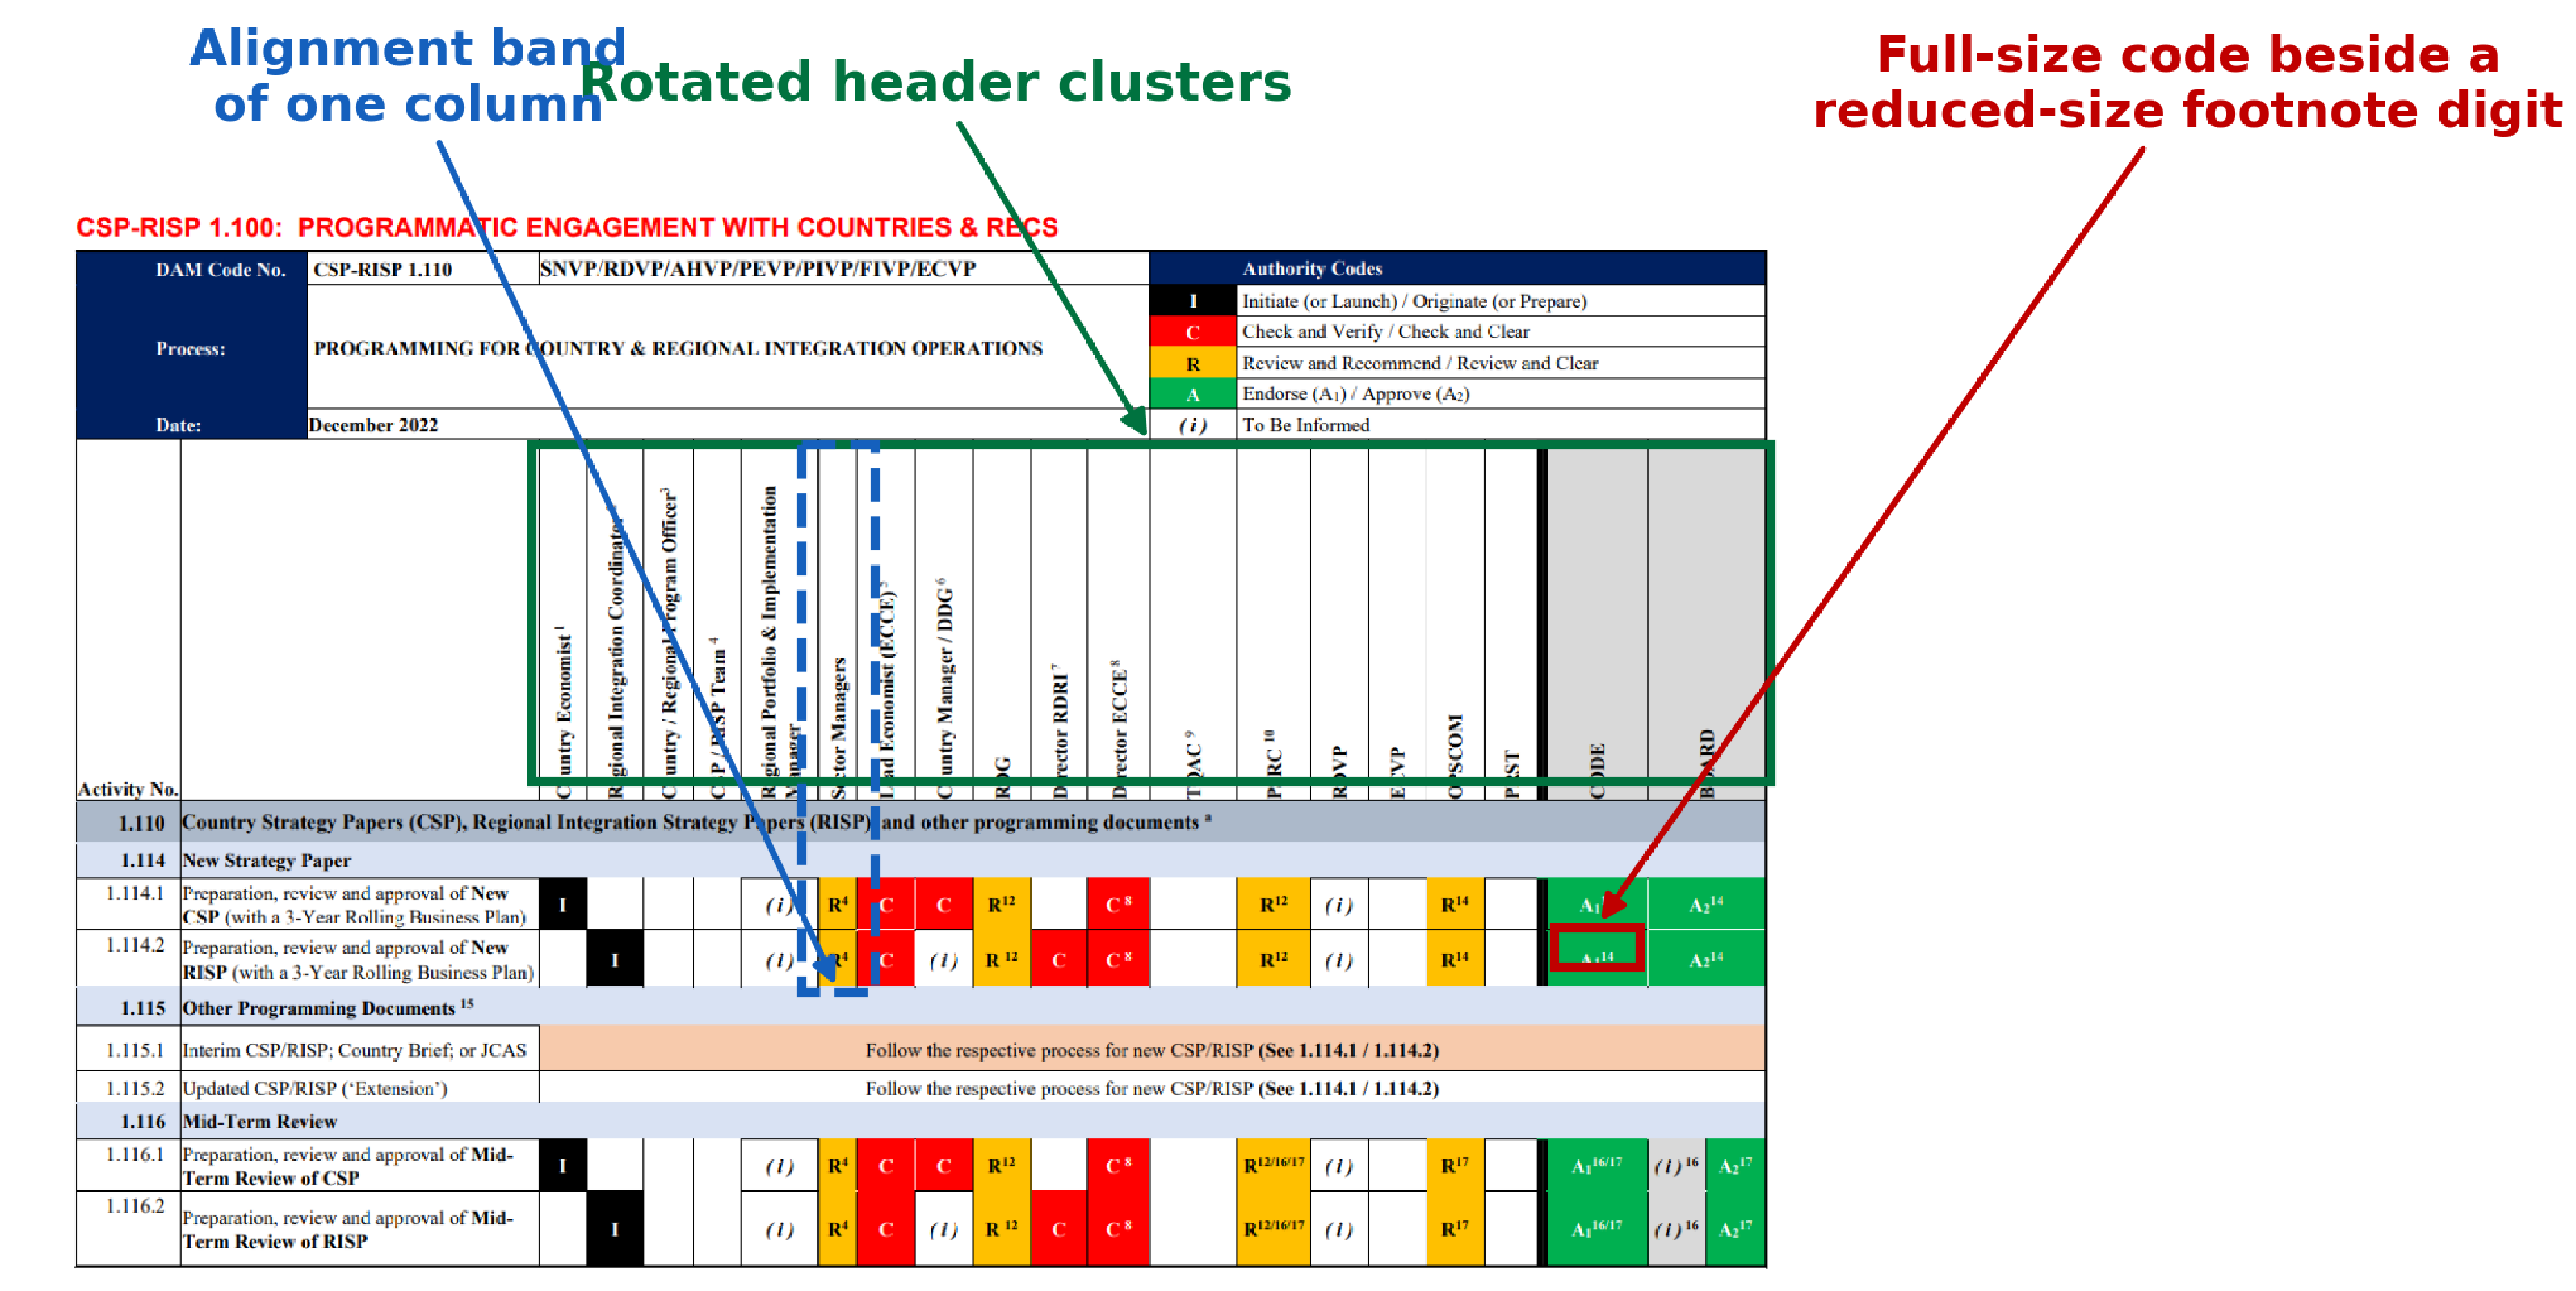
\includegraphics[width=0.95\textwidth]{figures/fig3_geometry_annotated.pdf}
\caption{A DAM table region annotated with the geometric quantities used during extraction:
rotated header clusters, the horizontal alignment band of one column, and a full-size
authority code beside a reduced-size footnote digit.}
\label{fig:geoannotated}
\end{figure}

Figure~\ref{fig:geoannotated} shows these quantities on a real page region.

\section{Knowledge Graph Modelling}

The pipeline's final output is a validated set of nodes, but a set on its own cannot answer
a relational question such as who approves an activity. That is why the nodes are loaded
into a graph rather than kept flat, with the graph's nodes and edges defined next, along
with what the assembled structure looks like in aggregate.

\subsection{Why a Graph}

The valid set of nodes could have been modeled as either relational tables or as a flat set of documents\citep{hogan2021kg}. The graph was chosen since the queries posed to the system are relational in nature. For instance, the query "Who approves this activity" translates into traveling in the graph from the activity node via edges of a certain kind, while "which activities does this role approve" amounts to traveling the opposite way in the graph. In both instances, the operation performed is a single one on a graph, unlike join or scan on a flat structure.

A directed multigraph is used instead of a simple graph since one role can hold multiple responsibilities for the same activity. That is why two nodes will be linked with multiple edges, each carrying its unique authorization code and references to the footnote.

\subsection{Node and Edge Schema}

The graph contains two kinds of node. Activity nodes correspond one-to-one with the 327 structured records. Role nodes correspond to the 131 distinct roles. Edges carry the relationships between them.

Table~\ref{tab:edges} sets out the edge types the graph carries and what each one asserts.

\begin{longtable}{|p{0.24\textwidth}|p{0.24\textwidth}|p{0.42\textwidth}|}
\caption{Edge types in the knowledge graph.}\label{tab:edges}\\
\hline
\rowcolor{myblue}\textcolor{white}{\textbf{Edge type}} & \textcolor{white}{\textbf{From $\rightarrow$ To}} & \textcolor{white}{\textbf{Meaning}} \\
\hline
\endfirsthead
\hline
\rowcolor{myblue}\textcolor{white}{\textbf{Edge type}} & \textcolor{white}{\textbf{From $\rightarrow$ To}} & \textcolor{white}{\textbf{Meaning}} \\
\hline
\endhead
\texttt{contains} & Activity $\rightarrow$ Activity & Hierarchical containment: chapter to process, process to task, task to child task or threshold variant. \\ \hline
\texttt{responsible\_for} & Role $\rightarrow$ Activity & A recorded responsibility, carrying the authority code, its level, and any footnote references. \\ \hline
\texttt{references} & Activity $\rightarrow$ Activity & A cross-reference extracted from the activity's own text, including ranges expanded to their members. \\ \hline
\end{longtable}

Figure~\ref{fig:graph} shows a representative excerpt, centred on activity 3.111, in which the containment edge from the parent process and the individual responsibility edges to each role are both visible.

\begin{figure}[htbp]
\centering
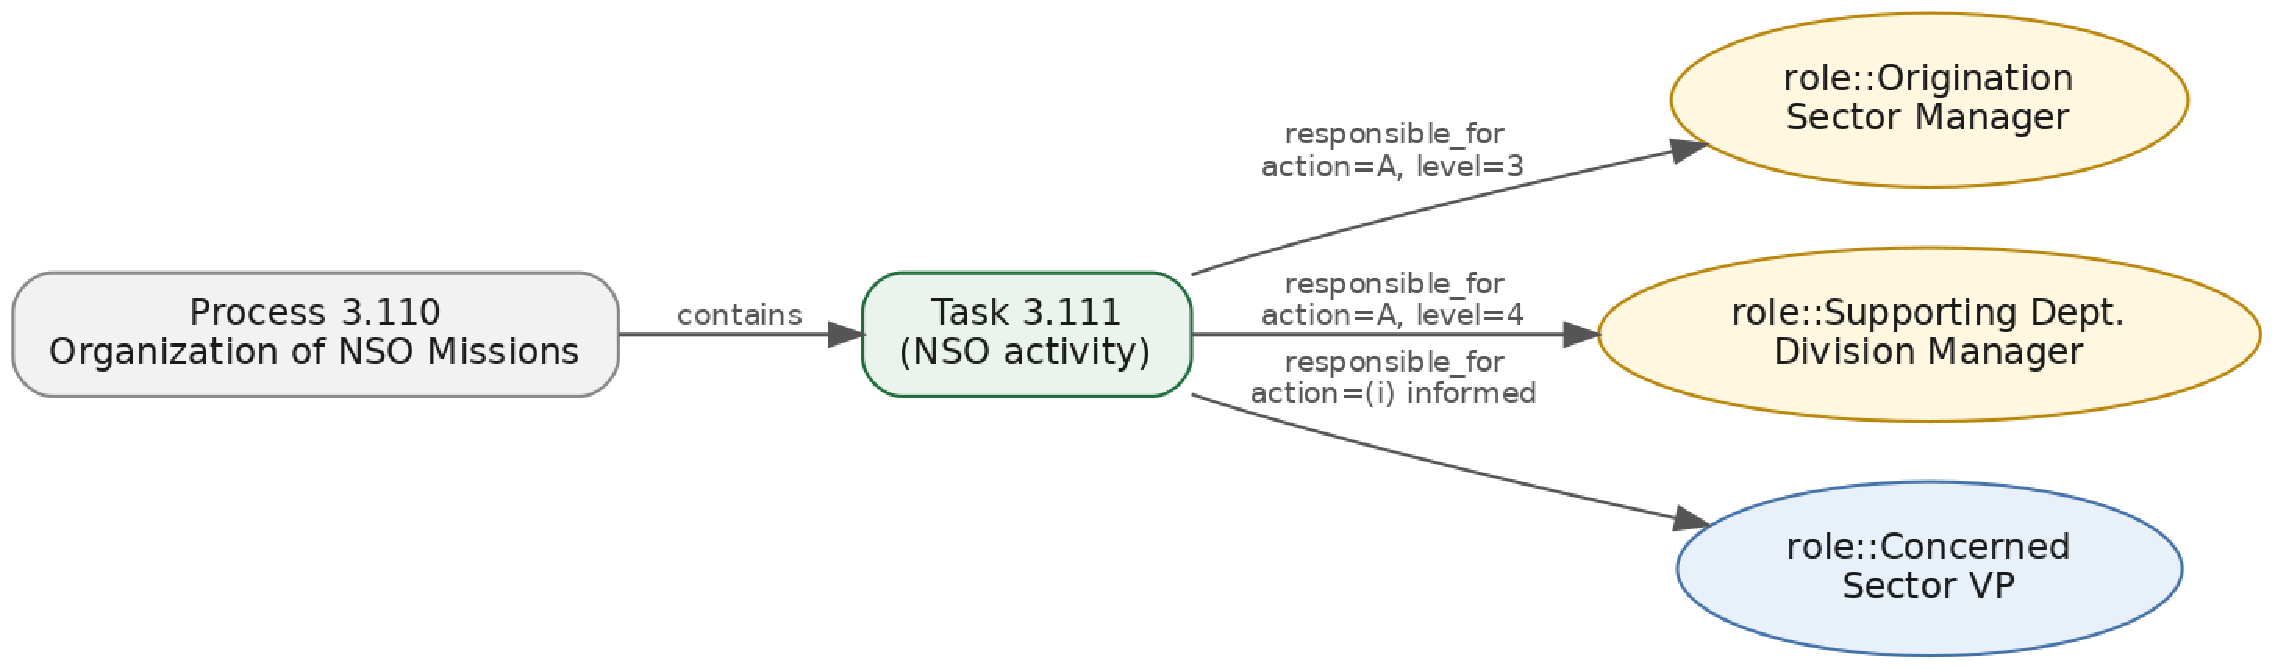
\includegraphics[width=0.94\textwidth,height=0.88\textheight,keepaspectratio]{figures/fig3_graph.pdf}
\caption{Excerpt of the knowledge graph around activity 3.111, showing the containment edge from its parent process and the responsibility edges connecting it to its approving and informed roles.}
\label{fig:graph}
\end{figure}

\subsection{Graph Statistics}

The assembled graph holds 459 nodes and 2,108 edges. The node count is the sum of the 327 activities and the 131 roles, plus one aggregate node. The edge count is dominated by responsibility edges, with containment edges accounting for the hierarchy and a small number of reference edges added from cross-references.

\section{Pipeline Evaluation}

A pipeline that runs is not the same as one that can be trusted. Both the extraction step's
runtime behaviour and the data-quality checks applied to its output are covered below, since
output is not allowed anywhere near a user's question until it passes them.

\subsection{Execution and Caching}

It takes around fifteen to twenty seconds to reconstruct the document from the PDF. This time frame is fine in an offline scenario but unacceptable when requested; hence, the node set that is being built is written into a cache file and later read during application initialization. The service running will never access the PDF while working.

The above arrangement deviates from the original one; the explanation for this change is provided in Chapter 5. The original implementation started by parsing the document when the application was initialized and was halted by the hosting system because of memory limit issues. Caching solved this problem, and in addition, this change prevented a more hidden problem, which is relying on the runtime environment to parse the document.

\subsection{Data Quality Outcomes}

The role that is unresolved For the subset that was processed, there are missing titles in record 2.516 and record 2.522, and one record (2.222.1) remains partially corrupted. Rather than being accepted and unstated, all three are known and documented. There was a candidate fix for the last case that was applied and tested but found to be not a fix for the target case but a regression in another case, so it was reverted. This was thought to be a better result than to leave a documented defect where a change could be made to make the overall extraction more desirable.

The second restriction is further discussed in the general conclusion and is due to the footnotes. Footnote reference numbers are captured and remain unchanged in respect of responsibilities and the bottom of the page text will not yet be parsed so that the system can say that a qualification is applicable if the text says so. During testing two similar extraction defects were found: a column header was confused as a role name, while two adjacent footnote digits were joined into one number in the same records. The planned remediation is also documented along with these two in Chapter~5.

But only three chapters have been exercised against the pipeline. The remainder of the entire document has the same table conventions as far as the present document is concerned, but for purposes of this document, at least, and certainly as part of a continuation of the work, such tables would be the first step in processing them.ved at a rate of 0.56 percent is the key quality measure of the pipeline and deserves careful consideration. This rate is the ratio of the number of responsibility items extracted, for which there was no matching column header. This is not related to checking whether the right code has been extracted for each cell, and this is an assessment that can only be done manually because of the lack of a ground truth dataset. This issue was examined by sampling and comparing particular activities against the printed page.

\subsection{Observed Limitations}

For the subset that was processed, there are missing titles in record 2.516 and record 2.522, and one record (2.222.1) remains partially corrupted. Rather than being accepted and unstated, all three are known and documented. There was a candidate fix for the last case, that was applied, tested, but found to be not a fix for the target case but a regression in another case so it was reverted. This was thought to be a better result than to leave a documented defect where a change could be made to make the overall extraction more desirable.

The second restriction is further discussed in the general conclusion and is due to the footnotes. Footnote reference numbers are captured, and remain unchanged in respect of responsibilities and the bottom of the page text will not yet be parsed so that the system can say that a qualification is applicable if the text says so. During testing two similar extraction defects were found: a column header was confused as a role name while two adjacent footnote digits were joined into one number in the same records. The planned remediation is also documented along with these two in Chapter~5.

But only three chapters have been exercised against the pipeline. The remainder of the entire document has the same table conventions as far as the present document is concerned but for purposes of this document, at least, and certainly as part of a continuation of the work, such tables would be the first step in processing them.

\section*{Conclusion}
\addcontentsline{toc}{section}{Conclusion}
The pipeline transforms a low-level document that is only graphically organized into 327 records that are validated and have 1776 responsibility entries, with less than 1 percent of those entries unassigned, and it converts the output into a graph of 459 nodes and 2108 edges that can answer questions about relations by traversal. Each stage is deterministic and inspectable, which enabled the defects as described in Chapter~2 to be detected, corrected, and staved off. The next chapter adds the agent that queries this graph.
\chapter{Retrieval, Grounded Generation and Agent Design}
\label{ch:agent}
\minitoc

\section*{Introduction}
\addcontentsline{toc}{section}{Introduction}
The facts are stored in the knowledge graph. This chapter explains the layer that converts a typed and/or spoken query into an answer from it. These are three problems that need to be solved in order: figuring out what the user is talking about, figuring out what he wants to know about it, and saying it back to him in a way that doesn't go against the grain of the situation.

The third is the place the majority of design work went, which sets this system apart from the typical retrieval-augmented assistant\citep{lewis2020rag}. This language model is not relied on to make any decisions. It is fed facts it has already retrieved and can only be asked to restate them; no results are presented until it confirms what it has said with the facts.

\section{Retrieval Methodology}

Resolving what a question is about comes before anything can be said about it, and the
system takes two different routes depending on how the question is phrased: a fast,
unambiguous path for a question naming an identifier directly, and a ranked free-text path
for everything else. Both routes are described below, along with the numeric gates that
decide what a free-text score is allowed to become.

\subsection{Identifier Fast Path}

If a question has something in it that looks like an activity identifier, it first attempts a direct look-up. Identifiers are unique, so there is no ambiguity and a match is precise. This route is the low cost route, and it's the one that is used by those users who already know what they're looking for.

If an identifier is not found in the node set, it is considered as a different result and not as a failure. This distinction is not as insignificant as it may seem. Previously, an unrecognised identifier would be matched with free text search over the entire question, including the bogus identifier itself. The other words of the question (such as ``task'', ``who'', and ``approves'') have enough common vocabulary with real activity titles to score positive, but would have been confused with the actual activity a user was asking about. The behaviour was not an edge case situation, but a natural case.

\subsection{Identifier Grammar and the Invalid-Identifier Branch}
\label{sec:idgrammar}

An identifier is recognised by the pattern
\texttt{\textbackslash d+(\textbackslash.\textbackslash d+)\{1,3\}(\textbackslash.[a-z])?},
which admits between two and four dotted numeric components and an optional trailing letter.
It therefore matches \texttt{2.126}, \texttt{1.117.2}, \texttt{2.432.4.a} and rejects a bare
integer, so an ordinary monetary figure in a question is not mistaken for an activity
reference.

Recognition and existence are separate tests, and the separation produces three outcomes
rather than two. A matched string that is a key in the node set resolves immediately at
confidence $1.0$. A matched string that is not a key routes to a distinct
\texttt{invalid\_id} outcome. A query containing no identifier-shaped substring at all falls
through to the free-text path.

The middle outcome exists because merging it into free-text search produces a specific
failure. A question such as ``who approves 9.999.999'' still contains the words
\emph{who} and \emph{approves}, and those words alone are sufficient to score against some
unrelated real activity. The system would then answer confidently about an activity the user
never named. Routing the case separately means the response states that the identifier does
not exist.

Suggestions accompanying that refusal are computed by longest shared dotted prefix. For an
invalid identifier $x$, every indexed node whose leading component equals that of $x$ is
ranked by

\[
\operatorname{depth}(x, n) \;=\; \max \{\, j : x_{1..j} = n_{1..j} \,\},
\]

the number of leading dotted components the two share, and the three highest are returned.
If the leading component itself matches no node, the identifier is stripped from the query
and the remaining words are put through the text index instead, so a malformed reference
accompanied by a usable description still yields candidates.

\begin{figure}[htbp]
\centering
% ---------------------------------------------------------------
% PLACEHOLDER — replace with a flow diagram of the resolution path:
%   query -> identifier regex match?
%        yes -> exists in node set? -> resolve (score 1.0)
%                                   -> invalid_id + prefix suggestions
%        no  -> typo correction -> TF-IDF -> threshold gate
%                -> answer / clarify / refuse
% Suggested filename: figures/fig5_resolution_flow.png
% ---------------------------------------------------------------
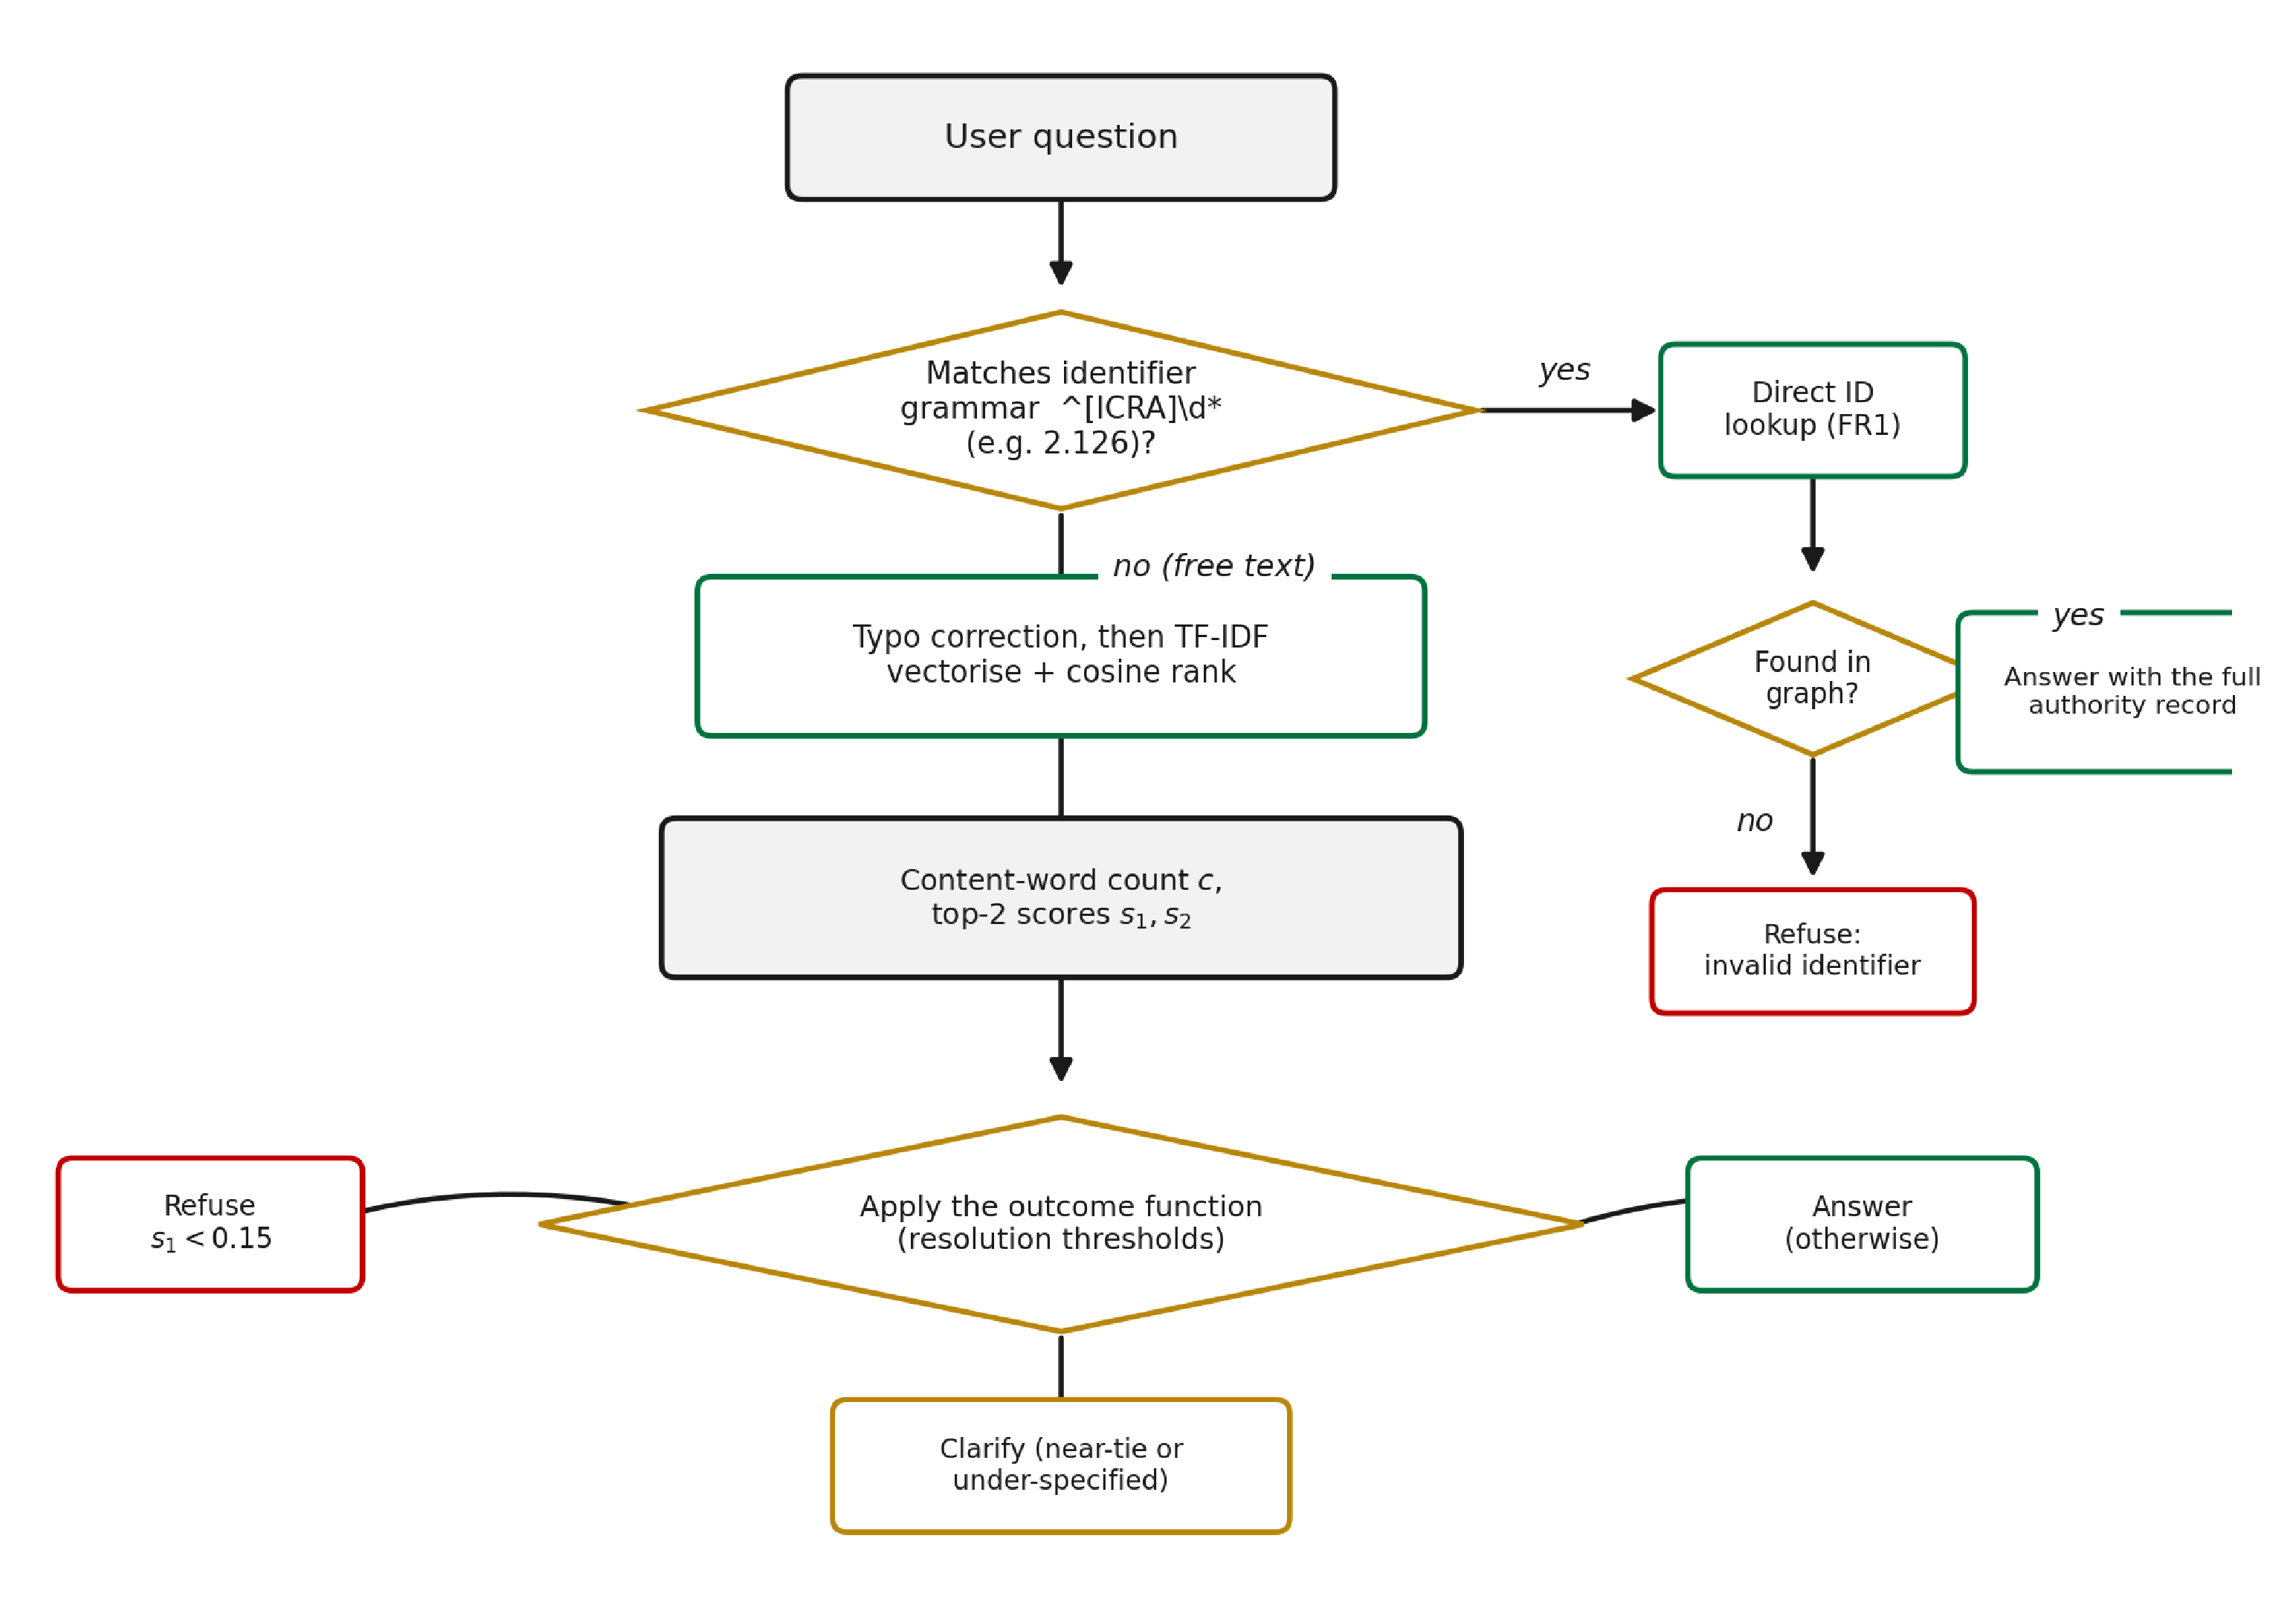
\includegraphics[width=0.9\textwidth]{figures/fig5_resolution_flow.pdf}
\caption{Resolution decision flow, from raw query to one of four outcomes: identifier
resolution, invalid-identifier refusal, clarification, or a scored free-text match.}
\label{fig:resolutionflow}
\end{figure}

Figure~\ref{fig:resolutionflow} shows the complete path, including the threshold gate
described in Section~\ref{sec:confidence}.

\subsection{Free-Text Resolution}

If the question mentions an activity but not any specific activity, lexical similarity is used to resolve the question. Each activity is represented in a vector using TF-IDF\citep{salton1988,manning2008ir} and a comparison is performed to the question by cosine similarity, returning the vector with the highest score and its value.

Tasks and child tasks, as well as process-level titles, are included in the index. Initially they were excluded because they didn't ask about activities, they asked about grouping organisations. The user was asking about the organisation of missions in the non-sovereign chapter, and so he was seeking to match nothing useful, since the only node with a title that had that phrasing was a process, and processes were not indexed.

\subsection{Index Construction}
\label{sec:indexconstruction}

The free-text path is served by a TF-IDF index\citep{salton1988,manning2008ir} fitted once at
startup and held in memory for the lifetime of the process. Table~\ref{tab:indexparams} gives
its configuration.

\begin{longtable}{|p{0.26\textwidth}|p{0.22\textwidth}|p{0.42\textwidth}|}
\caption{Configuration of the TF-IDF retrieval index.}\label{tab:indexparams}\\
\hline
\rowcolor{myblue}\textcolor{white}{\textbf{Parameter}} & \textcolor{white}{\textbf{Value}} & \textcolor{white}{\textbf{Effect}} \\
\hline
\endfirsthead
\hline
\rowcolor{myblue}\textcolor{white}{\textbf{Parameter}} & \textcolor{white}{\textbf{Value}} & \textcolor{white}{\textbf{Effect}} \\
\hline
\endhead
Corpus unit & Activity title & One document per indexed node; the title is the only field vectorised. \\ \hline
Indexed node types & \texttt{process}, \texttt{task}, \texttt{child\_task}, \texttt{threshold\_variant} & Chapter nodes are excluded, since chapter titles are empty in the extracted set. \\ \hline
Empty-title filter & applied & A node whose title is blank after normalisation contributes no row. \\ \hline
\texttt{stop\_words} & \texttt{"english"} & Removes closed-class English words before weighting, so shared function words do not raise a score. \\ \hline
\texttt{ngram\_range} & $(1,2)$ & Indexes unigrams and bigrams. A two-word phrase such as ``mission programme'' contributes a term of its own in addition to its parts. \\ \hline
Similarity & Cosine & Scores lie in $[0,1]$; $0$ means the query and title share no weighted term. \\ \hline
Candidates returned & $k = 5$ & The ranked list the resolution layer receives. Zero-scoring rows are discarded before return. \\ \hline
Mutability & Read-only after fit & The matrix is never refitted at runtime, so an identical query returns an identical ranking for the life of the deployment. \\ \hline
\end{longtable}

Including bigrams matters for this corpus because DAM titles are short noun phrases in which
word order carries meaning. ``Report to the Board'' and ``Board report'' share every unigram
and no bigram, and a unigram-only index scores them identically.

Given a query $q$ and the set of indexed titles $D$, the resolved candidate set is

\[
R(q) \;=\; \operatorname*{arg\,top-}_{d \in D}{}^{k}\;
\frac{\mathbf{v}(q)\cdot\mathbf{v}(d)}{\lVert \mathbf{v}(q)\rVert\,\lVert \mathbf{v}(d)\rVert},
\qquad k = 5,
\]

where $\mathbf{v}(\cdot)$ is the TF-IDF transform described above. The score is lexical
overlap. A score of $0$ states that the query shares no weighted term with the title, which
is not the same claim as the activity being unrelated to the question.

\subsection{Why Lexical Retrieval Rather Than Embeddings}

The more popular solution is semantic retrieval using learned embeddings – this is the one that would apply to a large and diverse body of ordinary language text. The volume of this corpus is not large and it is not representative. It's a handful of hundred short papers that have been expressed in a specific institutional jargon, such that the words the user will type are the ones most likely used by the document.\\[0.3cm]
Lexical matching is also explainable: this is a property that is important for this project. The shared terms can be carried as a score, a mismatch can be identified by analyzing the vocabulary, and the entire layer runs without downloading a model, without an inference cost, and without relying on an external service. As retrieval accuracy was the key for everything else, it was more valuable to be able to reason about why a given node was returned than to get the additional recall that an embedding model might have provided.

\subsection{Typo Tolerance}

People misspell things, particularly long institutional phrases. Rather than relying on a language model to interpret intent, the system applies a deterministic correction step: each alphabetic word in the question is compared against the vocabulary the document itself uses, and replaced with the closest match when the similarity exceeds a threshold and the word is not already an exact match.

The threshold was calibrated against a real false positive rather than chosen by intuition. Set too low, ordinary words get rewritten into document vocabulary they merely resemble, which corrupts questions that were correct to begin with. Because the step is deterministic, it behaves identically whether or not a language model provider is reachable.

\subsection{Correction Algorithm and Parameters}
\label{sec:typoparams}

Correction runs before vectorisation and operates on the query alone; the index is never
altered. Each alphabetic token is compared against the vocabulary of single words the
vectoriser already holds, so the correction target is the document's own wording rather than
a general English dictionary. A token identical to a vocabulary entry under case folding is
left alone. Otherwise the closest vocabulary entry is retrieved by Ratcliff--Obershelp
sequence matching, and the token is replaced only when that similarity reaches the threshold
in Table~\ref{tab:typoparams}. A token with no sufficiently close match is passed through
exactly as typed.

\begin{longtable}{|p{0.27\textwidth}|p{0.17\textwidth}|p{0.46\textwidth}|}
\caption{Parameters governing deterministic typo correction.}\label{tab:typoparams}\\
\hline
\rowcolor{myblue}\textcolor{white}{\textbf{Parameter}} & \textcolor{white}{\textbf{Value}} & \textcolor{white}{\textbf{Effect}} \\
\hline
\endfirsthead
\hline
\rowcolor{myblue}\textcolor{white}{\textbf{Parameter}} & \textcolor{white}{\textbf{Value}} & \textcolor{white}{\textbf{Effect}} \\
\hline
\endhead
Similarity measure & Ratcliff--Obershelp ratio & Length-normalised, in $[0,1]$. Computed against the index vocabulary, not an external dictionary. \\ \hline
Acceptance threshold & $0.88$ & A token is replaced only at or above this similarity. Below it, the token is left as typed. \\ \hline
Minimum token length & $4$ characters & Tokens of three characters or fewer are skipped entirely. \\ \hline
All-capital tokens & Skipped & A fully capitalised token is treated as an institutional acronym and never corrected. \\ \hline
Candidates considered & $1$ & Only the single closest vocabulary entry is eligible. \\ \hline
Capitalisation & Preserved & A corrected token keeps the leading case of the token it replaces. \\ \hline
Scope & Query only & The index, the stored titles, and the answer text are untouched. \\ \hline
\end{longtable}

Two of these guards address distinct failure modes. The length floor exists because
similarity is close to uninformative on very short tokens: at one to three characters a large
fraction of the vocabulary sits above any usable threshold, so short words would be rewritten
arbitrarily. The all-capitals rule exists because the DAM's role and authority vocabulary is
dense with acronyms such as \texttt{DDG}, \texttt{RDG} and \texttt{PGCL}, and fuzzy-matching
an acronym against a vocabulary of English title words can convert a correct token into an
unrelated common word.

The effect on retrieval is direct. TF-IDF has no inherent tolerance for misspelling: a
misspelled token is simply out of vocabulary and contributes nothing to the score, so a query
carrying the right words with the wrong spelling scores as though those words were absent.
Correcting before vectorisation restores the contribution rather than compensating for its
loss afterwards.

\section{Evaluation Protocol and Confidence Semantics}

There is no held-out test set here, because there is no labelled corpus to hold out. Correctness is established instead by comparison against the source document, and every resolution carries a method label and a confidence value so that the basis of an answer is visible to the user rather than implied.

Every answer carries the method by which its activity was resolved, and that label is shown to the user rather than kept internal. Table~\ref{tab:methods} states what each method means and how much weight an answer resolved that way should be given.

\begin{longtable}{|p{0.48\textwidth}|p{0.46\textwidth}|}
\caption{Resolution methods and their interpretation.}\label{tab:methods}\\
\hline
\rowcolor{myblue}\textcolor{white}{\textbf{Method}} & \textcolor{white}{\textbf{Interpretation}} \\
\hline
\endfirsthead
\hline
\rowcolor{myblue}\textcolor{white}{\textbf{Method}} & \textcolor{white}{\textbf{Interpretation}} \\
\hline
\endhead
\texttt{id} & Exact identifier match. No ambiguity. \\ \hline
\texttt{text\_search} & Resolved from the activity's name. The score is shown, and low scores are flagged in the interface. \\ \hline
\texttt{invalid\_id} & An identifier was recognised in the question but does not exist in the document. \\ \hline
\texttt{needs\_clarification} & The question is too vague to resolve to a single activity. \\ \hline
\texttt{out\_of\_scope} & The question is not about the subject matter of the document. \\ \hline
\texttt{glossary} & The question asked for the expansion of an abbreviation. \\ \hline
\texttt{action\_code\_legend} & The question asked what an authority code means. \\ \hline
\texttt{smalltalk} & Conversational input with no lookup component. \\ \hline
\end{longtable}


Exposing the method alongside the answer is a small decision with a large effect on trust. A user who can see that an answer came from an exact identifier match treats it differently from one resolved by name at a middling similarity score, and that difference in treatment is appropriate.

\subsection{Resolution Thresholds}
\label{sec:confidence}

A ranked candidate list is not yet an answer. Four numeric gates sit between the ranking and
the response, and together they determine whether the system answers, asks for
clarification, or refuses. Table~\ref{tab:thresholds} states them.

\begin{longtable}{|p{0.22\textwidth}|p{0.11\textwidth}|p{0.55\textwidth}|}
\caption{Thresholds governing the outcome of a free-text resolution.}\label{tab:thresholds}\\
\hline
\rowcolor{myblue}\textcolor{white}{\textbf{Gate}} & \textcolor{white}{\textbf{Value}} & \textcolor{white}{\textbf{Behaviour}} \\
\hline
\endfirsthead
\hline
\rowcolor{myblue}\textcolor{white}{\textbf{Gate}} & \textcolor{white}{\textbf{Value}} & \textcolor{white}{\textbf{Behaviour}} \\
\hline
\endhead
Answer floor & $0.15$ & A top score below this value is not answered. The query is treated as unresolved rather than matched to its nearest title. \\ \hline
Clarification ceiling & $0.60$ & Above this score a top match is accepted even when the query is under-specified. At or below it, an under-specified query is sent to clarification. \\ \hline
Separation minimum & $0.15$ & The gap between the first and second candidate. A gap narrower than this, with a top score under $0.85$, routes to clarification rather than selecting the leader. \\ \hline
Carry-over ceiling & $0.50$ & A follow-up question scoring above this resolves on its own words; at or below it, the activity carried over from the previous exchange is used instead. \\ \hline
\end{longtable}

Two of these gates encode conditions that a single score cannot express on its own.

The separation minimum addresses near-ties. A top score of $0.42$ against a runner-up of
$0.39$ indicates that two activities match the query almost equally well, and returning the
leader presents a coin toss as a resolution. The condition is therefore evaluated on the
difference rather than the level, and it is suppressed above $0.85$, where the leader is
strong enough in absolute terms that a close second does not undermine it.

The clarification ceiling is paired with a lexical test rather than applied alone. The
system counts content words in the query, defined as tokens of at least three characters
that appear in neither the English stop-word list, nor the intent vocabulary that identifies
which authority type is being asked about, nor a small set of domain-generic terms
(\texttt{task}, \texttt{activity}, \texttt{process}, \texttt{dam}, \texttt{please},
\texttt{tell}). A query contributing one or fewer content words is under-specified: in
``what about this task'' every token is either a stop word or domain-generic, so the ranking
that results is driven by nothing the user actually specified. Such a query is answered only
when the top score clears $0.60$ on its own.

The resulting outcome for a free-text query, writing $s_1$ and $s_2$ for the top two scores
and $c$ for the content-word count, is

\[
\text{outcome} =
\begin{cases}
\text{refuse}, & s_1 < 0.15,\\[2pt]
\text{clarify}, & (c \le 1 \wedge s_1 < 0.60) \;\vee\; (s_1 - s_2 < 0.15 \wedge s_1 < 0.85),\\[2pt]
\text{answer}, & \text{otherwise.}
\end{cases}
\]

\begin{figure}[htbp]
\centering
% ---------------------------------------------------------------
% PLACEHOLDER — replace with a plot of top-1 cosine score across a
% batch of test queries, with the 0.15 / 0.60 / 0.85 gates drawn as
% horizontal lines, so the reader can see where real queries land
% relative to the thresholds.
% Suggested filename: figures/fig5_score_distribution.png
% ---------------------------------------------------------------
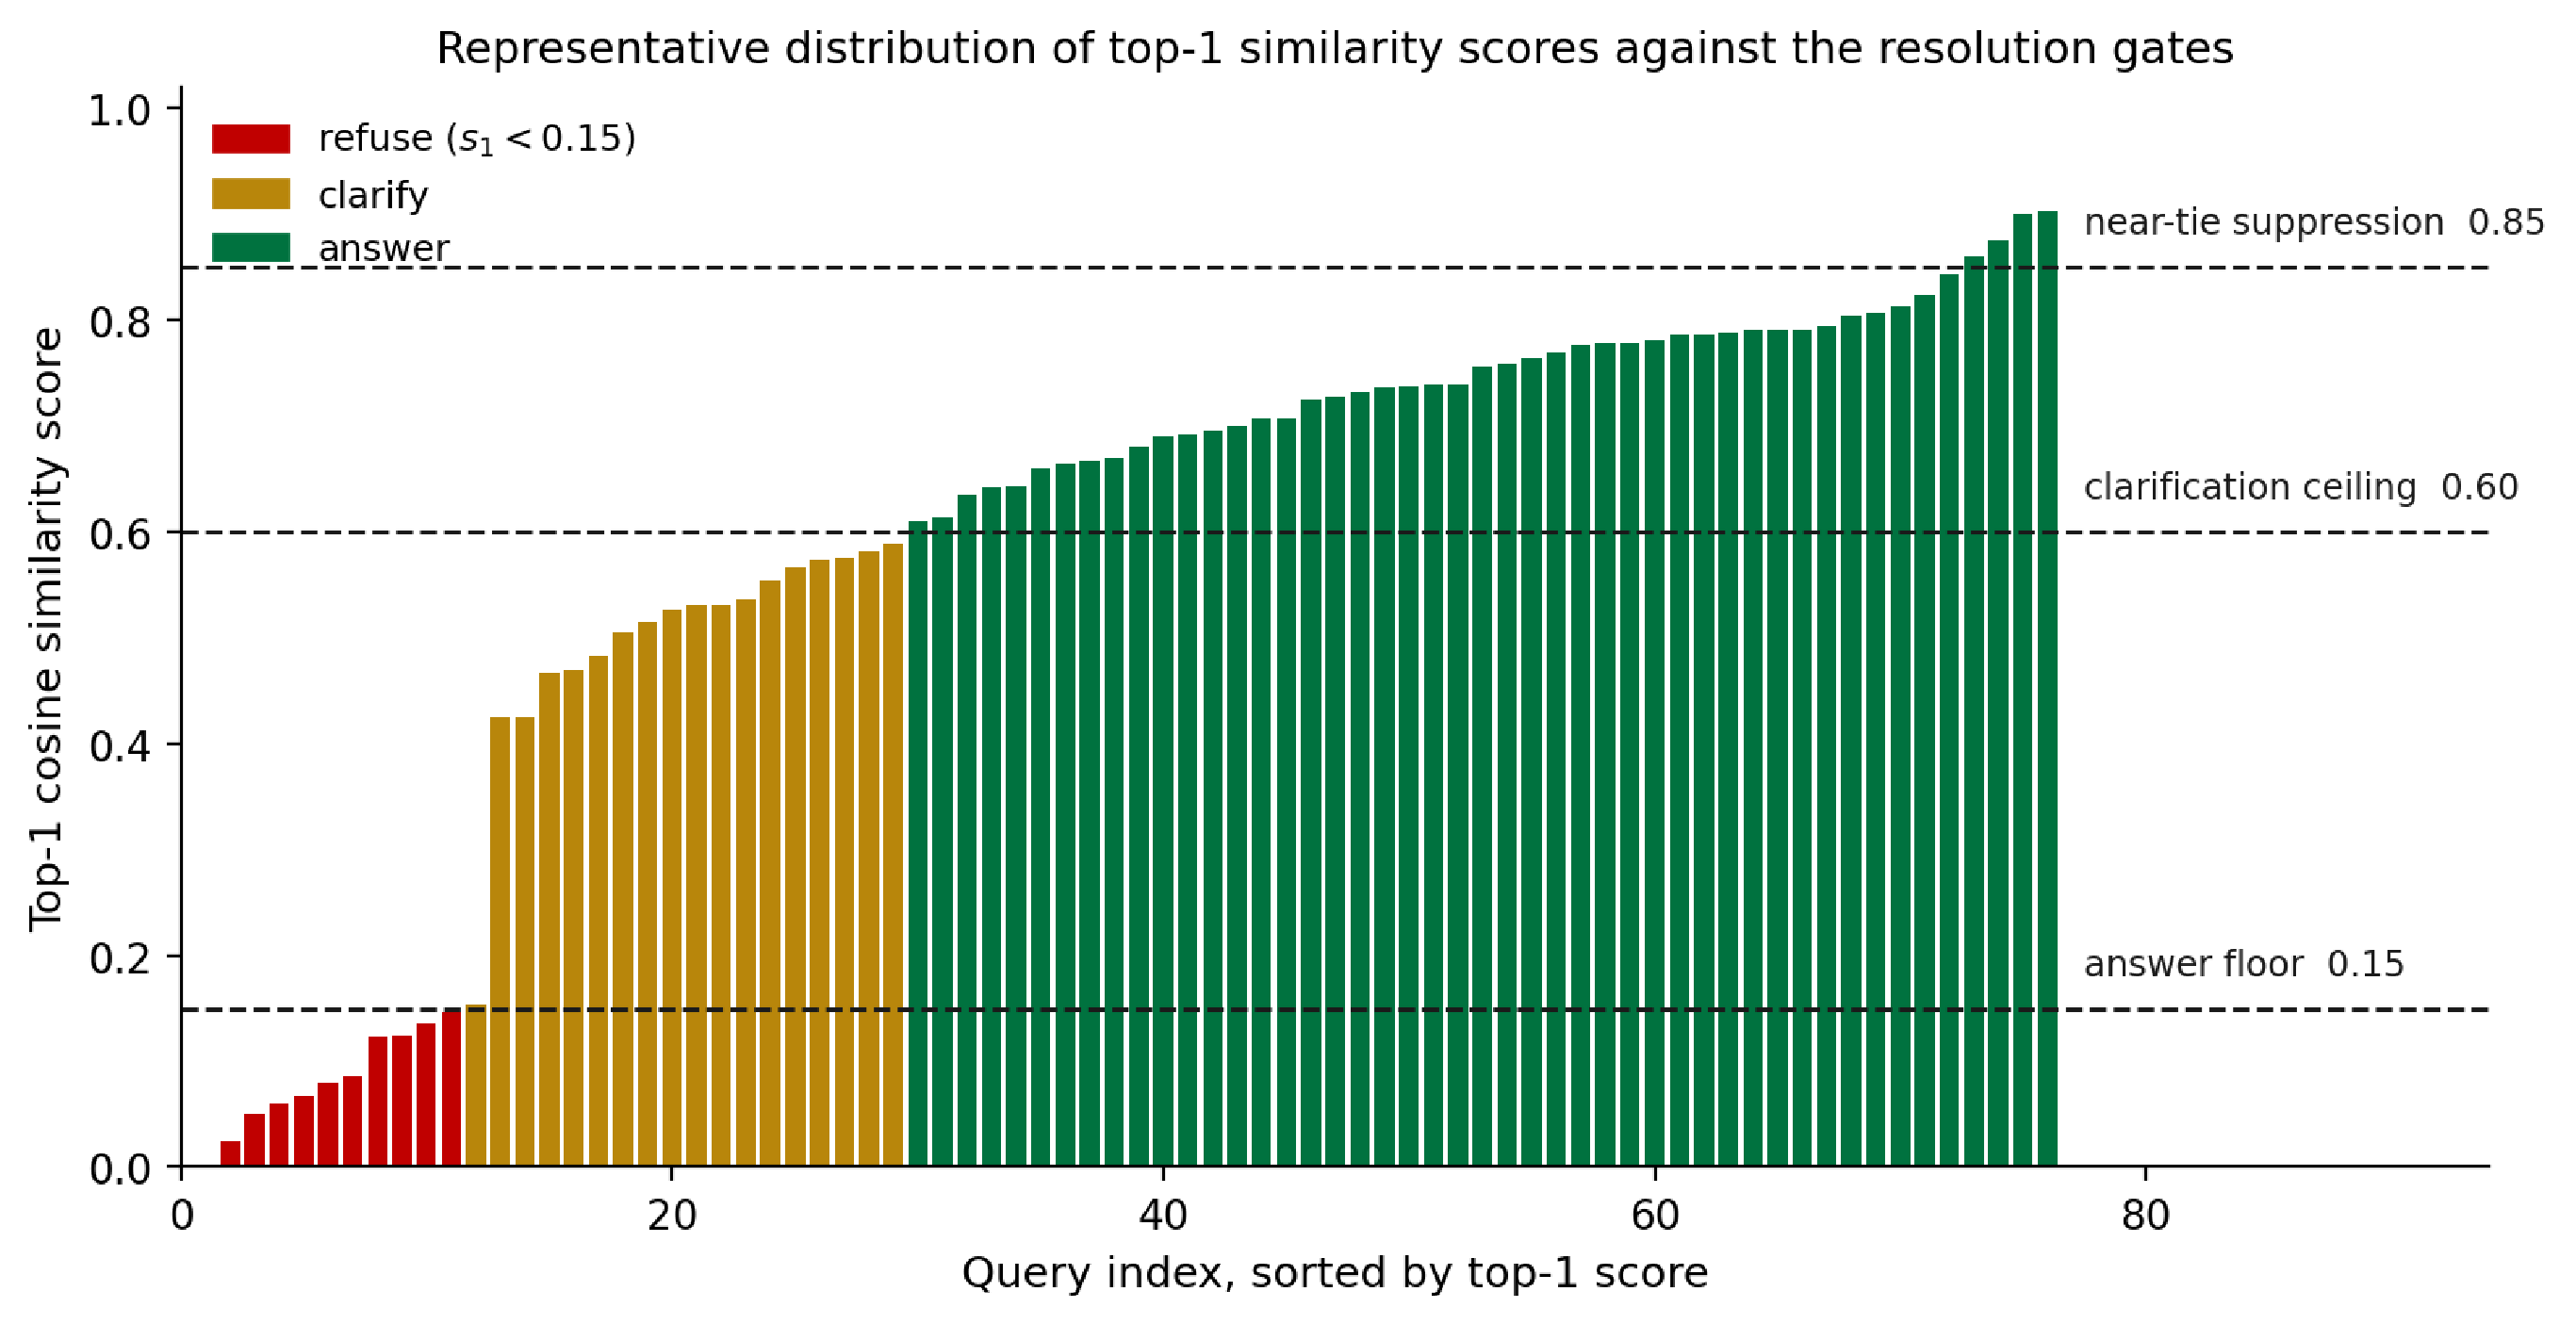
\includegraphics[width=0.9\textwidth]{figures/fig5_score_distribution.pdf}
\caption{Top-ranked similarity score across a batch of free-text queries, with the answer
floor, clarification ceiling, and near-tie suppression level marked.}
\label{fig:scoredist}
\end{figure}

Figure~\ref{fig:scoredist} places observed scores against these gates.

\section{Deterministic Answer Construction}

Once an activity has been resolved, the system still has to decide what the question was
actually asking about it, what else the document requires to be said regardless of the
question, and what to do when there is no honest answer to give.

\subsection{Intent Detection}

When the activity has been classified, the system then knows what kind of question is being asked about it. Questions are mapped to authority codes in the document, and the mapping needs to take into account how people ask these questions, with ``who signs off on this?'' meaning an approval and ``who has to check this?'' meaning check and verify.

This mapping cannot be naive when it comes to the letter C. According to Chapter~1, C1 and C2 are check and verify whereas C3 and C4 are consult, and mapping ``check'' to the letter C would be mixing up two different duties. This is why intent detection is against full codes and not their initial letter.

\subsection{Mandatory Obligation Surfacing}

Where an answer provides the response to the question, it also includes that which the document requires to be included. In the case of an action that has a check-and-verify entry in the DAM, that entry will appear even where the question pertained to the approval entry. The names of any informed individuals on record will appear.

This is because this is not an addition of contextual information. It is simply a required entry in the DAM, and it is someone new to the company asking the very specific question who will need the other three answers. This note is hidden only if it would repeat the answer provided.

\subsection{Cross-Reference Following}

Where a resolved activity has no responsibilities of its own but does carry a cross-reference, the system follows the reference and reports the target's responsibilities, stating that it has done so. This mirrors what a human reader does when a row tells them to look elsewhere, and it converts a dead end into an answer.

\subsection{Honest Refusal}

Three situations lead to a non-answer. In the case of an identifier that doesn't exist, the fact that it doesn't exist is stated, and a request is made to validate the identifier or describe what is happening. When a question is too vague to answer, the user is asked to provide additional information. When a question is off-topic, it is considered out of scope.

This is what should not happen in any of these scenarios. This is what requirement FR7 asks for and what makes positive answers valuable: a machine that knows all does not tell us anything about the reliability of its answers.

\section{Auxiliary Query Types}

But not all queries are authority queries. There are three more query types that get answers directly.

Glossary queries ask for the definition of an abbreviation and are answered using the abbreviations found in the document along with a small list of aliases for the acronyms found in role descriptions and not explicitly expanded. If the answer comes from the list of aliases, then the source of the definition is reported.

Authority-code queries ask for the definition of a code and are answered from the legend of the transcription. Authority codes detection is conservative on naked codes to avoid collision of 'I' with the pronoun. A naked code becomes a real mention only if it appears in the same sentence with some other code or is unambiguously used, like the parenthesized informed status marker or an alphanumeric combination not forming an English word.

Input queries are matched to anchored patterns and answered directly, bypassing the lookup pipeline. Patterns match anchored to the whole query string to avoid matching of 'hi' in the phrase 'history of the DAM'.

\section{Hybrid Language Model Layer}

Answer phrasing is delegated to a language model through a provider interface with two implementations and four operating modes.

\begin{longtable}{|p{0.16\textwidth}|p{0.30\textwidth}|p{0.44\textwidth}|}
\caption{Language model providers and operating modes.}\label{tab:llm}\\
\hline
\rowcolor{myblue}\textcolor{white}{\textbf{Mode}} & \textcolor{white}{\textbf{Provider}} & \textcolor{white}{\textbf{Behaviour}} \\
\hline
\endfirsthead
\hline
\rowcolor{myblue}\textcolor{white}{\textbf{Mode}} & \textcolor{white}{\textbf{Provider}} & \textcolor{white}{\textbf{Behaviour}} \\
\hline
\endhead
Auto & Cloud, falling back to local, then template & Default. Uses whichever provider is available, and the deterministic template if neither is. \\ \hline
Cloud & Groq\citep{groq} & Hosted inference. Fast, requires an API key and network access. \\ \hline
Local & Ollama\citep{ollama} & Runs on the same machine or in a companion container. No external dependency. \\ \hline
Off & None & Template answers only. Every lookup capability remains available. \\ \hline
\end{longtable}

It has been intentionally designed such that the agent and the providers interface is very small, and this has served to be of great benefit in the course of the project where a hosted model was deprecated by the provider and started throwing errors in the deployment environment. The solution was a mere modification of a constant behind the interface, without any impact on the agent and its tests.

\subsection{Model Configuration}
\label{sec:modelconfig}

Table~\ref{tab:models} records the models each mode resolves to and the task each performs.
Every identifier is read from configuration rather than compiled in, so a deprecated model
is replaced without a code change.

\begin{longtable}{|p{0.20\textwidth}|p{0.30\textwidth}|p{0.38\textwidth}|}
\caption{Models used by task, with the mode that selects each.}\label{tab:models}\\
\hline
\rowcolor{myblue}\textcolor{white}{\textbf{Task}} & \textcolor{white}{\textbf{Model}} & \textcolor{white}{\textbf{Notes}} \\
\hline
\endfirsthead
\hline
\rowcolor{myblue}\textcolor{white}{\textbf{Task}} & \textcolor{white}{\textbf{Model}} & \textcolor{white}{\textbf{Notes}} \\
\hline
\endhead
Answer phrasing, hosted & \texttt{openai/gpt-oss-120b} & Default for the hosted mode. Reached over an OpenAI-compatible chat completions interface. \\ \hline
Answer phrasing, local & \texttt{llama3.1} & Default for the local mode, served on \texttt{localhost:11434}. Selected when no hosted credential is present and the local service answers. \\ \hline
Transcription & \texttt{whisper-large-v3-turbo} & Converts a dictated audio clip to text. Hosted only; the local mode has no transcription path. \\ \hline
Image understanding & \texttt{qwen/qwen3.8-27b} & Used for image attachments. Requested through the same endpoint with an image content part carrying a base64 data URL. \\ \hline
Translation and tone & As answer phrasing & Both reuse whichever provider the active mode resolved to; neither has a model of its own. \\ \hline
\end{longtable}

Vision support is a property of the provider rather than of the mode. The provider interface
exposes a capability flag that is false by default and true only for the hosted provider, and
the attachment path tests that flag before constructing a request. An image sent while the
local mode is active is refused with a statement of the limitation rather than dispatched to
a model that would ignore it.

\subsection{Language Detection}
\label{sec:langdetect}

Translation is expensive relative to retrieval, so a deterministic pre-filter decides whether
the translation path runs at all. The filter uses three tests and returns true on the first
that matches: presence of any character in the Arabic block \texttt{U+0600}--\texttt{U+06FF};
presence of an accented Latin character from the set
\texttt{àâäéèêëïîôöùûüçñãõ}; or a whole-word match against per-language function-word lists
holding French, Spanish and Portuguese closed-class terms.

A single function-word hit is sufficient. The threshold is set there because a realistic
short question contains very few of them once domain vocabulary is excluded: the French
phrasing of ``who approves 3.111'' contributes exactly one, namely \emph{qui}. Requiring two
hits fails on that query.

Setting the bar that low is only safe because of what a false positive costs. A query wrongly
flagged as non-English is sent through translation, and the model reports the language as
English and returns the text unchanged, so the cost is one additional round trip and never an
altered answer. The word lists were also screened against ordinary English DAM vocabulary,
and ambiguous single-letter entries were removed for the same reason.

Retrieval itself is never multilingual. A non-English question is translated into English
before it reaches the index, and the answer is translated back afterwards, so the index, the
correction vocabulary, and the thresholds in Table~\ref{tab:thresholds} operate on English in
every case and behave identically regardless of the language the user typed.

\section{Grounded Generation and the Verification Check}

The facts are settled by this point; what remains is turning them into readable prose
without letting the model that does the wording quietly change what was said.

\subsection{Contract Given to the Model}

This model has no access to the knowledge graph and does not make decisions about what to retrieve. It gets a question, some set of previously retrieved facts, and a system prompt asking it to express these facts naturally without fabricating anything, omitting anything, and using any formatting. In case when the answer needs to be formulated in another language, there is an additional rule for the model that instructs it to translate the sentence without changing role names, identifiers, and footnotes.

Figure~\ref{fig:grounding} traces the complete flow, and the position of the verification step in it is the point of the diagram: the model sits inside the loop, not at its end, and nothing it produces reaches the user without being checked back against the facts it was given.

\begin{figure}[htbp]
\centering
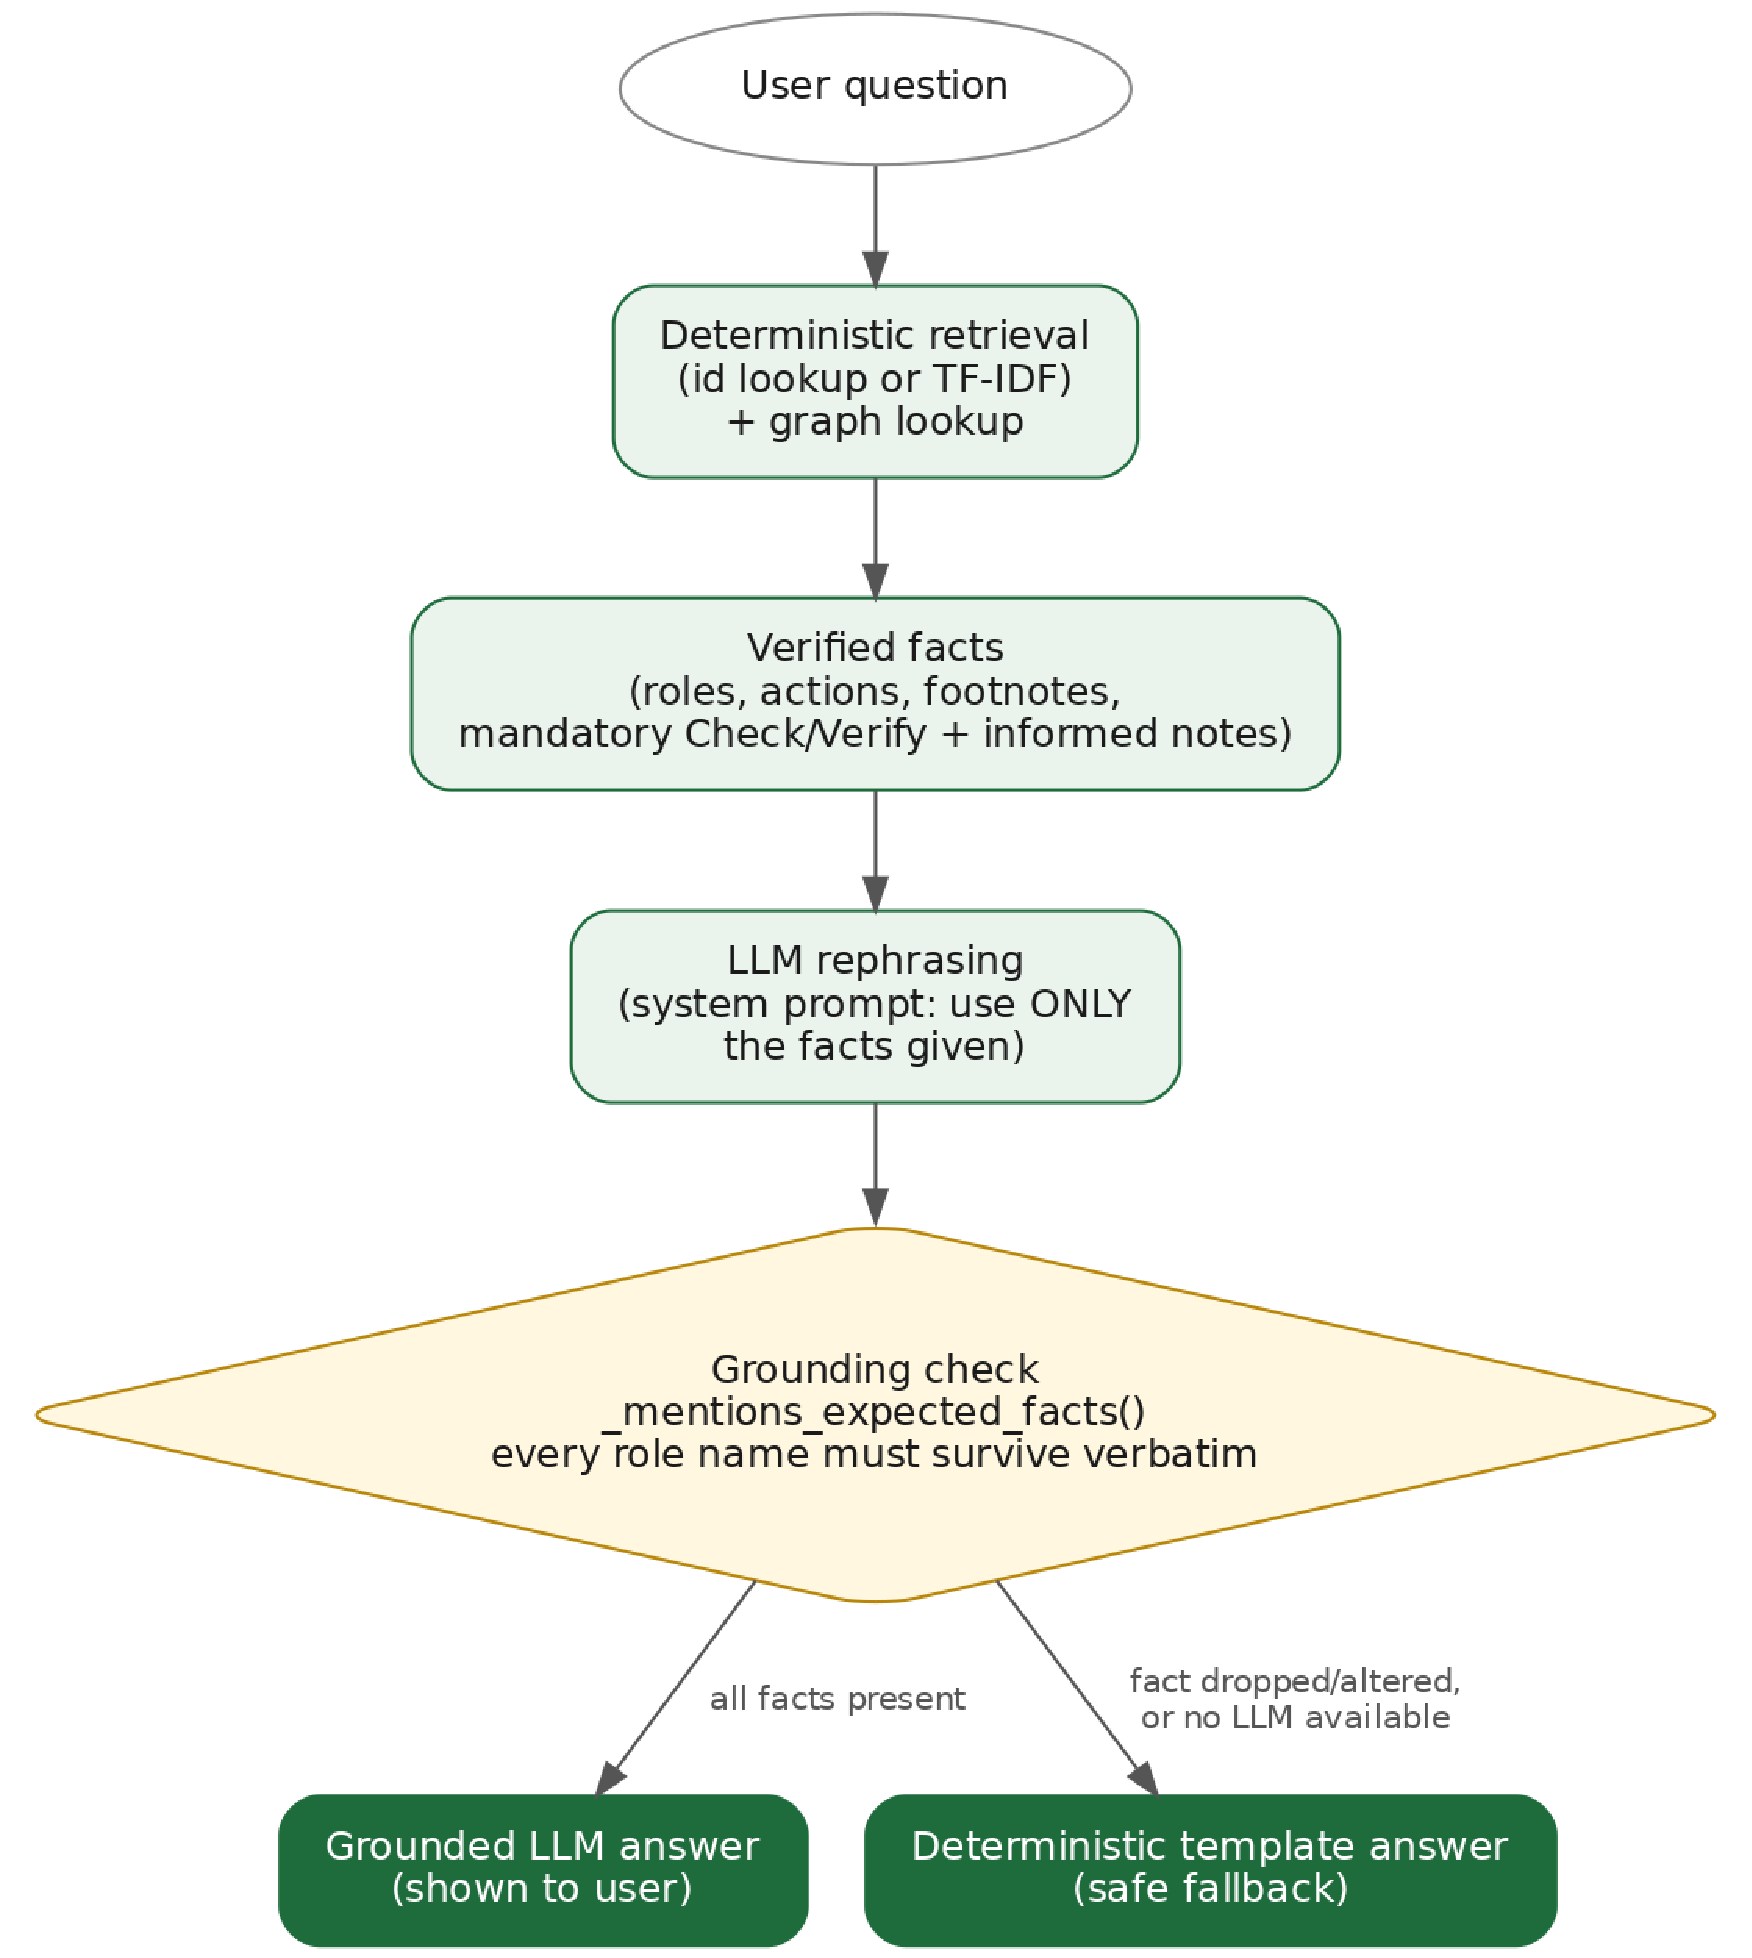
\includegraphics[width=0.94\textwidth,height=0.88\textheight,keepaspectratio]{figures/fig4_grounding.pdf}
\caption{Grounded generation flow. The model may only rephrase facts that have already been verified, and any rephrasing that drops or alters a fact is discarded in favour of the deterministic template answer.}
\label{fig:grounding}
\end{figure}

\subsection{Verification Step}
\label{sec:verification}

The instruction is a prompt, but not a guarantee. The verification converts the instruction into a property of the system.

Before the answer is generated, it is verified whether any role mentioned in the list of facts that back up the answer is found in the generated answer. In case of the absence of any of them, the generated answer is dropped, and a deterministic template answer is provided instead. The verification process relies on the containment test and not on the similarity test. Therefore, the paraphrasing of a role would not pass verification. The instruction that renamed, combined two roles into one or omitted the third role out of four informed people failed to satisfy the verification criterion regardless of fluency.

For both sides of comparison normalization of whitespace and case was applied. The reason for this tolerance was the fact that the previous version of verification used to fail some otherwise correct answers owing to mere formatting differences. The adjustment made the process less sensitive to formatting without reducing the correctness of verification, as all the same words in the same order should be present anyway.

\subsection{Answer Length and the Fallback Rate}

At first, the verification process happened more often than expected. The reason for that turned out to be a conflict between two instructions rather than the lack of reliability of the model. The instruction included in the system prompt dictated the answer containing from one to three sentences. It is impossible to articulate all duties of some activities in three sentences; hence, the model did not include some facts in accordance with the brevity instruction, and the verification was right.

The correction involved loosening the brevity condition rather than the accuracy condition. In case the number of facts backing up an answer exceeded a certain threshold, the brevity instruction was replaced by another instructing to use as many sentences as needed to cover the facts, while other constraints should stay in effect.

\section{Conversational Capabilities}

A single-turn question-answer exchange covers most of what earlier sections describe, but a
conversation is rarely that tidy in practice. The capabilities layered on top of single-turn
resolution include carrying the subject across a follow-up, adapting tone, handling
multilingual phrasing, and working from a worked example rather than a bare identifier.

\subsection{Context Carry-Over}

A user who has just asked about an activity and then asks ``and who has to be informed?''
expects the second question to be understood against the first. The client passes the
identifier resolved by the previous exchange back to the server as
\texttt{previous\_node\_id} on each subsequent request, and where a follow-up contains no
resolvable subject of its own, the retrieval layer answers it against that identifier
rather than returning a failure. The interface then states explicitly that the subject was
carried over, so that a user is never left to infer which activity an answer refers to.

Carry-over is state held by the client rather than by the server. The server remains
stateless with respect to conversational context: it is told the previous identifier on
each call instead of remembering it, which keeps a conversation reproducible from its
transcript alone and avoids any session affinity in deployment.

The mechanism required an explicit suppression rule. Carry-over was initially applied
whenever a question failed to resolve a subject, which silently captured question types
that have nothing to do with the previous activity. Asking what an authority code means
while an activity was in context produced an answer about that activity rather than about
the code, because the code question resolved no subject of its own and was therefore
treated as a follow-up. Auxiliary query types, glossary lookups, authority-code
explanations and small talk, are now classified before carry-over is considered, and are
excluded from it.

\subsection{Tone Adaptation}

Questions are classified as neutral, frustrated, or confused, and a short empathetic
opener is prepended where the tone is not neutral. The classification is gated behind a
deterministic pre-filter: a lexical check for markers of frustration or confusion decides
whether a model call is worth making at all, so a neutral question, which is the
overwhelming majority of traffic, incurs no additional latency or cost. Tone is assessed
against the text the user actually typed rather than against any internally translated
version of it, since translation normalises register and would erase precisely the signal
being measured.

Tone affects only the opener. It cannot alter the facts that follow it, which are
assembled before tone is ever considered.

\subsection{Multilingual Questions}

Questions in French, Spanish, Portuguese, or Arabic are detected, translated into English
for retrieval, and answered in the language in which they were asked. Detection uses a
deterministic pre-filter over character ranges and function-word lists rather than a model
call, so an English question, again the common case, is never charged for a capability it
does not use.

Retrieval itself remains English-only and entirely unchanged. This is deliberate: the
index, the typo-correction dictionary and the identifier grammar are all built from the
document's own English vocabulary, and translating the question before retrieval rather
than localising the index means that the retrieval behaviour tested in this chapter is
exactly the behaviour a non-English user receives. Two distinct language concerns are
kept separate in the implementation, the language a question must be translated
\emph{from} for retrieval, and the language the answer is phrased \emph{in}, so that an
English question can be answered in French when the interface language has been set
explicitly.

The verification check described in Section~\ref{sec:verification} is not translated. It
continues to search for the literal English role names inside the generated answer
whatever language the surrounding sentence is written in. A French answer that has dropped
a role therefore fails exactly as an English one would, and the guarantee does not weaken
as language support widens.

\section{Worked Examples}

The following exchanges were run against the delivered build and are reproduced as the
system produced them.

Asking \textit{``who approves 2.126''} resolves by identifier with confidence 1.0 to the
quarterly mission programme activity, and names the Regional Director General and the
Director of the Nigeria office as approvers, with the abbreviation expanded inline. The
answer also states that the task must be checked and verified by the Sector Manager and
the Supporting Department Division Manager, and that the concerned Sector Vice-President,
the Regional Vice-President, and the Task Manager or Project Team must be informed. None
of that was asked for. All of it is mandatory, and surfacing it is the behaviour required
by FR4.

Asking \textit{``who needs to be informed for quarterly mission program''} resolves the
same activity from its name alone, through the lexical path rather than the identifier
path, with the answer now centred on the informed parties.

Asking \textit{``who aproves the qaurterly mision program''}, with three deliberate
misspellings, resolves identically. The correction is deterministic, so the behaviour is
identical with or without a model provider available.

Asking \textit{``who initiates 1.117.2''} exercises the redirect path. That activity's own
row records no responsibilities and points to another activity, so the system follows the
pointer and reports the target's responsibilities instead of dead-ending on an empty
record.

Asking \textit{``who approves of Communication with Co-Financiers of projects''} followed
by \textit{``and who are the informed parties?''} exercises carry-over: the second
question, which names no subject, stays on the activity resolved by the first.

Asking \textit{``what happens with 9.999.999''} produces a refusal, stating that the
identifier does not exist and suggesting that the user check it or describe the activity
in words. This is the behaviour the design exists to produce, and it is worth reading as a
result rather than as a limitation: the alternative, a plausible answer about a
neighbouring activity, is the failure mode this entire architecture was built to prevent.

\section*{Conclusion}
\addcontentsline{toc}{section}{Conclusion}

This chapter has described how a question becomes an answer. Resolution proceeds through
an identifier fast path and a lexical search layer, both deterministic, and answers are
constructed from records held in the knowledge graph rather than generated. A language
model participates only in how an answer reads, never in what it asserts, and a
verification step compares the generated text against the retrieved facts and discards any
rephrasing that has lost one of them.

The value of that separation is that it makes a guarantee possible. Retrieval may fail,
and when it does the system says so; but an answer that is returned cannot contain a role
or an obligation the document does not record, because no component downstream of
retrieval is permitted to introduce one. Around that core sit the behaviours that make the
system usable rather than merely correct: typo tolerance, redirect following, mandatory
obligation surfacing, context carry-over, tone adaptation, multilingual handling, and
explicit refusal.

What this chapter has not addressed is everything surrounding the agent: who is allowed to
use it, how conversations persist, how answers reach a user who is not at a keyboard, and
what the accumulated structure of the matrix itself reveals when it is examined in
aggregate. The next chapter presents the platform built to deliver those.

\chapter{Implementation Results and Delivered Platform}
\label{ch:platform}
\minitoc

\section*{Introduction}
\addcontentsline{toc}{section}{Introduction}

The preceding chapter closed with an agent that resolves a question and constructs a
verified answer. That agent is a library: it has no users, no memory, and no way of
reaching anyone who is not running Python on the same machine. This chapter presents the
platform built around it, and the order of presentation follows the order in which a
capability had to exist before the next one became possible.

The chapter opens with the architecture and the boundary that separates the immutable
knowledge base from mutable application state, since that boundary is what allowed every
subsequent feature to be added without touching the components responsible for
correctness. Access control follows, because an unauthenticated system cannot own a
conversation, and without ownership neither persistence nor sharing has any meaning. The
conversation interface and its input modes come next, then conversation persistence and
the sharing mechanism built on top of it. The dashboard is treated separately and at
length: it is the one part of the platform that reports on the matrix itself rather than
answering questions about it, and it turns out to expose properties of the document that
no page-by-page reading makes visible. The chapter closes with the REST surface, the test
suite, and deployment.

\section{Application Architecture}

Two structural decisions carry the rest of this chapter: how the client and server are
split, and how the two very different kinds of data the system holds are kept apart from
each other. Both were made early and never revisited, because later features were designed
to fit them rather than the other way round.

\subsection{Client--Server Structure}

The web client is a multi-page application rather than a single-page one. It is built with
React\citep{react_docs} and bundled by Vite\citep{vite_docs} into four independent entry
points, one each for the landing page, the sign-in page, the conversation page and the
dashboard, and the backend exposes a route for each that returns the corresponding
pre-built HTML document. The compiled JavaScript and stylesheet bundles are served from
two static mounts alongside them.

The distinction between what is written and what is served is worth making explicit, since
the two are not the same artefacts. The interface is authored as React components in JSX,
a syntax no browser can execute directly. The build step compiles that JSX into plain
JavaScript, bundles it, and emits for each entry point a minimal HTML document whose only
content is an empty mount element and a reference to the compiled bundle. What the backend
serves is therefore the compiled output, not the source: no JSX file exists in the deployed
artefact, and the interface a user sees is constructed in the browser by React once that
bundle has loaded and mounted into the empty element. Nothing is rendered or templated on the server: the
backend returns files that were produced at build time, and every dynamic element of a
page is populated by the client calling the API after it loads.

This was a deliberate choice rather than a simplification, and it trades a small amount of
navigation smoothness for two properties that matter more here. A single-page application
owns its own routing, which obliges the server to answer every unrecognised path with the
application shell so that the client-side router can interpret it; get that fallback wrong
and a hard refresh on an interior route returns a 404. With one real route per page that
failure mode does not exist, because every URL a user can reach is a URL the server
genuinely serves. The second property is that authentication boundaries fall on page
loads, where the server can act on them, rather than on client-side transitions it never
observes.

Serving the client from the same process that exposes the API keeps the deployment to a
single service and removes cross-origin configuration entirely, which matters on the free
hosting tier described later in this chapter, where a second service would be a second
cold start. The backend itself is built on FastAPI\citep{fastapi_docs}.

At startup the backend loads the cached node set, constructs the knowledge graph in
memory using networkx\citep{hagberg2008networkx}, and fits the TF-IDF index over activity
titles. All three structures are held in process memory for the lifetime of the service
and are read-only thereafter. A question is therefore answered from memory, with no
database round trip and no parsing, which is what makes the response-time requirement
achievable on a free hosting tier.

The web layer contains no domain logic. Every decision about the content of an answer is
taken inside the agent; the backend authenticates the caller, hands the question to the
agent, and serialises what comes back. This separation was maintained deliberately, and
its value is visible in the development history: each platform capability described in
this chapter was added without modifying the retrieval or generation components, so no
feature in this chapter can have altered the correctness guarantee established in
Chapter~\ref{ch:agent}.

\subsection{Two Stores, Deliberately Separated}

Two kinds of data exist in the system, and almost every design decision in this section
follows from refusing to mix them.

The knowledge base is immutable. It is a serialised artefact produced by the pipeline of
Chapter~\ref{ch:pipeline}, shipped with the application, loaded into memory at startup, and
never written to at runtime. It lives in no database at all. The consequence worth stating
is that the knowledge base cannot be corrupted by application traffic: there exists no code
path by which a user action modifies what the system believes the document says. A user can
create an account, hold a hundred conversations and share every one of them, and the answer
to ``who approves 2.126'' is bit-for-bit what it was before they arrived.

Application state is the opposite in every respect. Accounts, conversations, and sharing
grants are mutable by definition, they are written on ordinary user actions, and they must
survive a process restart. They therefore live in a relational database.

Keeping the two apart is what makes the correctness argument of Chapter~\ref{ch:agent}
survive contact with a multi-user application. If the extracted matrix lived in the same
database as the conversations, then every feature added to the platform would become a
potential vector for altering the facts, and each one would need to be argued against that
possibility. Because it does not, the argument is made once, structurally, and does not need
revisiting.

\subsection{Choosing the Persistence Layer}

The database is a managed PostgreSQL instance hosted on Neon, reached through SQLAlchemy as
an object-relational mapper. Two aspects of that choice were forced rather than preferred,
and both are worth recording because the reasoning generalises.

The first is why a hosted database at all, rather than a file alongside the application. The
application is deployed on a platform whose free tier provides no persistent disk. A
file-based database written next to the running service would therefore be destroyed on
every redeployment, and the failure would be silent: the service would restart cleanly, the
schema would be recreated empty, and every registered account would simply be gone with no
error anywhere to indicate it. That is the same class of defect as the memory failure
described in Section~\ref{sec:deployment}, an assumption about the persistence of local
state that the platform does not honour, and it was avoided in advance only because the
earlier failure had already taught the lesson.

The second aspect is the local-development fallback. Requiring a hosted database to run the
test suite would make the tests slow, network-dependent, and impossible to run offline, so
the connection string defaults to a local file-based SQLite database when no environment
variable is supplied. Production sets that variable and gets PostgreSQL. This yields a
genuine engineering problem, since the two engines do not offer the same column types, and
the way it is resolved is described next.

\subsection{Identifiers and Dialect Portability}

Every table uses a randomly generated UUID as its primary key rather than an
auto-incrementing integer. The reason is not aesthetic. Conversation identifiers appear in
URLs, and a sequential integer key would make those URLs enumerable: a user holding
conversation 41 could try 40 and 42 and learn, from the difference between a refusal and a
not-found, how many conversations exist and roughly when theirs was created. Authorisation
is still checked on every request, so enumeration would not grant access, but a random
128-bit identifier removes the information leak entirely rather than relying on the check to
contain it. Identifiers are generated in the application rather than by the database, which
also means an object's identity is known before it is persisted.

The portability problem is that PostgreSQL has a native \texttt{UUID} column type and SQLite
does not. Rather than abandoning the native type in production, or maintaining two model
definitions, the schema declares the column once with a dialect variant: the type resolves to
a native \texttt{UUID} when the engine is PostgreSQL and to a 36-character string when it is
SQLite. One model definition drives both, so the objects exercised by the 375 tests on SQLite
are the same objects that run against PostgreSQL in production, and a schema change cannot
be applied to one and forgotten in the other.

\subsection{Accounts Table}

The \texttt{users} table is where the three sign-in paths converge, and its most important
property is a column that is allowed to be empty. Table~\ref{tab:usersschema} gives its
definition.

\begin{longtable}{|p{0.22\textwidth}|p{0.16\textwidth}|p{0.52\textwidth}|}
\caption{Accounts table \texttt{users}.}\label{tab:usersschema}\\
\hline
\rowcolor{myblue}\textcolor{white}{\textbf{Column}} & \textcolor{white}{\textbf{Type}} & \textcolor{white}{\textbf{Purpose and constraints}} \\
\hline
\endfirsthead
\hline
\rowcolor{myblue}\textcolor{white}{\textbf{Column}} & \textcolor{white}{\textbf{Type}} & \textcolor{white}{\textbf{Purpose and constraints}} \\
\hline
\endhead
\texttt{id} & UUID & Primary key, generated by the application. \\ \hline
\texttt{email} & string & Unique and indexed, never null. Normalised to lower case on write so that address casing cannot create two accounts. \\ \hline
\texttt{name} & string & Display name. Nullable, since a provider may not release it. \\ \hline
\texttt{hashed\_password} & string & \textbf{Nullable.} The bcrypt digest for accounts that have a password. Null for accounts created through a federated provider. \\ \hline
\texttt{oauth\_provider} & string & Nullable. Which provider authenticated this account, where one did. \\ \hline
\texttt{oauth\_sub} & string & Nullable. The provider's own immutable subject identifier for this person. \\ \hline
\texttt{role} & enum & \texttt{analyst} or \texttt{administrator}. Never null. \\ \hline
\texttt{created\_at} & timestamp & Account creation, in UTC. \\ \hline
\multicolumn{3}{|p{0.92\textwidth}|}{\textbf{Constraint} \texttt{uq\_oauth\_identity}: the pair (\texttt{oauth\_provider}, \texttt{oauth\_sub}) is unique, so one provider identity cannot be attached to two local accounts.} \\ \hline
\end{longtable}

A single table serves all three paths, and a row is distinguished only by which columns carry
values. A password account populates \texttt{hashed\_password} and leaves the two federated
columns null. A federated account does the reverse. The schema permits both at once, which is
what allows a person who signed up with a password to later authenticate through Google and
arrive at the same account rather than a second one.

The nullable password column is a security property rather than a convenience. An account
created through Google has no password anywhere in this system, so there is no digest to
extract from a database disclosure, no credential to reuse against another service, and no
password to be phished. The login endpoint enforces the corresponding rule explicitly: it
refuses when \texttt{hashed\_password} is null, so a federated account cannot be attacked
through the password form at all. Figure~\ref{fig:dbusers} shows the table as deployed, with
the bcrypt digests visible and the federated columns null for the three accounts registered
at the time of writing.

\begin{figure}[htbp]
\centering
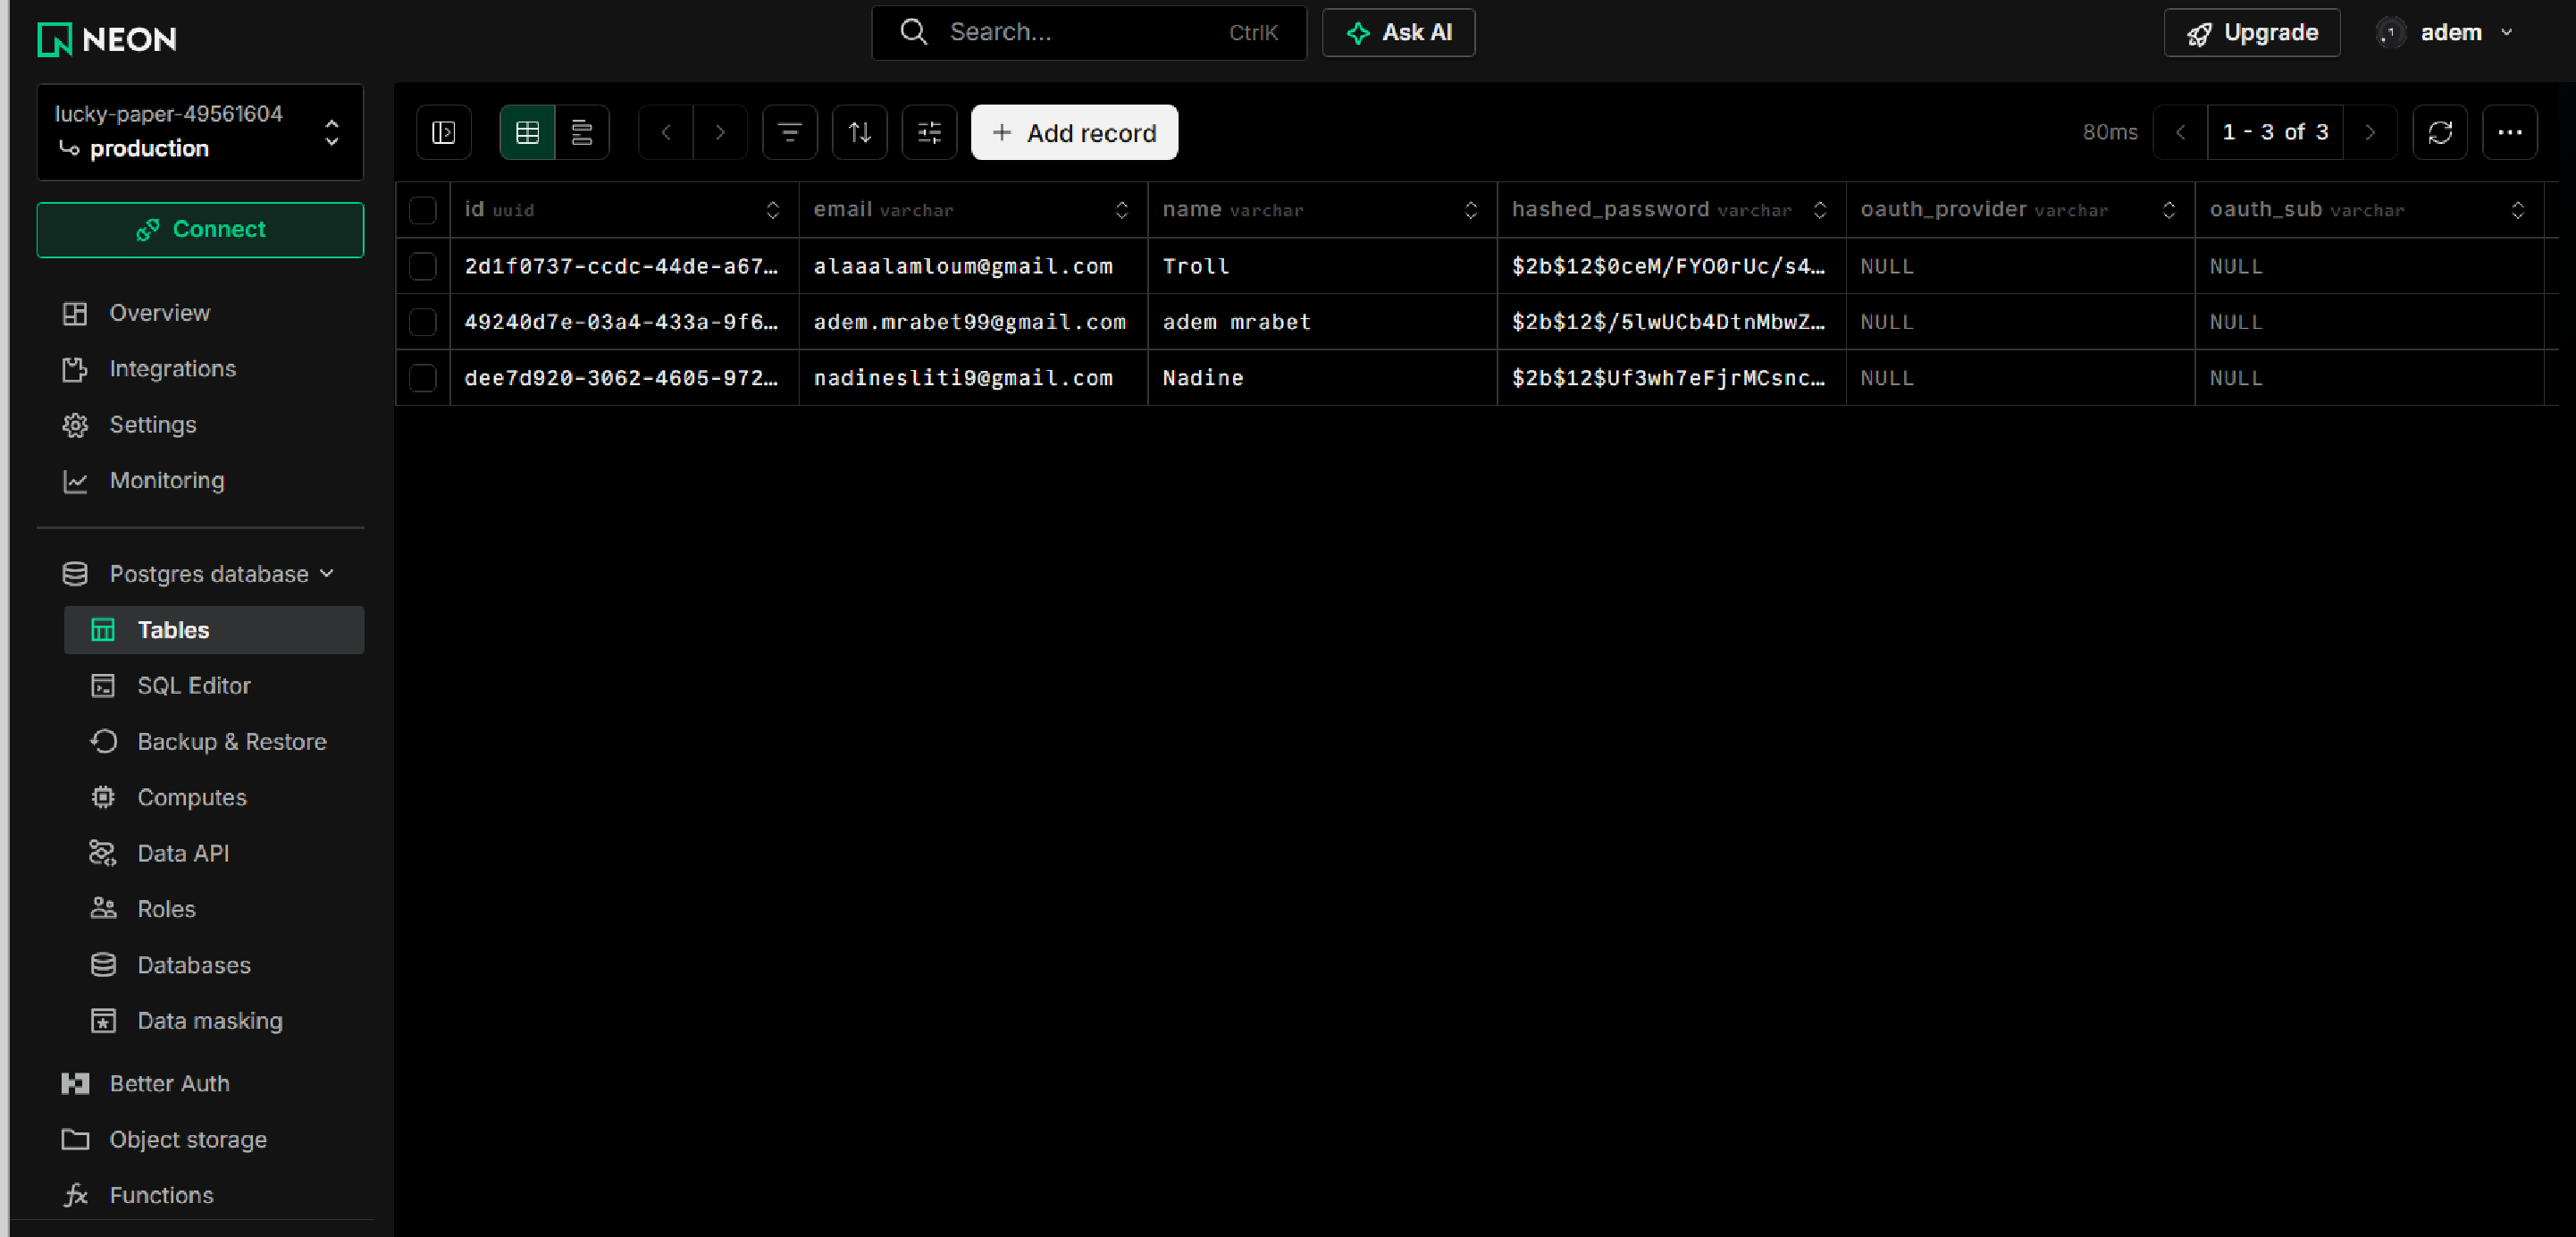
\includegraphics[width=0.98\textwidth]{figures/db-users.pdf}
\caption{Accounts table in the deployed instance. Each account carries a bcrypt
digest beginning \texttt{\$2b\$12\$}, and the federated identity columns are null for
accounts registered with a password.}
\label{fig:dbusers}
\end{figure}

\subsection{Conversations Table}

A conversation is stored as one row carrying its entire message sequence in a single JSON
column, rather than as a parent row with one child row per message. This is a deliberate
denormalisation and it deserves the scrutiny it usually attracts.

The normalised design is the textbook answer and would be correct if messages were ever
addressed individually. They are not. Every read in this application fetches a whole
conversation to display it, and every write appends to the end of one. There is no query
anywhere in the system that asks for a single message, no pagination within a conversation,
and no aggregate computed across messages. A child table would therefore contribute a join
on every read and an ordering column to maintain, in exchange for a capability nothing uses.

The second reason is that the provenance metadata attached to each answer, the resolved
identifier, the resolution method, the confidence score, the model that phrased it and the
language it was answered in, is a nested structure whose shape changed repeatedly during
development. In a column-per-field design each of those changes is a schema migration. In a
JSON column the client and the agent agree on the shape and the database stores what it is
given. Given that this metadata is only ever read back and rendered, never filtered or
joined on, the flexibility was worth more than the constraint.

The honest counterpart is stated plainly: this choice forecloses future queries such as
``how many answers fell back to the template'' without either a scan over the JSON documents
or a migration to a normalised form. That is an acceptable trade only because no such query
exists today, and it would need revisiting if the usage analytics discussed in
Section~\ref{sec:govkpi} were implemented.

Table~\ref{tab:convschema} gives the definition, and Figure~\ref{fig:dbconversations} shows
it populated.

\begin{figure}[htbp]
\centering
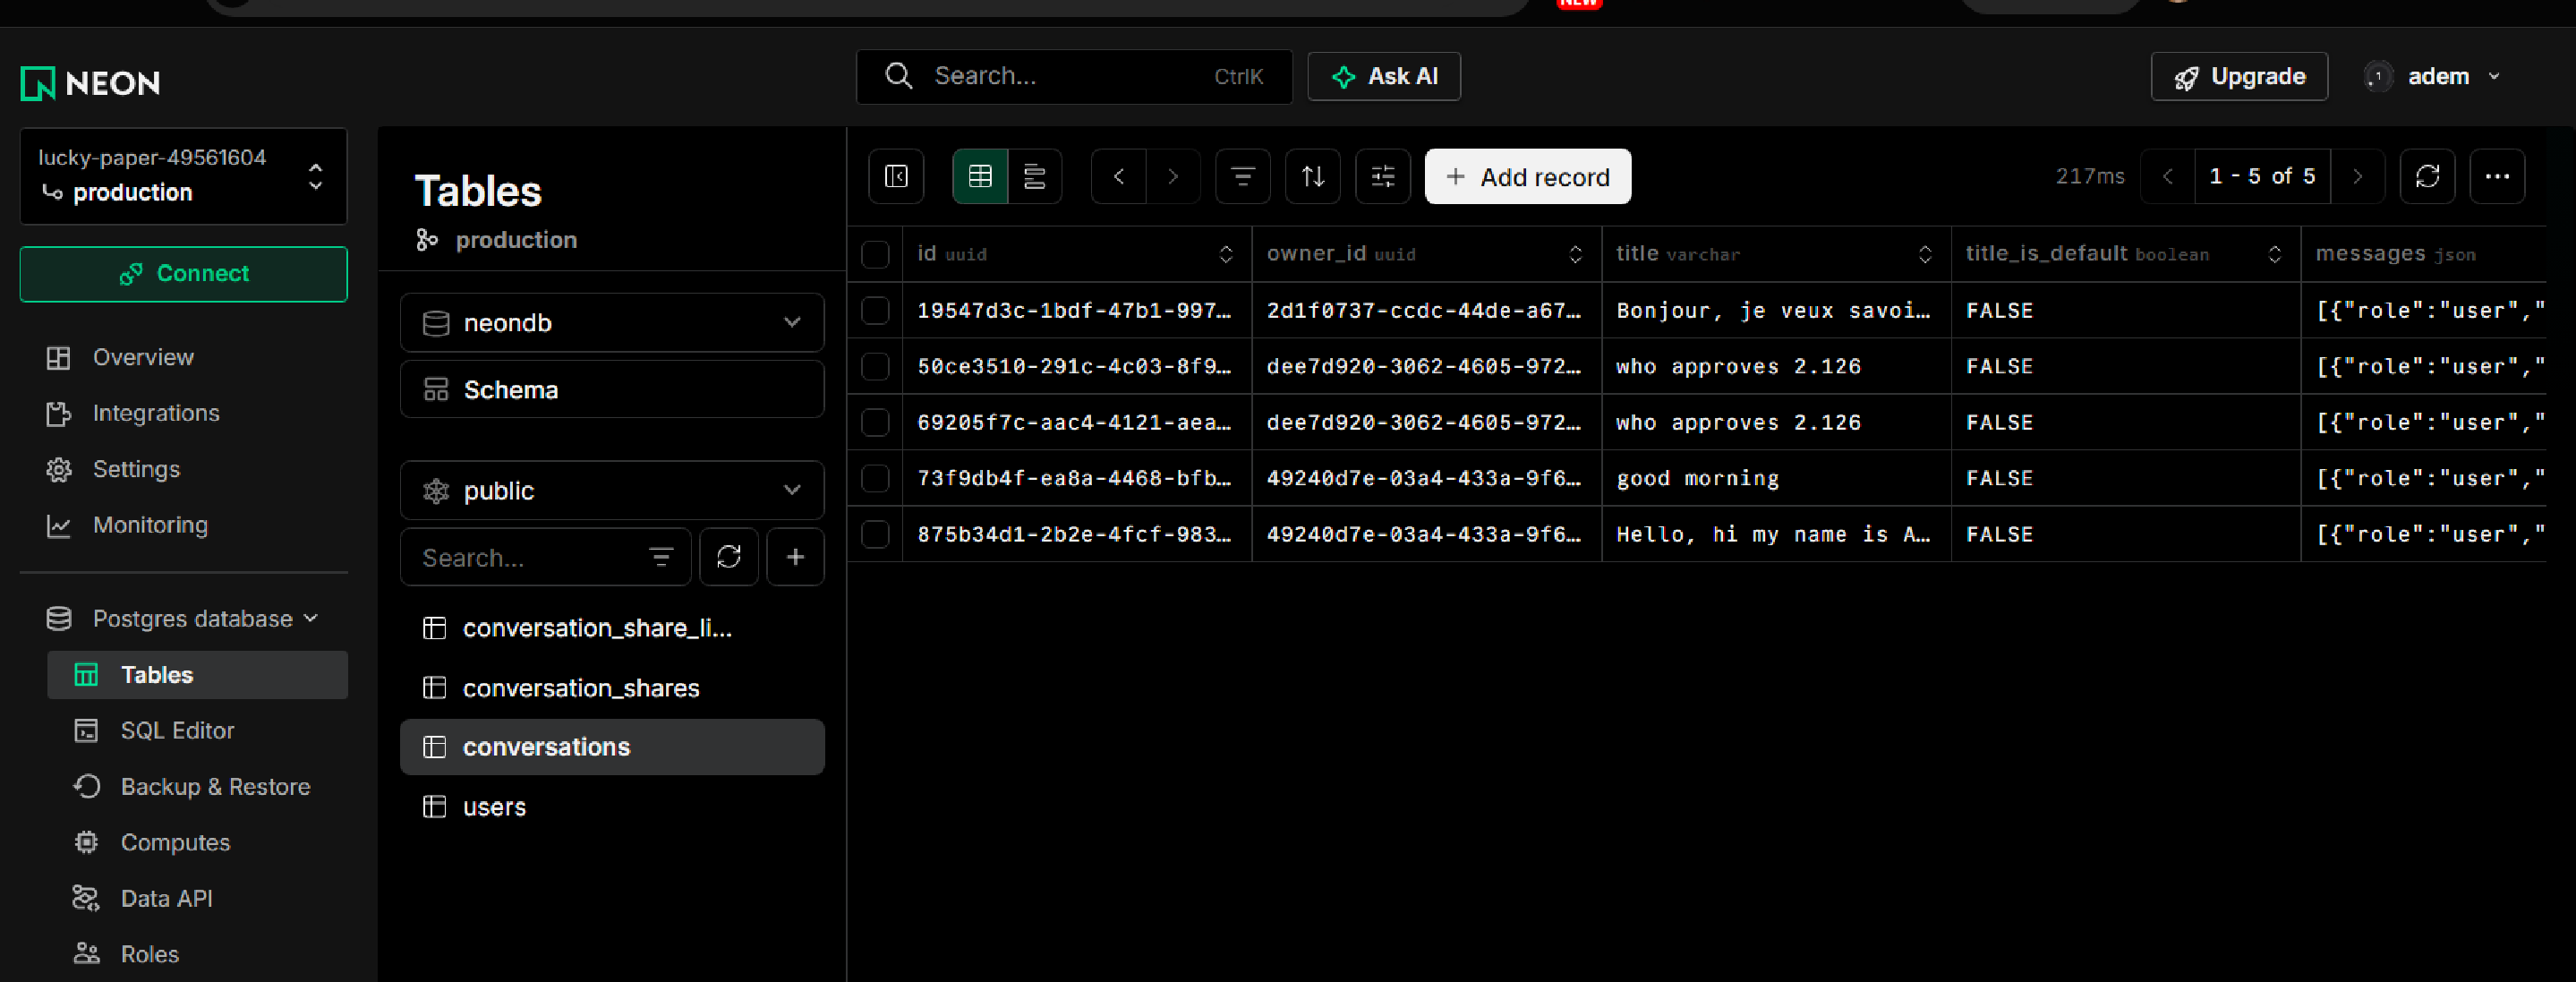
\includegraphics[width=0.98\textwidth]{figures/db-conversations.pdf}
\caption{Conversations table in the deployed instance. Each row carries a whole
thread: the owning account, the title derived from the first question, and the JSON message
column holding every exchange with its provenance metadata.}
\label{fig:dbconversations}
\end{figure}

\begin{longtable}{|p{0.22\textwidth}|p{0.16\textwidth}|p{0.52\textwidth}|}
\caption{Conversations table \texttt{conversations}.}\label{tab:convschema}\\
\hline
\rowcolor{myblue}\textcolor{white}{\textbf{Column}} & \textcolor{white}{\textbf{Type}} & \textcolor{white}{\textbf{Purpose and constraints}} \\
\hline
\endfirsthead
\hline
\rowcolor{myblue}\textcolor{white}{\textbf{Column}} & \textcolor{white}{\textbf{Type}} & \textcolor{white}{\textbf{Purpose and constraints}} \\
\hline
\endhead
\texttt{id} & UUID & Primary key. Appears in share URLs, hence random rather than sequential. \\ \hline
\texttt{owner\_id} & UUID & Foreign key to \texttt{users}, indexed. The account that created the conversation and the only one that may extend it. \\ \hline
\texttt{title} & string & Display title, defaulting to ``New chat''. \\ \hline
\texttt{title\_is\_default} & boolean & Whether the title is still the placeholder. \\ \hline
\texttt{messages} & JSON & The ordered message list, each entry carrying role, text, and provenance metadata. \\ \hline
\texttt{created\_at} & timestamp & Creation time, UTC. \\ \hline
\texttt{updated\_at} & timestamp & Maintained automatically on every write; drives sidebar ordering. \\ \hline
\end{longtable}

The \texttt{title\_is\_default} flag solves a small problem neatly enough to be worth a
sentence. A conversation should take its title from the first question asked, so that the
sidebar is navigable, but a user who renames a conversation must not have that title
overwritten by the next message. Storing the title alone cannot distinguish a placeholder
from a deliberate choice that happens to resemble one. The boolean records intent rather
than inferring it: the first message replaces the title only while the flag is set, and any
explicit rename clears it permanently.

\subsection{Sharing Tables}

Sharing is carried by two tables that do different jobs, and separating them is what keeps
authorisation coherent.

\texttt{conversation\_shares} records grants that already exist: one row per pair of
conversation and recipient. It is the single authority on who may view a conversation,
and every read path consults it. The pair is constrained unique, which makes re-sharing with
the same colleague idempotent rather than an error or a duplicate row. Two separate foreign
keys point at \texttt{users}, one for the recipient and one for the grantor, so the table
also records who extended the access rather than only that it exists.

\texttt{conversation\_share\_links} records an invitation that has not yet been accepted: a
random token, the conversation it refers to, who issued it, and when it expires, defaulting
to seven days. Crucially, a link is not itself a grant. Claiming one creates an ordinary
row in \texttt{conversation\_shares}, which means the QR-code path and the by-name path
converge on the same authorisation record, and the question of who may view a conversation
continues to have exactly one answer in the code. Had the link been treated as a credential
in its own right, every read path would have needed to check two conditions instead of one,
and the two would have drifted.

One active link is maintained per conversation. A second request for a QR code returns the
existing token rather than minting a new one, so a code already printed or already scanned
does not quietly stop working.

Table~\ref{tab:shareschema} gives both definitions, and Figure~\ref{fig:dbshares} shows a
live grant.

\begin{longtable}{|p{0.17\textwidth}|p{0.26\textwidth}|p{0.47\textwidth}|}
\caption{Two sharing tables.}\label{tab:shareschema}\\
\hline
\rowcolor{myblue}\textcolor{white}{\textbf{Table}} & \textcolor{white}{\textbf{Column}} & \textcolor{white}{\textbf{Purpose and constraints}} \\
\hline
\endfirsthead
\hline
\rowcolor{myblue}\textcolor{white}{\textbf{Table}} & \textcolor{white}{\textbf{Column}} & \textcolor{white}{\textbf{Purpose and constraints}} \\
\hline
\endhead
\texttt{conversation\_shares} & \texttt{id} & Primary key. \\ \hline
 & \texttt{conversation\_id} & Foreign key, indexed. \\ \hline
 & \texttt{shared\_with\_user\_id} & Foreign key, indexed. The account granted read access. \\ \hline
 & \texttt{shared\_by\_user\_id} & Foreign key. The account that granted it. \\ \hline
 & \texttt{created\_at} & When access was granted. \\ \hline
 & \multicolumn{2}{p{0.73\textwidth}|}{\textbf{Constraint} \texttt{uq\_conversation\_share}: (conversation, recipient) unique, making a repeat share idempotent.} \\ \hline
\texttt{conversation\_share\_links} & \texttt{id} & Primary key. \\ \hline
 & \texttt{conversation\_id} & Foreign key, indexed. \\ \hline
 & \texttt{token} & Unique and indexed. The random secret encoded into the QR image. \\ \hline
 & \texttt{created\_by\_user\_id} & Foreign key. Who issued the link. \\ \hline
 & \texttt{created\_at} & Issue time. \\ \hline
 & \texttt{expires\_at} & Expiry, defaulting to seven days after issue. \\ \hline
\end{longtable}

\begin{figure}[htbp]
\centering
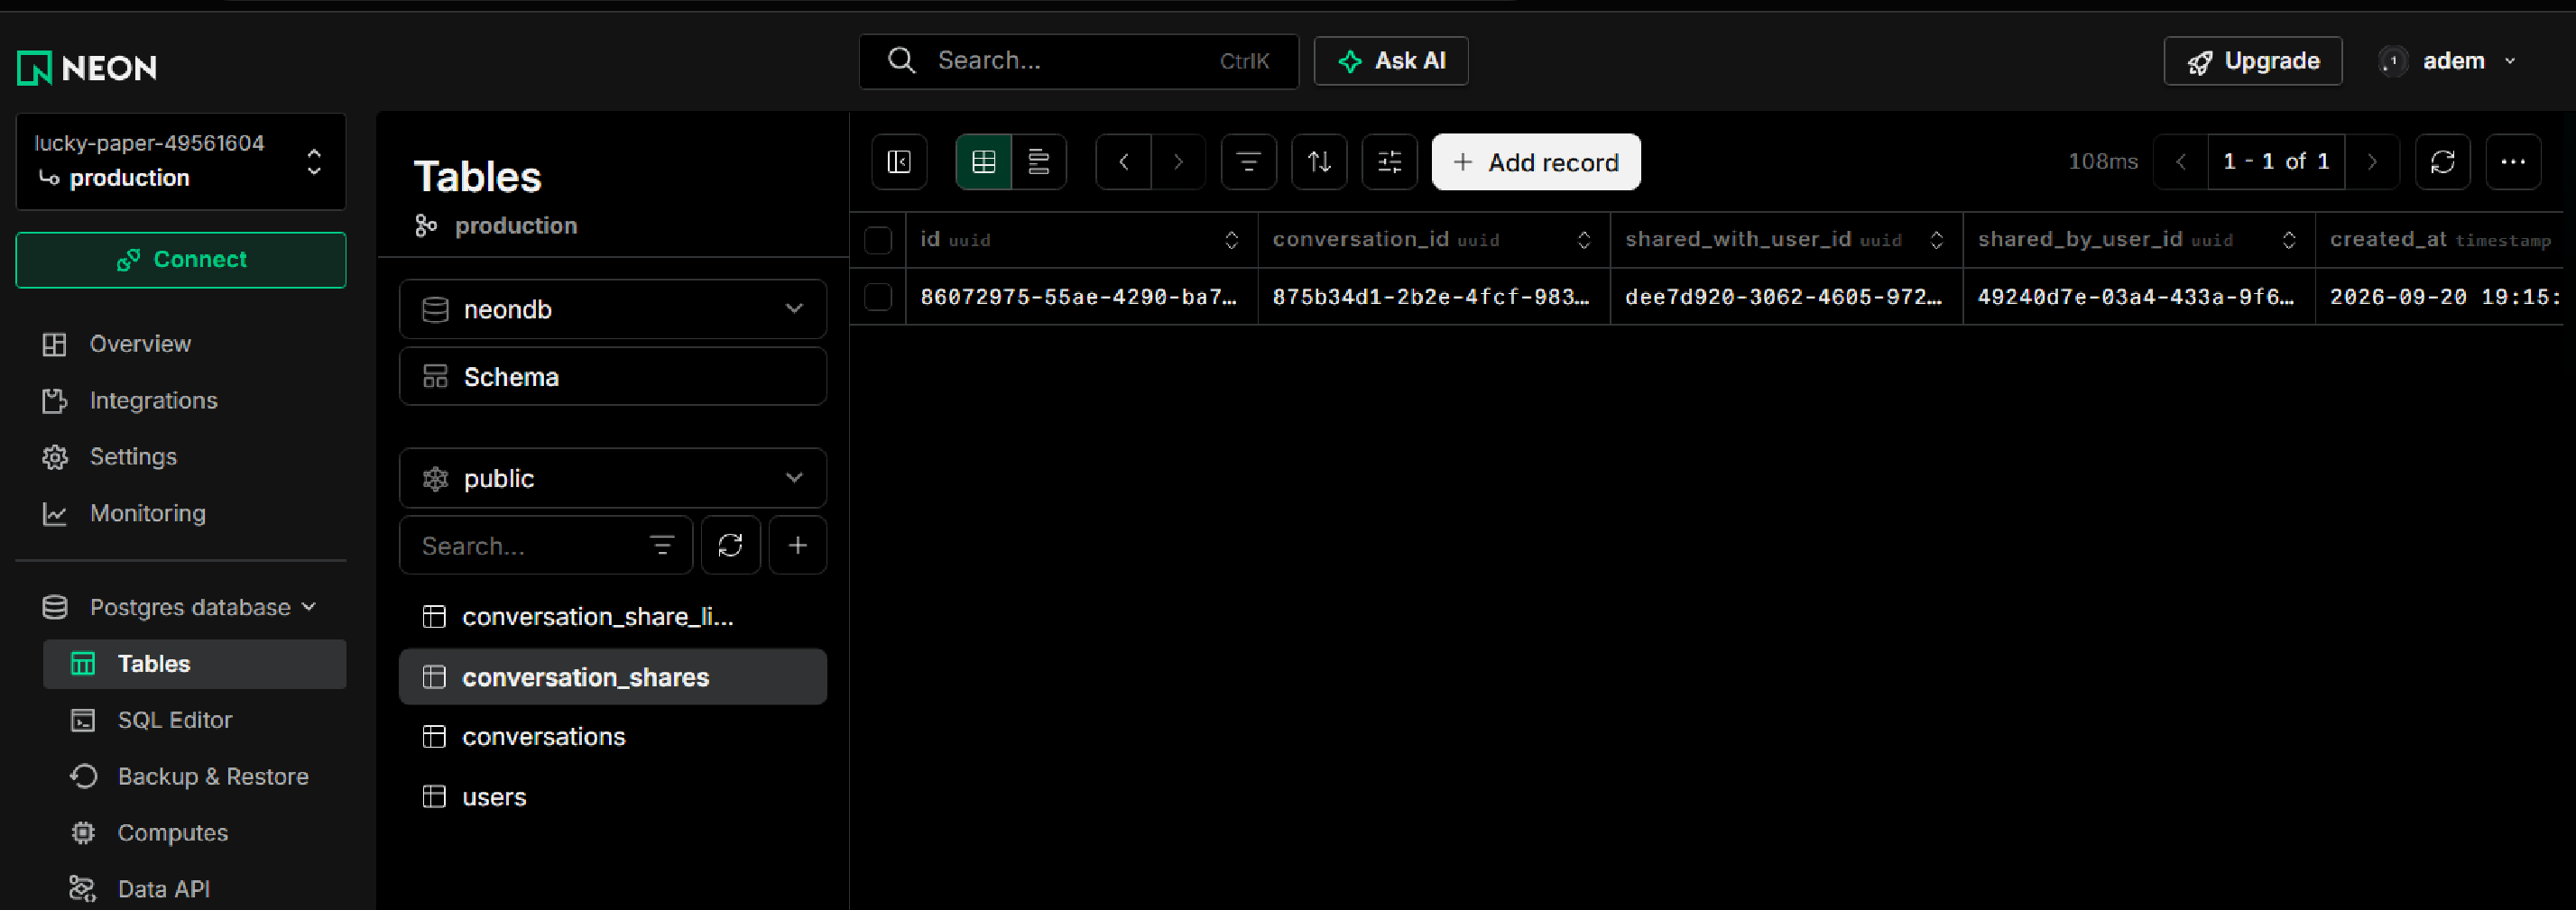
\includegraphics[width=0.98\textwidth]{figures/db-shares.pdf}
\caption{Sharing grants held in \texttt{conversation\_shares}, showing one live grant. The row names the
conversation, the account granted access, and the account that granted it.}
\label{fig:dbshares}
\end{figure}

\subsection{Referential Integrity and Deletion}

Both sharing tables are declared as dependants of the conversation with delete-orphan
cascade, so removing a conversation removes its grants and its outstanding links in the same
operation. This matters more than ordinary tidiness. Without the cascade, deleting a
conversation would leave grant rows pointing at an identifier that no longer resolves, and an
outstanding share link would remain valid in the sense that its token still existed and had
not expired. Access-control records that outlive the thing they protect are precisely the
kind of residue that later produces a security incident, so the lifetime of a grant is bound
to the lifetime of its conversation at the schema level rather than in application code that
might be bypassed.

One implementation detail is worth recording because it caused a real error. The share table
holds two foreign keys into \texttt{users}, and the mapper cannot infer which one a given
relationship traverses when more than one candidate exists; both relationships therefore
declare their join column explicitly. The error surfaces at mapper configuration time rather
than at query time, which is the preferable failure, but it is opaque enough on first
encounter to be worth naming here.

\section{Access Control}

Ownership is the concept this whole section serves: nothing about persistence or sharing
means anything until the system can say whose conversation it is looking at.
Figure~\ref{fig:applogin} shows the sign-in screen the decisions below sit behind.

\begin{figure}[htbp]
\centering
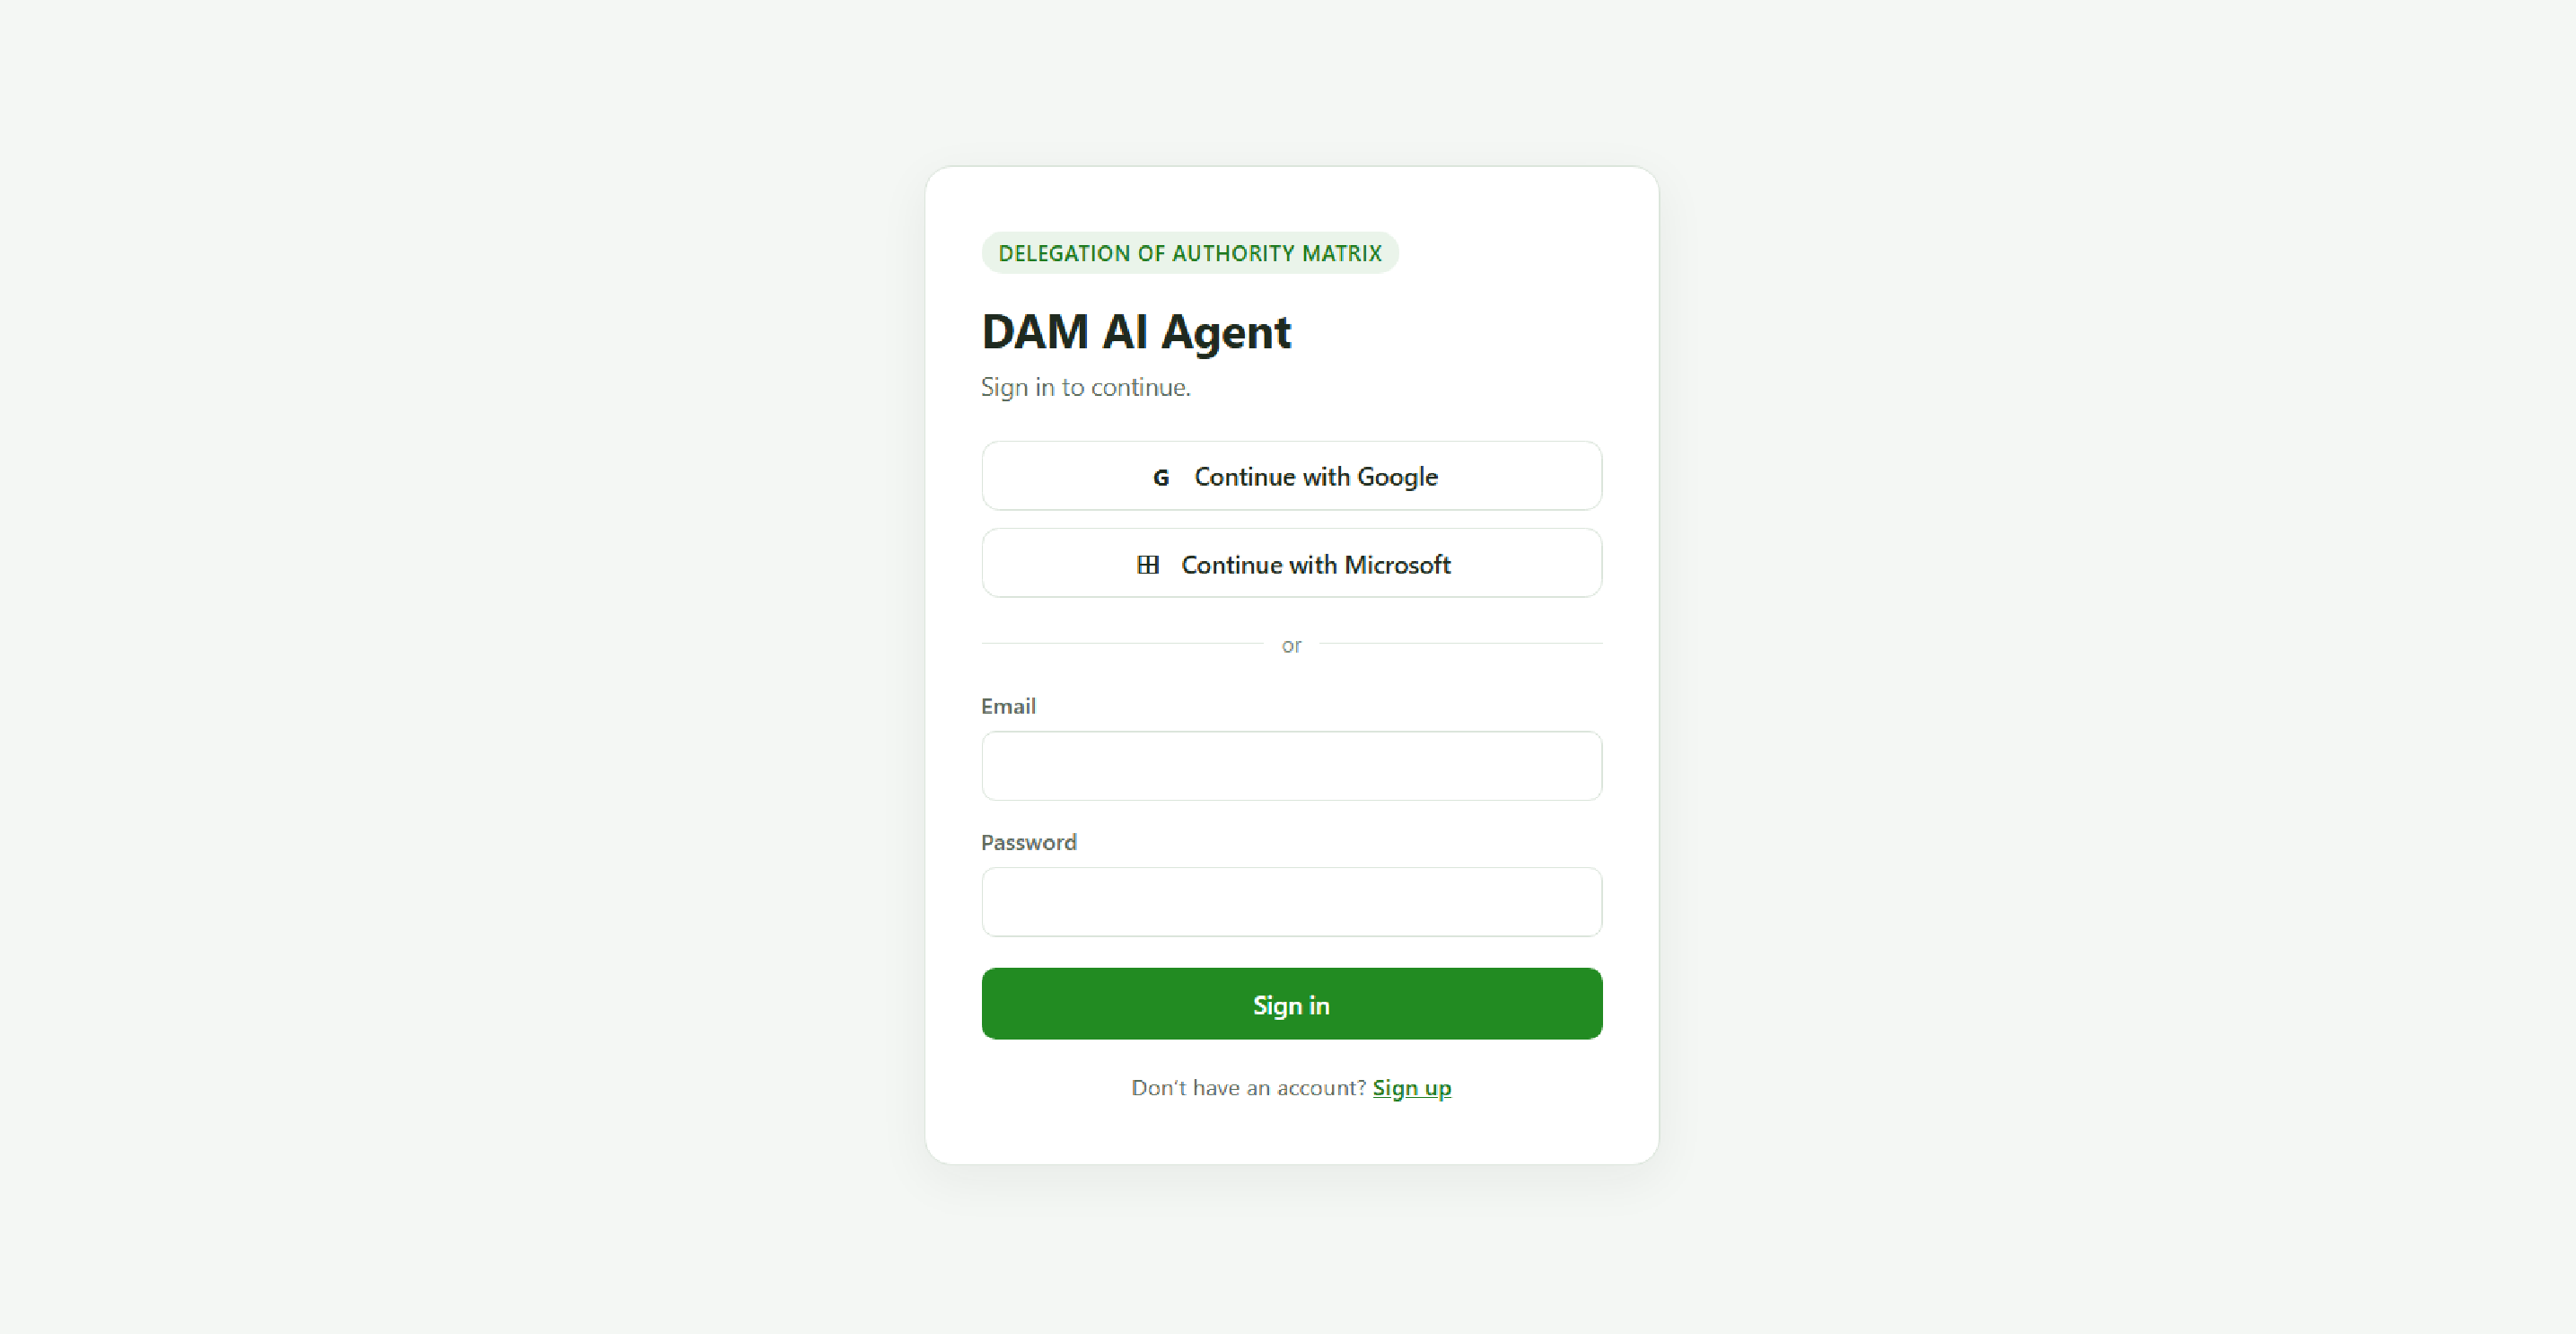
\includegraphics[width=0.55\textwidth]{figures/app-login.pdf}
\caption{Sign-in screen, offering federated sign-in through Google or Microsoft alongside
the email-and-password form.}
\label{fig:applogin}
\end{figure}

\subsection{Why Authentication Was Necessary}

The first version of this system had no accounts. Anyone reaching the service could ask
questions, and conversations lived in the browser's own storage. That was adequate while the
system did one thing, and it stopped being adequate the moment conversations needed to be
persisted and shared, for a reason that is structural rather than incidental: sharing
requires ownership, ownership requires identity, and identity requires authentication. There
is no way to grant a colleague access to something that belongs to nobody.

A second reason is specific to this subject matter. The analytics layer aggregates the
delegation structure of the institution, which is organisationally sensitive in a way that a
single lookup is not, and restricting it requires being able to tell who is asking.

\subsection{Password Storage}

Passwords are never stored in a form from which the original can be recovered. Each account
holds a bcrypt digest, produced through the passlib library, and verification re-derives a
digest from the submitted password and compares the two. Bcrypt was chosen over a
general-purpose cryptographic hash for reasons worth setting out, since the distinction is
frequently elided.

A hash such as SHA-256 is designed to be fast, which is the correct property for verifying
file integrity and precisely the wrong one for storing passwords: speed is exactly what an
attacker holding a stolen database wants, since it lets them test billions of candidate
passwords per second on commodity hardware. Bcrypt is deliberately slow and, more
importantly, adjustably slow. Its cost parameter sets the number of key-expansion rounds as a
power of two, and raising it by one doubles the work required both for a legitimate
verification and for every guess an attacker makes. The digests in this system carry a cost
of twelve, meaning $2^{12}$ rounds, which is visible in the \texttt{\$2b\$12\$} prefix of
every stored value in Figure~\ref{fig:dbusers}. The parameter is stored alongside the digest
rather than fixed in code, so the cost can be raised as hardware improves and existing
accounts continue to verify against their original setting until their next successful login.

Bcrypt also salts each password individually and stores the salt in the same field. The
consequence is that two accounts choosing the same password hold entirely different digests,
which defeats both precomputed rainbow tables and the simpler attack of noticing that two
rows share a value and therefore share a password.

The interaction between password storage and federated accounts is the property described
earlier: an account authenticated through a provider carries no digest at all, and the login
endpoint refuses it before any comparison is attempted.

\subsection{Token Design}

Authentication is stateless. A successful sign-in returns a signed JSON Web
Token\citep{rfc7519}, and the client presents it in the \texttt{Authorization} header of
every subsequent request. Table~\ref{tab:jwtclaims} lists what the token asserts.

\begin{longtable}{|p{0.14\textwidth}|p{0.30\textwidth}|p{0.46\textwidth}|}
\caption{Claims carried by the access token.}\label{tab:jwtclaims}\\
\hline
\rowcolor{myblue}\textcolor{white}{\textbf{Claim}} & \textcolor{white}{\textbf{Value}} & \textcolor{white}{\textbf{Why it is present}} \\
\hline
\endfirsthead
\hline
\rowcolor{myblue}\textcolor{white}{\textbf{Claim}} & \textcolor{white}{\textbf{Value}} & \textcolor{white}{\textbf{Why it is present}} \\
\hline
\endhead
\texttt{sub} & Account UUID & Identifies the caller. Every ownership check resolves from this. \\ \hline
\texttt{email} & Address & Lets the interface show the signed-in account without an extra request. \\ \hline
\texttt{role} & \texttt{analyst} or \texttt{administrator} & Carries the authorisation decision, avoiding a lookup on every request. \\ \hline
\texttt{iat} & Issue time & Establishes token age. \\ \hline
\texttt{exp} & Issue time plus eight hours & Bounds the damage a leaked token can do. \\ \hline
\end{longtable}

The token is signed HS256\citep{rfc7515}, a keyed signature using a secret held only by the
server. Signing establishes integrity, not confidentiality: the claims are encoded, not
encrypted, and anyone holding the token can read them. Nothing secret is therefore placed in
it. What signing guarantees is that a client cannot alter a claim, and the claim that matters
is \texttt{role}: without a signature, elevating oneself to administrator would be a matter
of editing a string.

The signing secret is read from the environment with no fallback default, so a deployment
that has not configured one fails immediately at startup rather than silently signing tokens
with a value an attacker could guess from the source. Failing loudly at boot is the correct
behaviour for a misconfiguration of this class.

Expiry is eight hours, chosen to span a working day. The trade-off is explicit: a shorter
window would force repeated sign-ins during ordinary use, and a longer one would leave a
usable credential in a browser long after the person had finished. Because verification is
stateless, a token cannot be revoked before it expires, which is the cost of not consulting
the database on every request. For this application that cost is acceptable; a system holding
higher-value operations would need a revocation list and the lookup that comes with it.

On the client the token is held in session storage rather than local storage. Both are
readable by any script executing on the page, so the distinction is not about resisting
script access; it is about lifetime. Session storage is cleared when the tab closes, whereas
local storage persists indefinitely, leaving a valid credential on a shared or unattended
machine long after the user believed they had finished. The cost is that closing the tab
requires signing in again, which was judged the right trade for a system holding governance
information.

\subsection{Federated Sign-In}

Two federated paths exist alongside the password form, through Google and through Microsoft.
The motivation is institutional rather than technical: staff at an organisation of this kind
already hold a corporate directory account, and requiring a separate password adds a
credential to be managed, forgotten, reused, or written down, while removing the ability of
the institution to revoke access centrally when someone leaves.

Both providers are integrated through OpenID Connect rather than by hand-coded calls to
provider endpoints. The client is configured with a discovery document URL, and the endpoints,
signing keys and supported parameters are retrieved from the provider at runtime. This matters
for durability: a provider rotating its signing keys or relocating an endpoint does not break
the integration, because nothing about those details is hardcoded. The requested scope is the
minimum the application needs, namely the identity token plus the address and display name.
The Microsoft integration additionally accepts a tenant identifier, defaulting to the
multi-tenant endpoint, so that the same build can be pointed at a single institutional
directory by configuration alone.

Both providers are registered only when their credentials are present in the environment. An
instance configured with neither still starts and still serves password sign-in, which keeps
local development and the test suite free of any dependency on external identity services.

\subsection{Resolving a Federated Identity to an Account}

The step where a provider's response becomes a local account is the most security-sensitive
part of the flow, and the order of the lookups is the substance of it.

The account is located first by the pair of provider and subject identifier, the provider's
own immutable handle for that person, and never by email address alone. This ordering is
deliberate. Email addresses are not stable identifiers: an organisation may reassign a
departed employee's address to a new hire, and a person may change their own address at the
provider. A system matching on email alone would hand the new holder of a recycled address
the previous holder's account and every conversation in it. Matching on the subject
identifier makes that impossible, because the identifier is never reissued.

Only when no account carries that provider identity does the resolution fall back to email,
and then only to link the provider identity onto an existing account rather than to
authenticate against it. This is what lets a user who registered with a password later sign
in through Google and arrive at the same account rather than a duplicate. The account is
created fresh only when both lookups fail.

The uniqueness constraint on the provider-and-subject pair enforces the invariant at the
database level, so a defect in this logic cannot produce two local accounts claiming the same
provider identity.

Figure~\ref{fig:authflow} lays out the same decision as a flowchart, since the order in
which the three checks run is the part of this logic most likely to be got wrong by a
future change.

\begin{figure}[htbp]
\centering
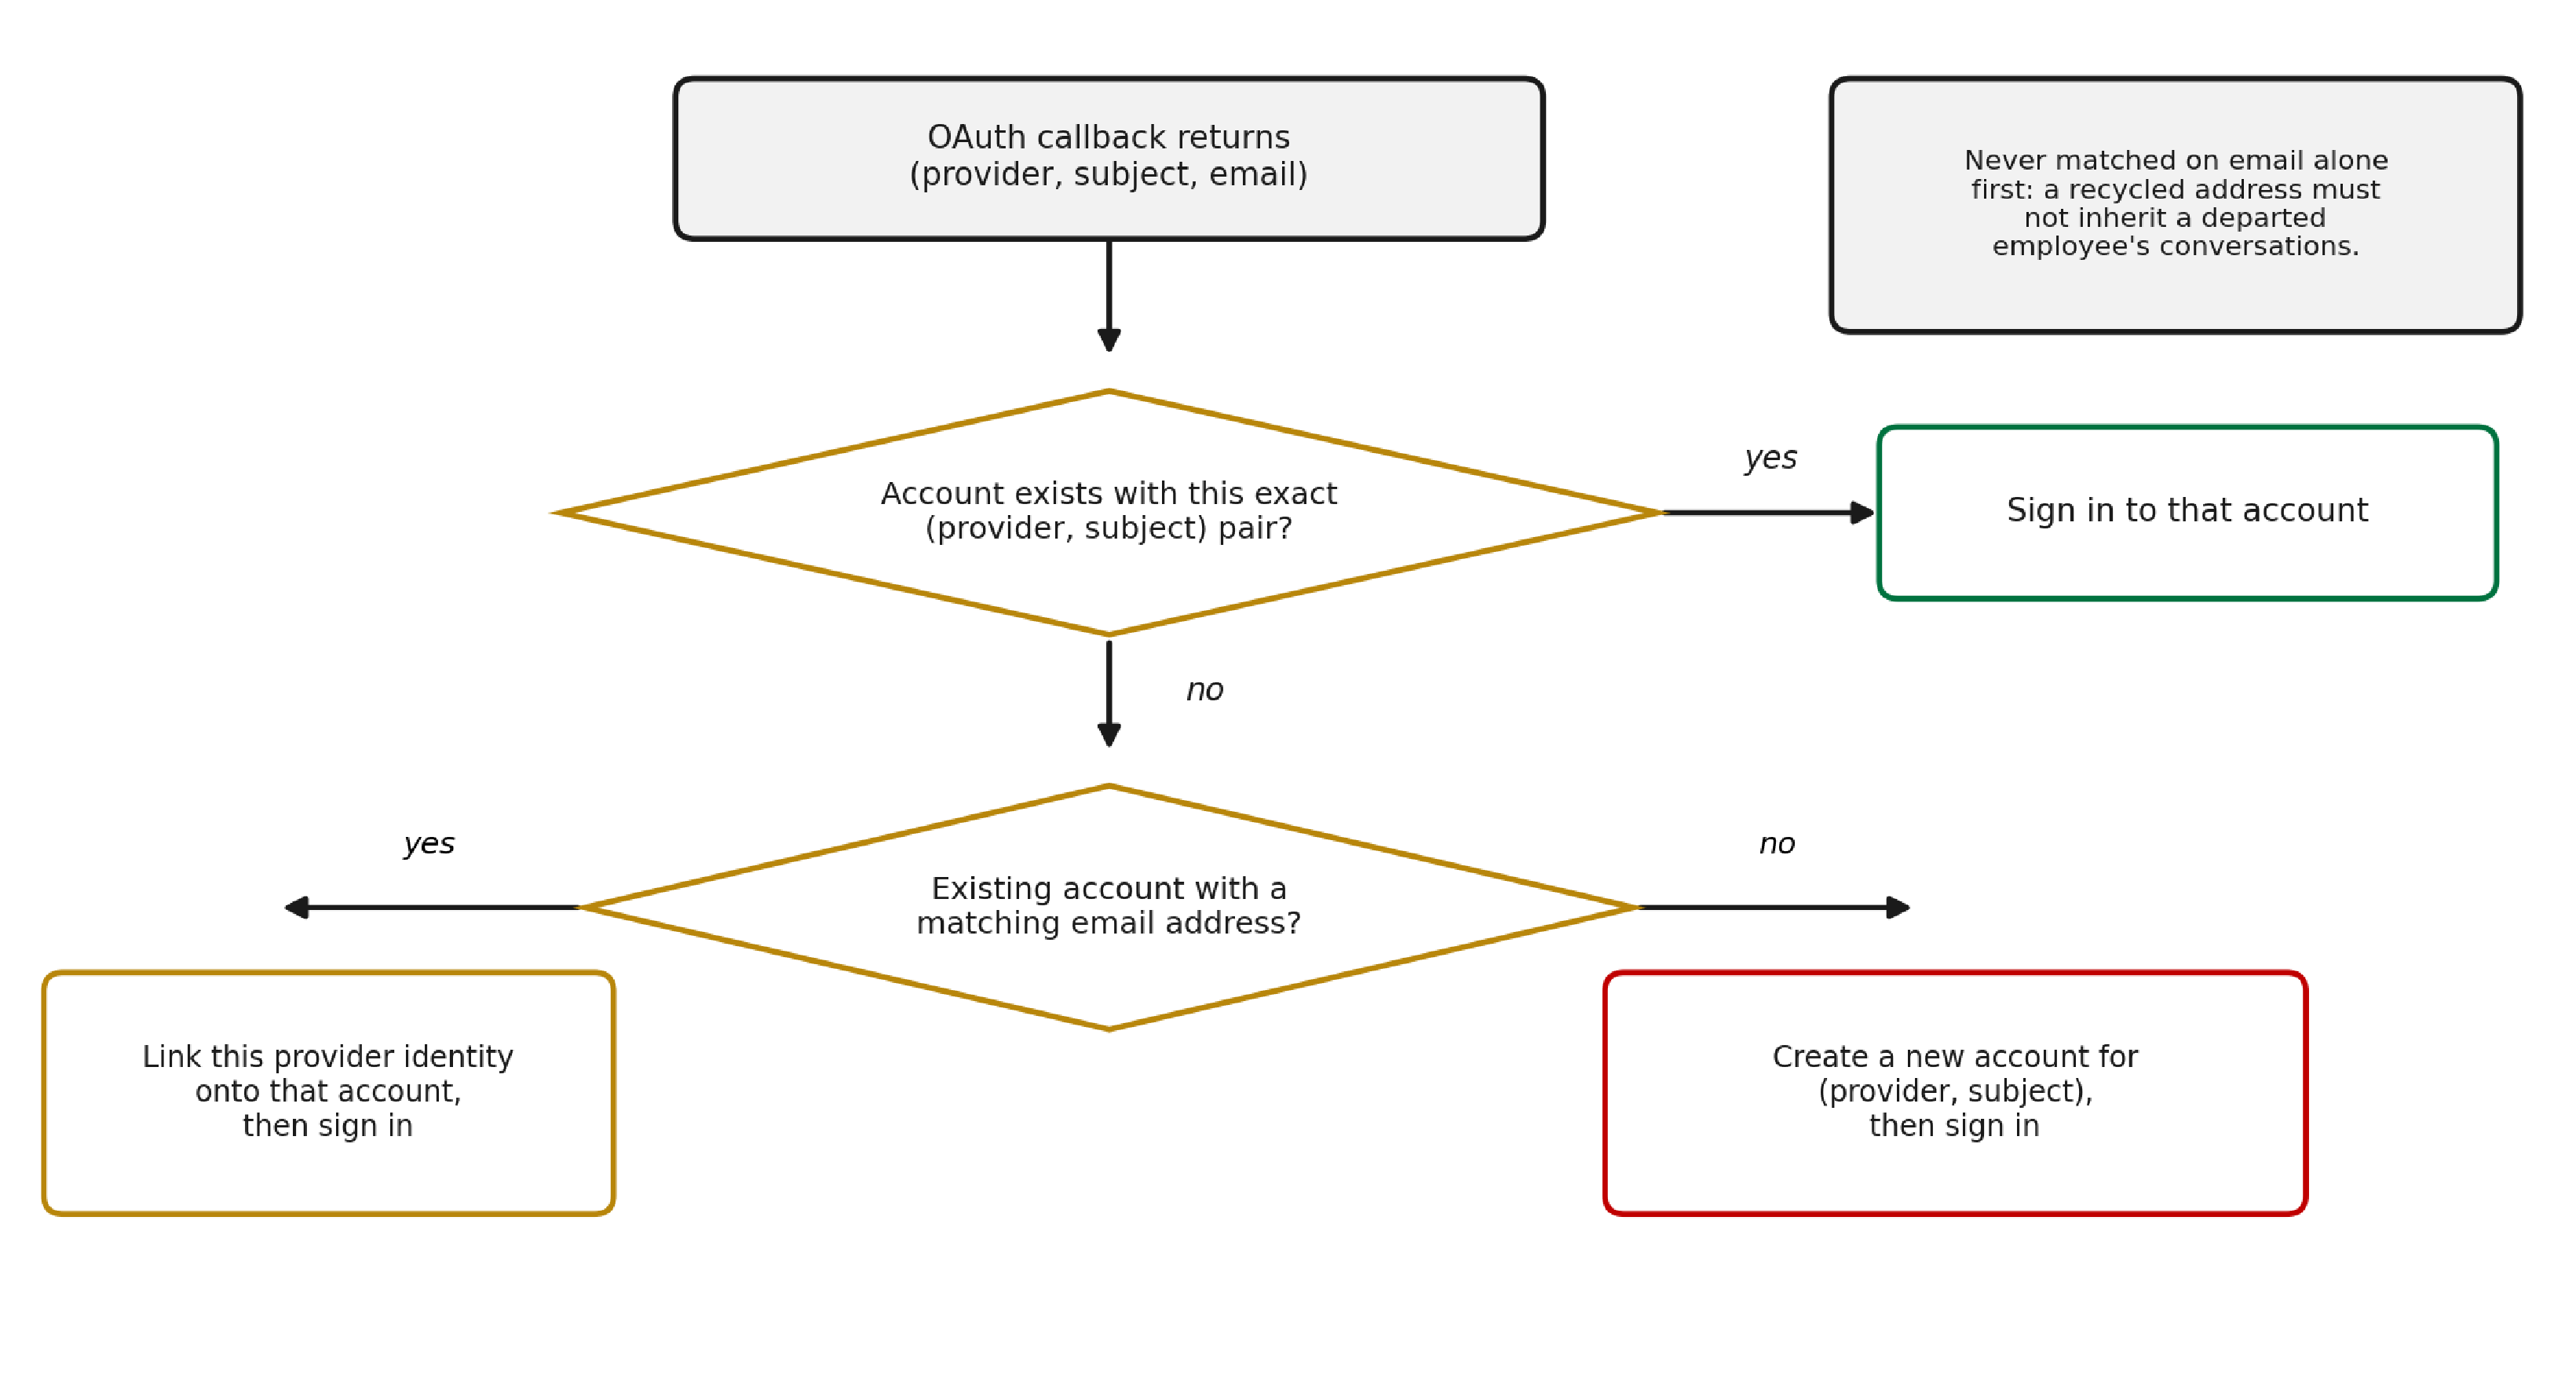
\includegraphics[width=0.92\textwidth]{figures/fig-authflow.pdf}
\caption{Resolving a federated identity to a local account. The provider-and-subject pair is
checked first and email is consulted only as a fallback for linking, never for
authentication.}
\label{fig:authflow}
\end{figure}

\subsection{Roles and Authorisation}

Two roles are defined. An \textbf{analyst} may ask questions, attach documents, and own and
share conversations. An \textbf{administrator} may additionally open the analytics dashboard.
The distinction reflects the sensitivity difference described earlier: an individual
conversation reveals what one person asked, whereas the dashboard aggregates the institution's
delegation structure.

Authorisation is enforced server-side as a dependency on the protected routes rather than by
hiding controls in the interface. An analyst who constructs the request by hand is refused
exactly as one who clicks, which is the only enforcement that means anything; a hidden button
is a usability affordance, not a control.

The first account created on an empty database becomes an administrator, which solves the
bootstrap problem of needing an administrator before one can be appointed. This is recorded as
a deliberate convenience rather than a complete design: promoting a second administrator still
requires a direct database edit, and a production deployment would want an administrative
interface for it.

\subsection{Hardening the Sign-In Path}

Three further protections apply specifically to authentication, and
Table~\ref{tab:threatmodel} sets out what each defends against.

Failed attempts are rate-limited by source address within a rolling five-minute window, which
raises the cost of credential stuffing from free to impractical without locking out a
legitimate user who has mistyped a password twice.

A failed sign-in returns one generic message regardless of whether the account exists. The
temptation to be helpful here, by saying that no account was found, produces an oracle that
converts a list of institutional email addresses into a list of confirmed users. The
implementation is careful on a related point: the same generic refusal is returned when an
account exists but has no password because it is federated, so the response does not
distinguish that case either.

A minimum password length of eight characters is enforced at registration. This is a weak
control on its own and is stated as such; it raises the floor without pretending to establish
password quality.

\begin{longtable}{|p{0.30\textwidth}|p{0.56\textwidth}|}
\caption{Authentication threats and the corresponding mitigation.}\label{tab:threatmodel}\\
\hline
\rowcolor{myblue}\textcolor{white}{\textbf{Threat}} & \textcolor{white}{\textbf{Mitigation in this system}} \\
\hline
\endfirsthead
\hline
\rowcolor{myblue}\textcolor{white}{\textbf{Threat}} & \textcolor{white}{\textbf{Mitigation in this system}} \\
\hline
\endhead
Database disclosure exposing passwords & Only salted bcrypt digests at cost twelve are stored; federated accounts hold no digest at all. \\ \hline
Offline brute-force against stolen digests & Bcrypt's cost parameter makes each guess expensive, and the parameter can be raised without a migration. \\ \hline
Rainbow-table attack & Per-password salts make precomputation useless and hide the fact that two accounts share a password. \\ \hline
Account enumeration & One generic refusal for unknown account, wrong password, and federated account alike. \\ \hline
Credential stuffing & Rate limiting per source address over a rolling window. \\ \hline
Privilege escalation by editing a token & The role claim is covered by the HS256 signature; any alteration invalidates the token. \\ \hline
Credential left on a shared machine & Tokens held in session storage, discarded when the tab closes, and expiring after eight hours regardless. \\ \hline
Conversation URL enumeration & Random UUID identifiers rather than sequential integers, with the ownership check retained as well. \\ \hline
Recycled email address inheriting an account & Federated identities resolved by immutable provider subject identifier before email is ever consulted. \\ \hline
Stale access after a conversation is deleted & Grants and outstanding links removed by database cascade with the conversation itself. \\ \hline
Misconfigured deployment signing with a default secret & The signing secret has no default; a deployment without one fails at startup. \\ \hline
\end{longtable}

\section{Conversation Interface}

With sign-in in place, what a signed-in user actually does becomes the subject: ask a
question, dictate it instead of typing, attach a document to be questioned separately from
the DAM, or read the interface in their own language. Each input mode runs through the same
underlying answer pipeline from Chapter~\ref{ch:agent}, since none of them change what an
answer is, only how the question reaches it.

\subsection{Asking a Question}

The chat page is the primary interface. A question is typed or dictated, and the answer
returns accompanied by the metadata that makes it checkable: the resolved activity
identifier, the resolution method, the confidence score where one applies, whether a
language model phrased the response, and the language the answer is written in.
Figure~\ref{fig:appchat} shows an exchange in which the agent first declines to guess at
an under-specified question and offers candidate activities, then answers the follow-up
by identifier at full confidence.

\begin{figure}[htbp]
\centering
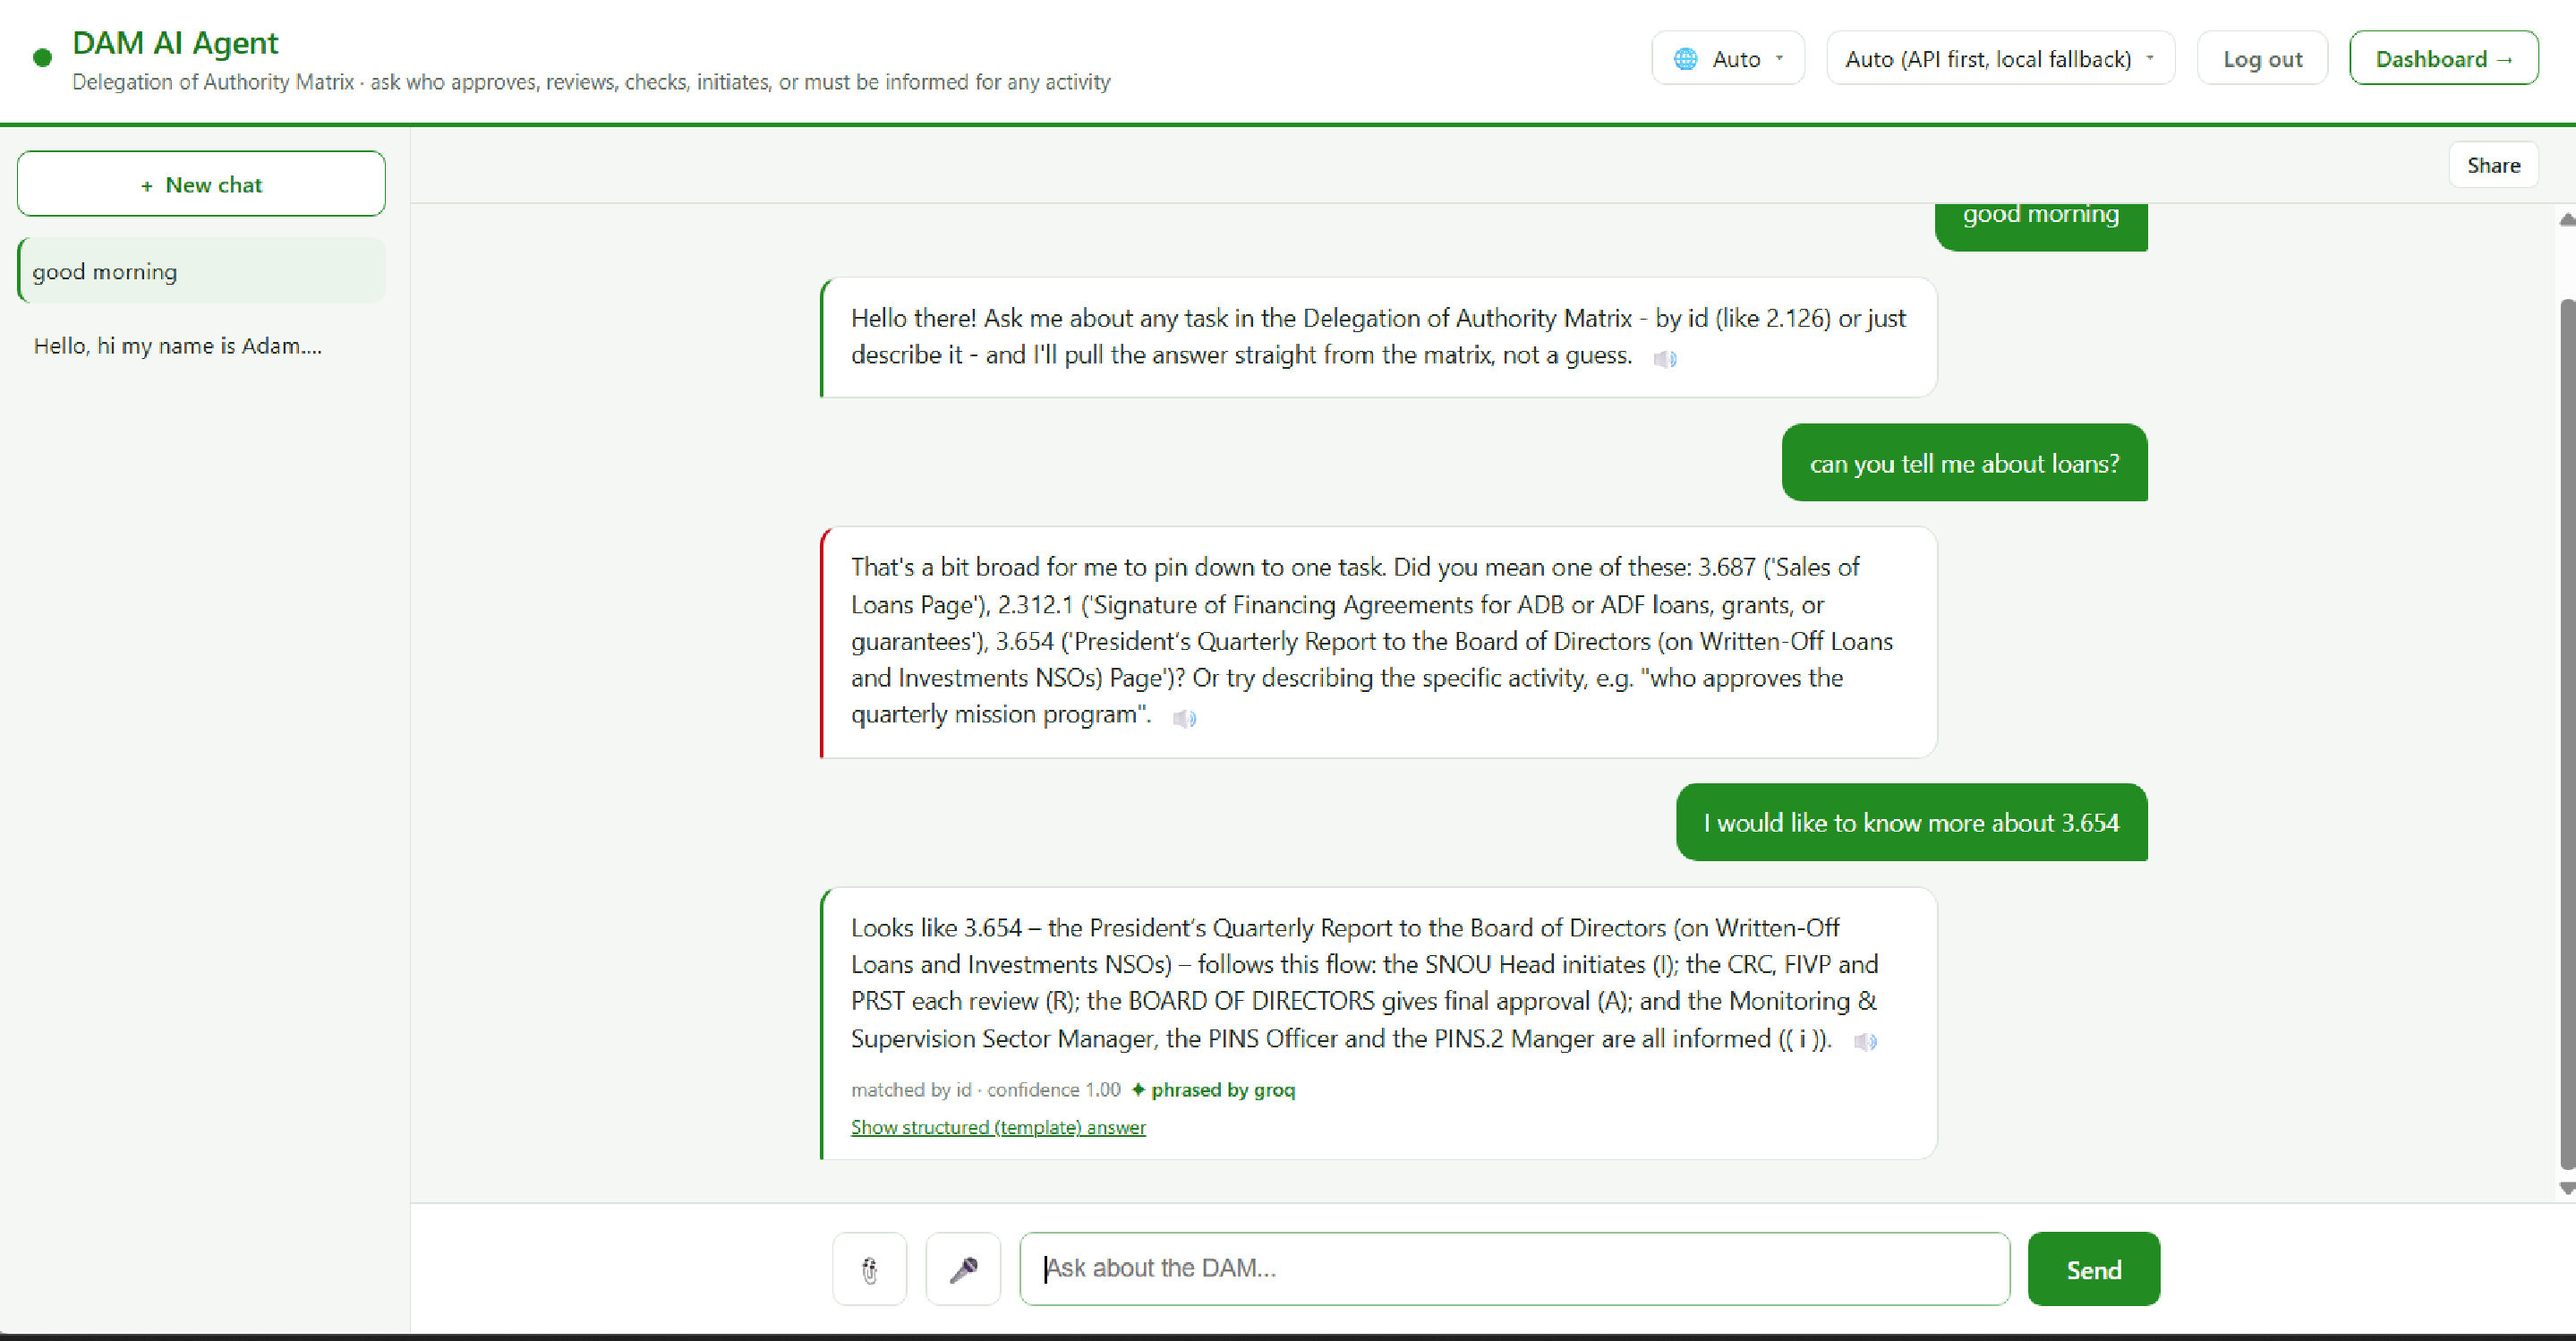
\includegraphics[width=0.95\textwidth]{figures/app-chat.pdf}
\caption{Conversation interface. The first answer refuses an under-specified question
and offers candidates rather than guessing; the second resolves by identifier at
confidence 1.0 and carries its provenance beneath the answer.}
\label{fig:appchat}
\end{figure}

Header controls select the language model mode, as set out in Table~\ref{tab:llm},
including switching it off entirely, and select the answer language. Beneath any answer a
model has phrased, a control reveals the deterministic template answer underneath it, so a
user can compare the readable sentence against the unembellished statement of what the
matrix records. This control is the interface expression of the architectural separation
argued for in Chapter~\ref{ch:agent}: the two layers remain visibly distinct at the point
of use, rather than being merged into a single authoritative-sounding paragraph.

The landing page, shown in Figure~\ref{fig:applanding}, states the same distinction before
a user has asked anything, since the difference between an answer retrieved from a
structured source and an answer generated from a document is precisely the expectation a
new user arrives with.

\begin{figure}[htbp]
\centering
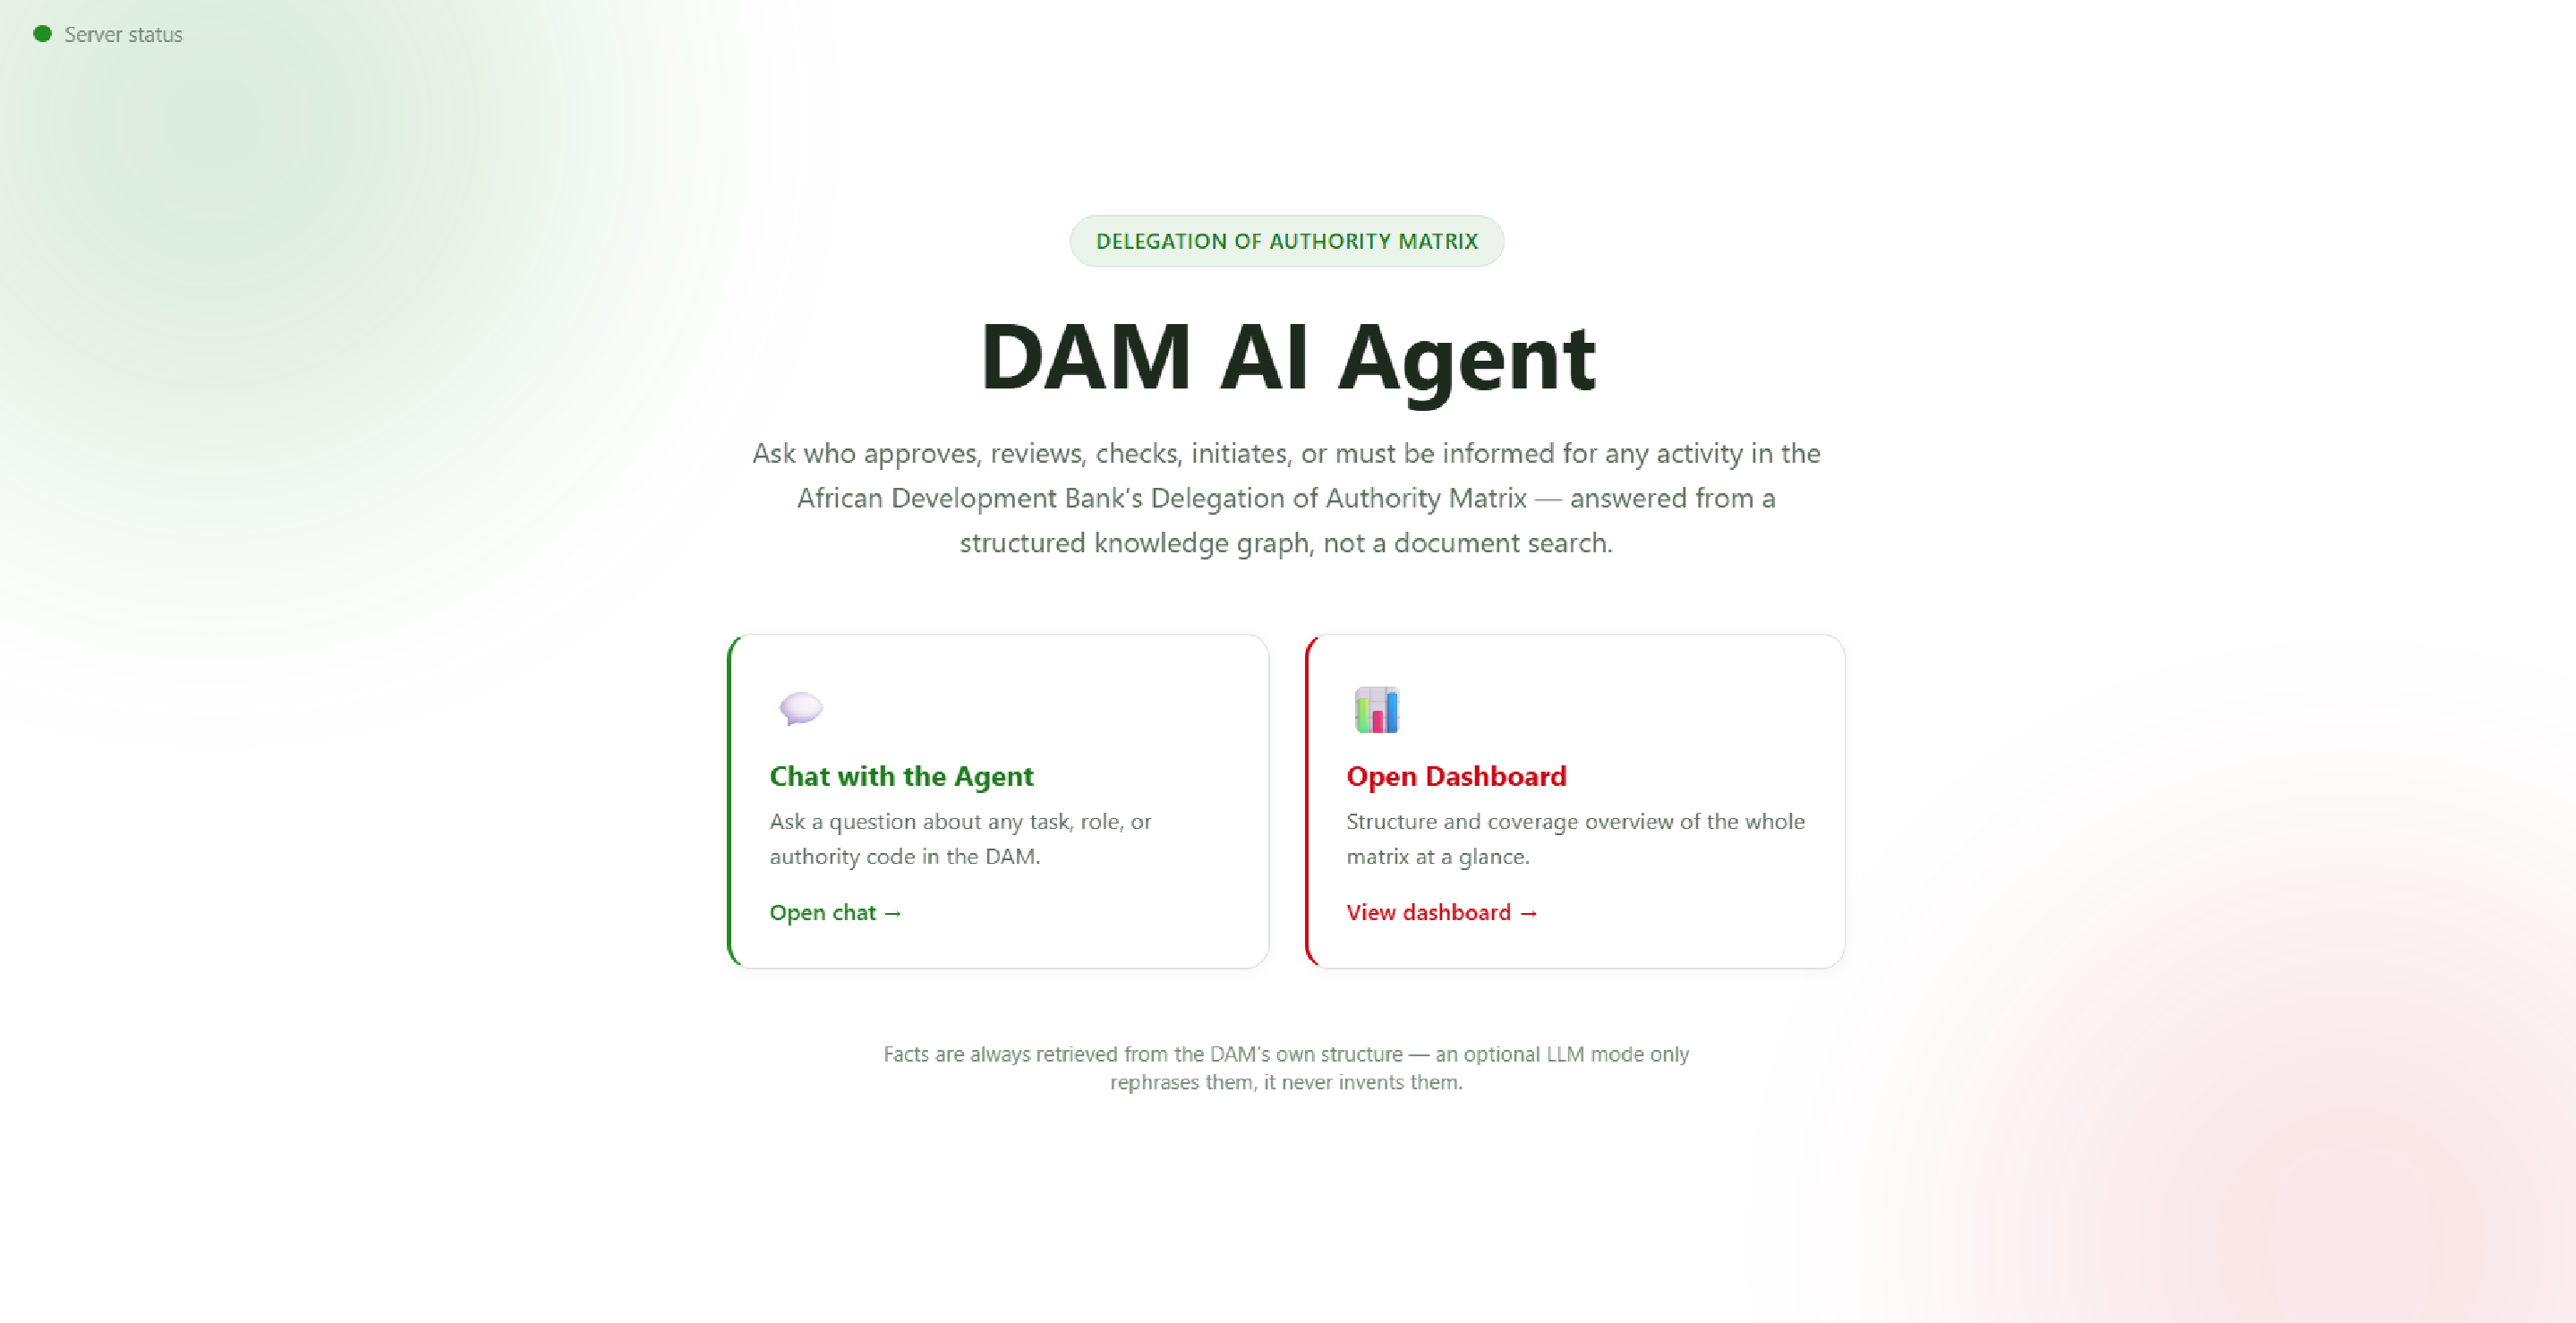
\includegraphics[width=0.96\textwidth]{figures/app-landing.pdf}
\caption{Landing page, which states the grounding guarantee before any question is
asked.}
\label{fig:applanding}
\end{figure}

\subsection{Voice Input}

A question may be dictated instead of typed. The composer exposes a microphone control
which captures audio in the browser through the \texttt{MediaRecorder} interface and posts
the resulting clip to a transcription endpoint, where it is transcribed by a hosted
Whisper model and returned as text. Transcription is therefore server-mediated rather than
performed in the browser, which keeps behaviour identical across browsers that implement
on-device speech recognition inconsistently or not at all.

One design decision is deliberate and easy to miss. The returned transcript is placed into
the input field for review rather than submitted automatically. Speech recognition
performs poorly on institutional acronyms and on numeric activity identifiers, which is
exactly what these questions contain; a user who never sees the transcript cannot correct
an identifier that was misheard. Routing the transcript through the input field also means
it passes through the deterministic typo correction described in
Chapter~\ref{ch:agent} before retrieval, so a near-miss transcription is frequently
recovered without the user intervening at all.

Answers can also be read aloud, and this direction genuinely is browser-local: playback
uses the browser's own speech synthesis interface, selecting a voice matching the answer
language, with no audio leaving the machine.

\subsection{Attachment Question Answering}

A document may be attached to a conversation and questioned directly. The intended use is
a source that is not the DAM: a draft policy, a procedure note, or a revised extract of
the matrix that has not yet been published.

Uploads are constrained by an allowlist rather than a denylist, so an unanticipated file
type is refused rather than silently accepted, and by a fifteen-megabyte ceiling enforced
before any byte reaches the storage layer. Accepted files are stored in an S3-compatible
object bucket under a key namespaced by the uploading account, and are retrieved for
reading through short-lived presigned URLs rather than public links, since a conversation
may be reopened long after the attachment was posted and there is no point at which
minting a permanent URL would be correct.

Answering differs by document type. Text, CSV, PDF and Word documents are reduced to plain
text, PDFs through the same character-level extractor used by the pipeline and Word
documents through a dedicated reader, and the extracted text is supplied to the language
model with an instruction to answer only from that text and to say plainly when the answer
is not present in it. Images are handled through a vision-capable model instead, and the
system establishes that the selected provider supports vision before attempting the
request rather than discovering mid-request that it does not. Formats that cannot be read
reliably, legacy binary Word files and spreadsheets among them, are refused with a message
naming the limitation.

The important property of this feature is not the capability but the boundary it draws.
An answer derived from an attachment is labelled as such in the interface and carries no
activity identifier, because there is none: it did not come from the graph. The guarantee
defended throughout this report is that an answer about the DAM is assembled from a
verified extraction of a verified document. An uploaded file has been through no such
process. It may be a draft, it may be superseded, and the system says so by refusing to
present the two kinds of answer in the same visual language.

\subsection{Interface Localisation}

The agent answers in five languages. The conversation interface follows: its controls, its
placeholder text, its empty state, and the provenance labels beneath each answer are held
in a message catalogue with one entry set per supported language, and a missing entry
falls back to English rather than rendering a raw key. For Arabic the document direction
is set to right-to-left so that the conversation layout mirrors correctly.

The scope is the conversation interface, and it is worth being precise rather than
generous about that: the landing page, the sign-in form, and the dashboard remain in
English. Extending the catalogue to those surfaces is mechanical rather than difficult,
and is recorded here as incomplete rather than described as done.

One category of text is deliberately never translated. Role names, activity titles,
authority codes and identifiers are reproduced exactly as the source document records
them, in every language. They are content rather than interface text, and translating them
would break both the traceability requirement and the verification mechanism of
Chapter~\ref{ch:agent}, which matches generated text against the literal role names held
in the graph.

\section{Conversation Persistence and Sharing}

Once a conversation belongs to someone, two further questions follow naturally: can it
survive between sessions, and can it be shown to someone else without handing them the
underlying account. The second question is where the real-time mechanism that keeps a
shared view from silently going stale comes in.

\subsection{Conversations as Owned Objects}

Every conversation is persisted server-side against the account that created it, which is
what makes the rest of this section possible: a conversation that exists only in a browser
tab can be neither resumed nor shared. Each exchange is stored with its question, its
answer, and the provenance metadata that accompanied the answer, so a conversation
reopened weeks later carries the same resolution method and confidence score it displayed
originally.

\subsection{Granting Access to a Colleague}

A conversation can be shared with a named colleague, which records a grant against that
account and causes the conversation to appear in their own list. Access is read-only: a
recipient sees the questions, the answers and the provenance, and can add nothing.

\subsection{Link and QR-Code Sharing}

Naming a colleague requires knowing which account they hold, which is an obstacle when the
conversation is being shown to someone standing in the room. The system therefore also
issues a share link: a random token with a seven-day default expiry, rendered by the
client as a QR code so that it can be scanned from a phone without anything being retyped.
Figure~\ref{fig:appshare} shows the share dialogue with a generated code.

\begin{figure}[htbp]
\centering
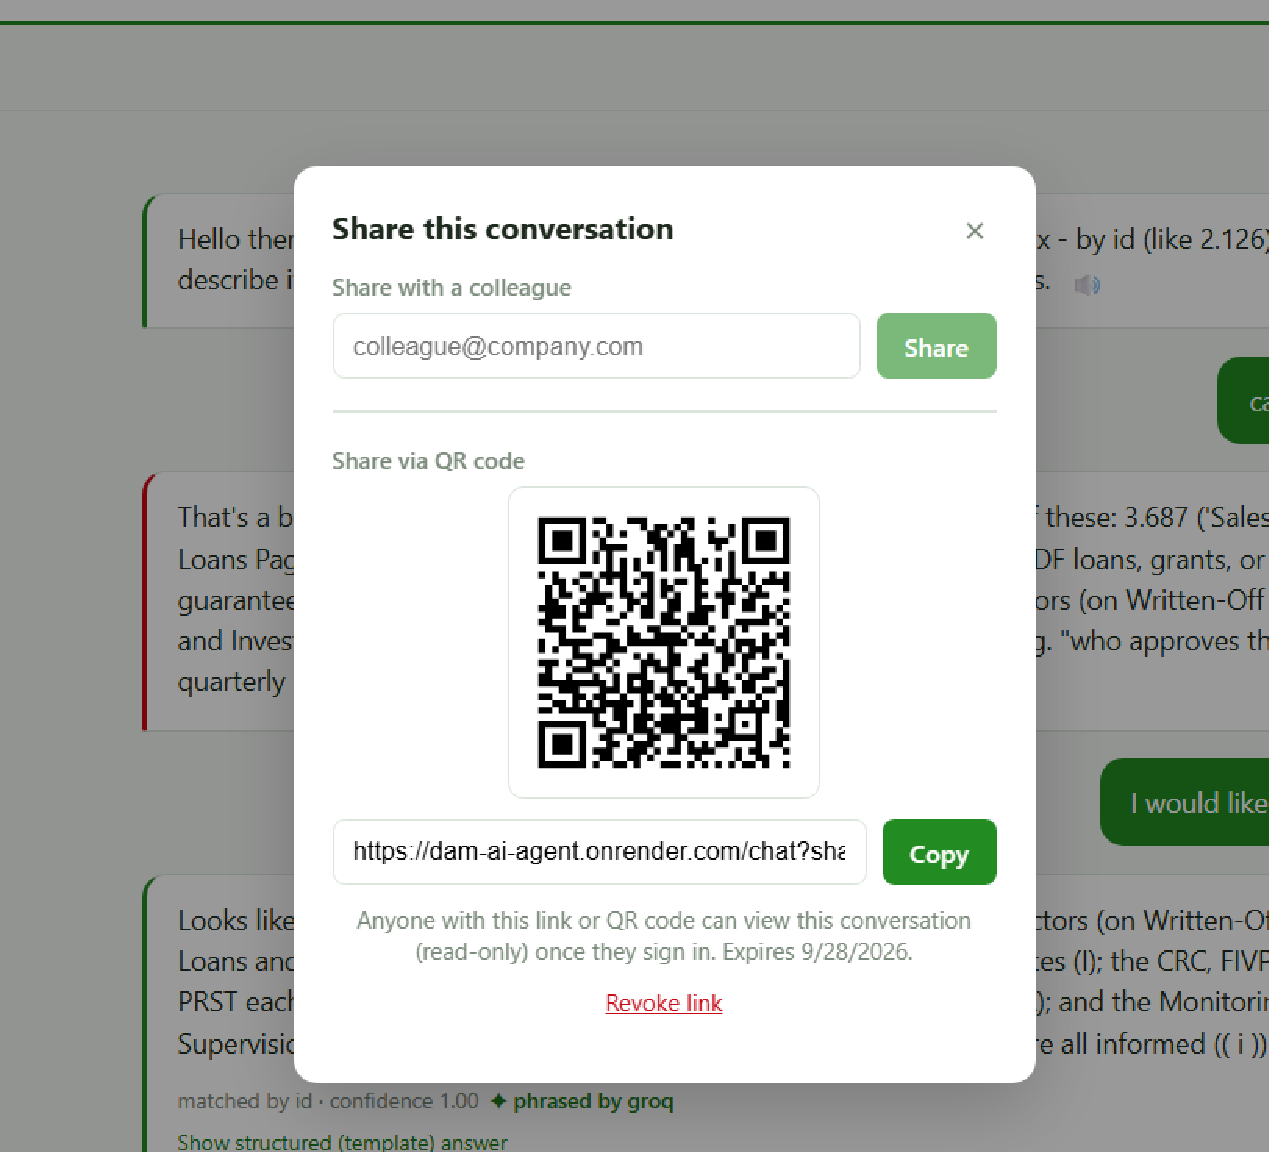
\includegraphics[width=0.7\textwidth]{figures/app-share-qr.pdf}
\caption{Sharing dialogue. A conversation may be shared with a named colleague or
through an expiring link rendered as a QR code, with the expiry date stated and revocation
available.}
\label{fig:appshare}
\end{figure}

Visiting a share link does not itself grant access. The recipient must be signed in, and
claiming the link invokes the same grant used by direct sharing, so the question of who
may view a conversation has exactly one answer in the code rather than two that must be
kept consistent. A link that has expired or been revoked is refused; the originating user
may revoke at any time before expiry.

\subsection{Real-Time Propagation}

A shared conversation is a live view rather than a copy. Messages added after sharing
appear to the recipient, which is the behaviour a colleague consulted mid-conversation
expects, and which a snapshot cannot provide.

Propagation uses two mechanisms together. The server maintains a per-account publish and
subscribe registry and pushes events to connected clients over a Server-Sent Events stream,
so a new message typically reaches a shared viewer within about a second. A thirty-second
poll runs alongside it. The redundancy is intentional: the stream is a long-lived
connection and free hosting tiers are not reliable custodians of those, so the poll bounds
how stale a view can become if the stream is dropped silently. One implementation detail
proved necessary in practice, namely that a background refresh is never permitted to
shorten a conversation already on screen, which otherwise allowed a poll completing
between a message being sent and its response arriving to momentarily erase it from the
sender's own view.

The registry is per-process, which is correct for the single-instance deployment described
later in this chapter and would require a shared broker to survive horizontal scaling.
This is recorded as a known boundary rather than left to be discovered.

Figure~\ref{fig:sharesse} traces one message through both channels, and the rule at the
bottom of the diagram is the one implementation detail mentioned above: a background
refresh may add messages to a shared view but may never remove or shorten what is already
displayed.

\begin{figure}[htbp]
\centering
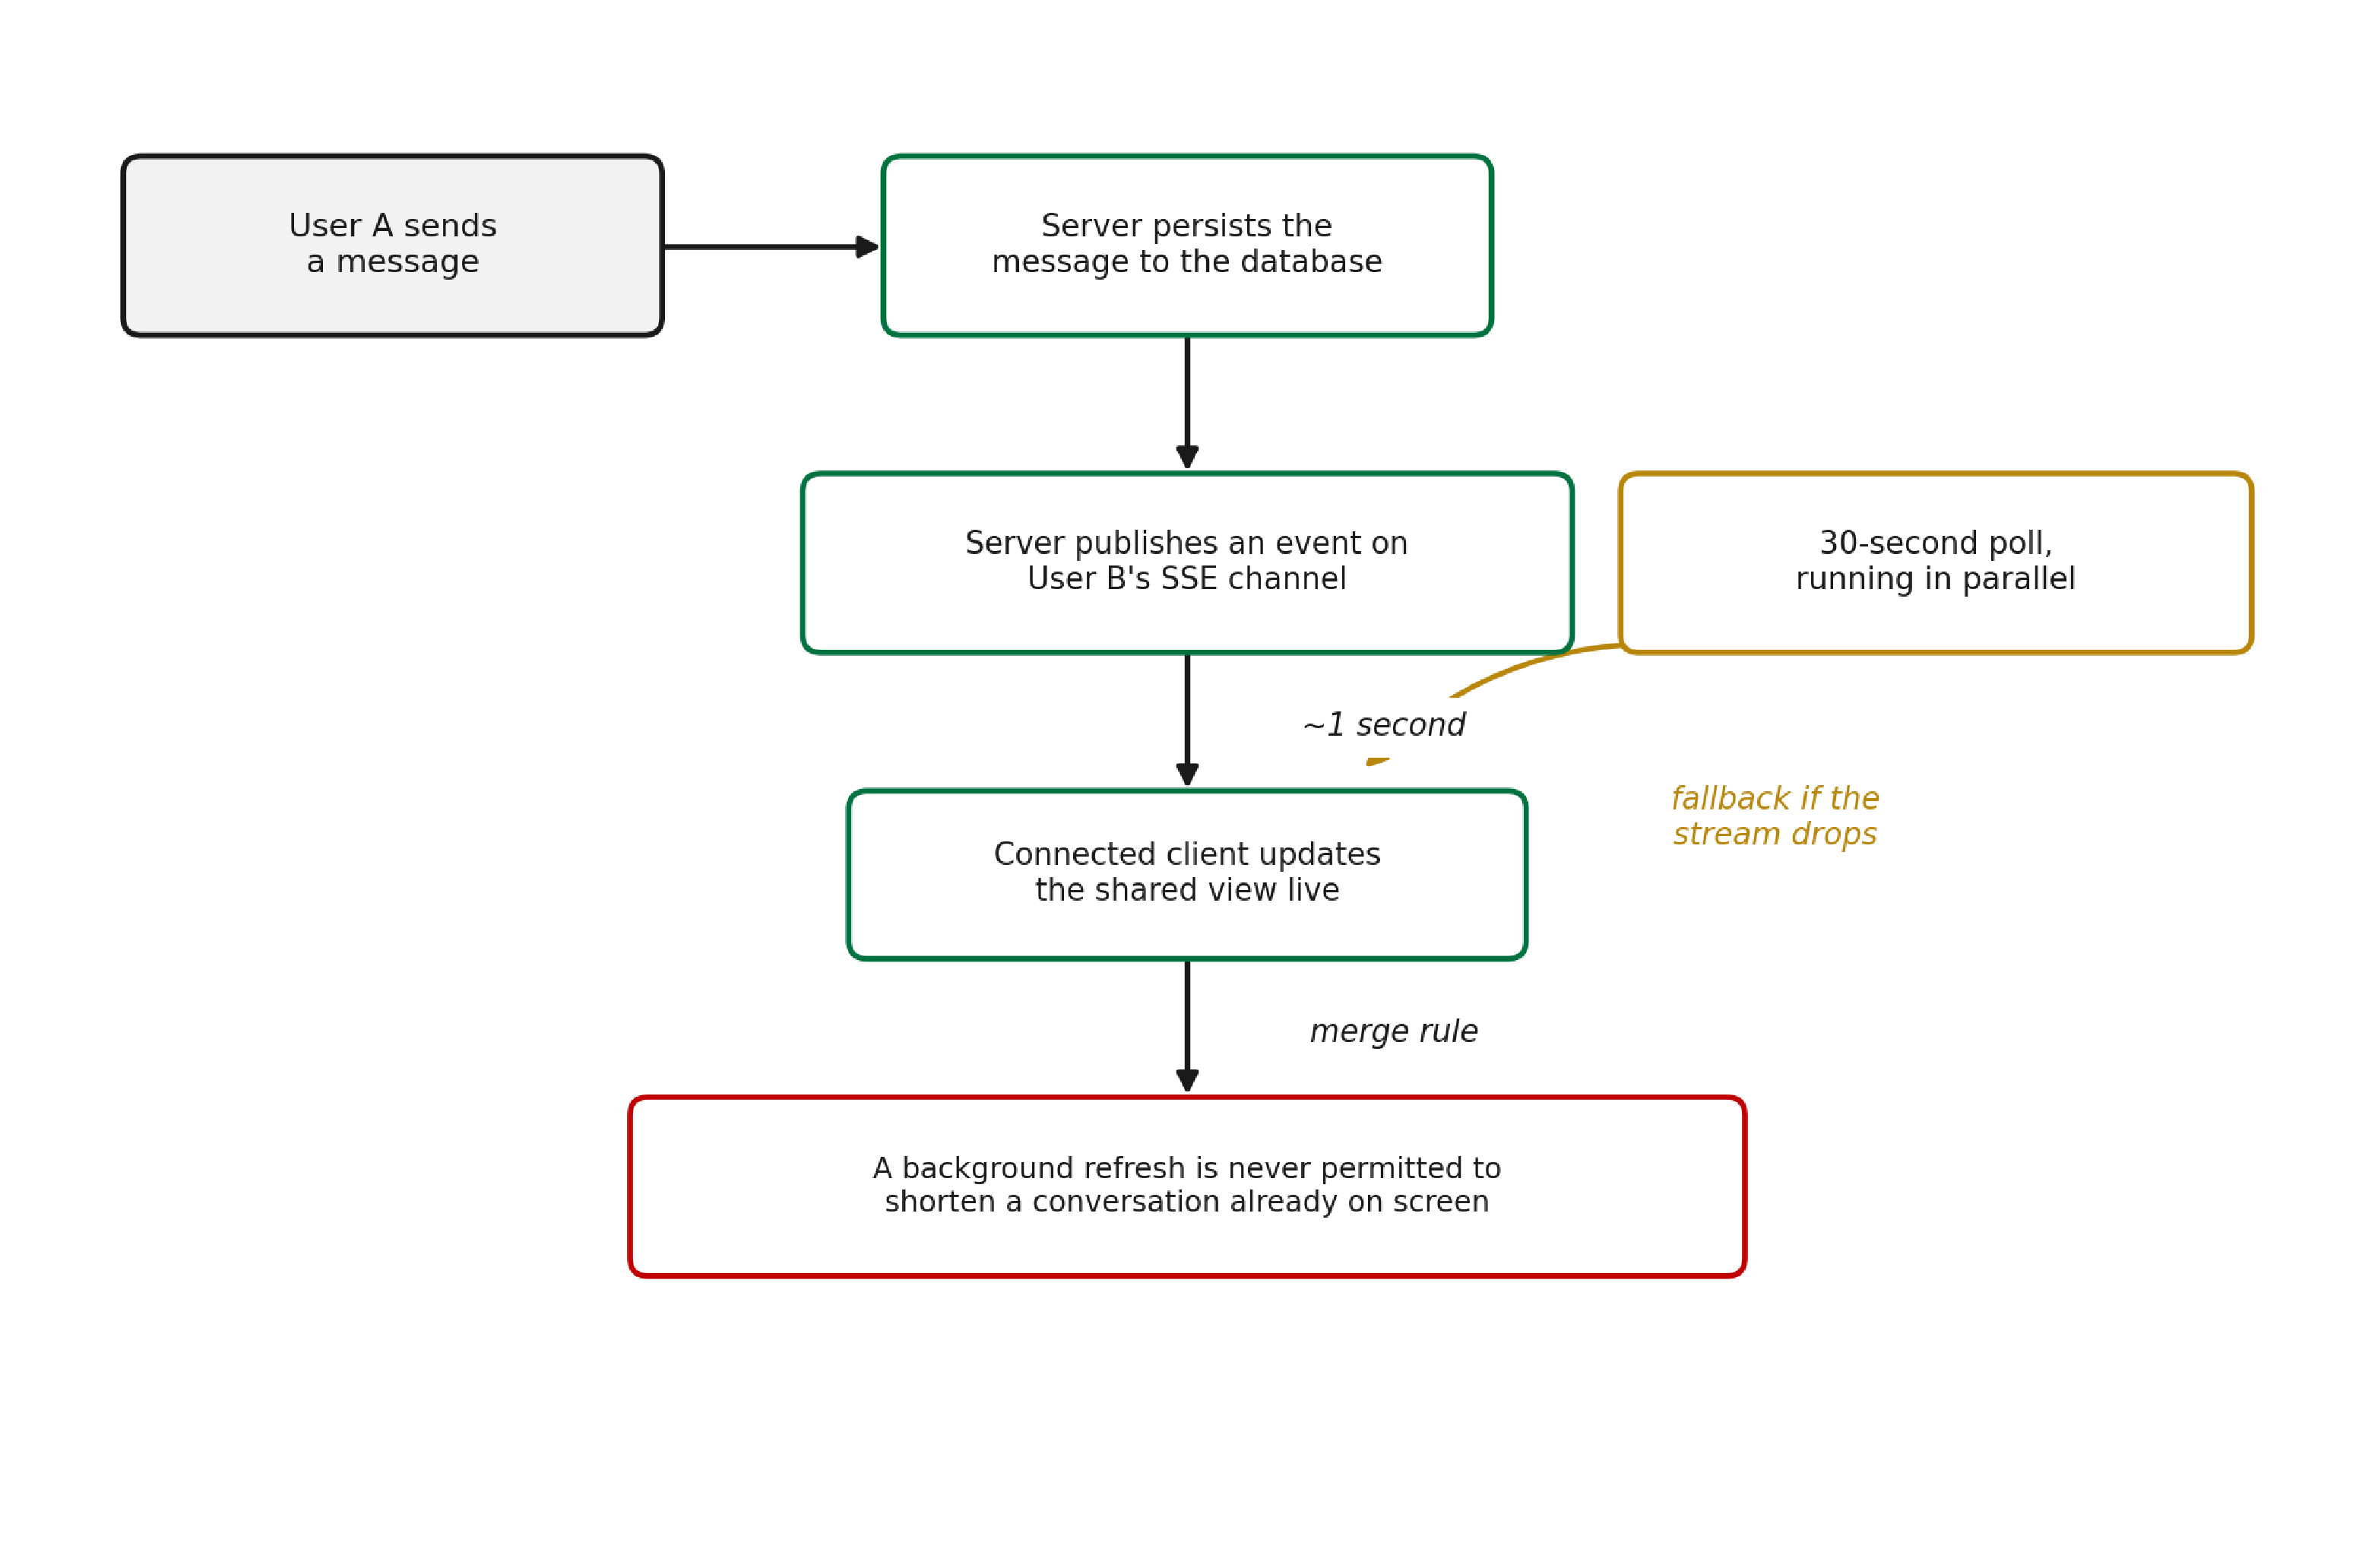
\includegraphics[width=0.86\textwidth]{figures/fig-sharesse.pdf}
\caption{Real-time propagation of a shared conversation. The Server-Sent Events stream
delivers a new message within about a second; the thirty-second poll is a fallback that
bounds staleness if the stream drops.}
\label{fig:sharesse}
\end{figure}

\section{Analytics Dashboard}

Everything up to this point has been about answering a question against one activity at a
time. The dashboard is the platform's one departure from that pattern: why it exists, how
its numbers are computed, which indicators earned a place on it, and which governance
indicators were specified but held back from the delivered release.

\subsection{Purpose}

Every other part of the platform answers questions about individual activities. The
dashboard does something different: it reports on the matrix as an object, and in doing so
exposes properties that no page-by-page reading reveals. A reader consulting the document
sees one activity at a time by construction. Questions such as how many roles hold
approval authority at all, how concentrated that authority is, or what proportion of the
document carries no responsibilities of its own, cannot be answered by reading. They can
be answered immediately once the same document is a graph.

Figure~\ref{fig:appdashboard} shows the delivered dashboard.

\begin{figure}[htbp]
\centering
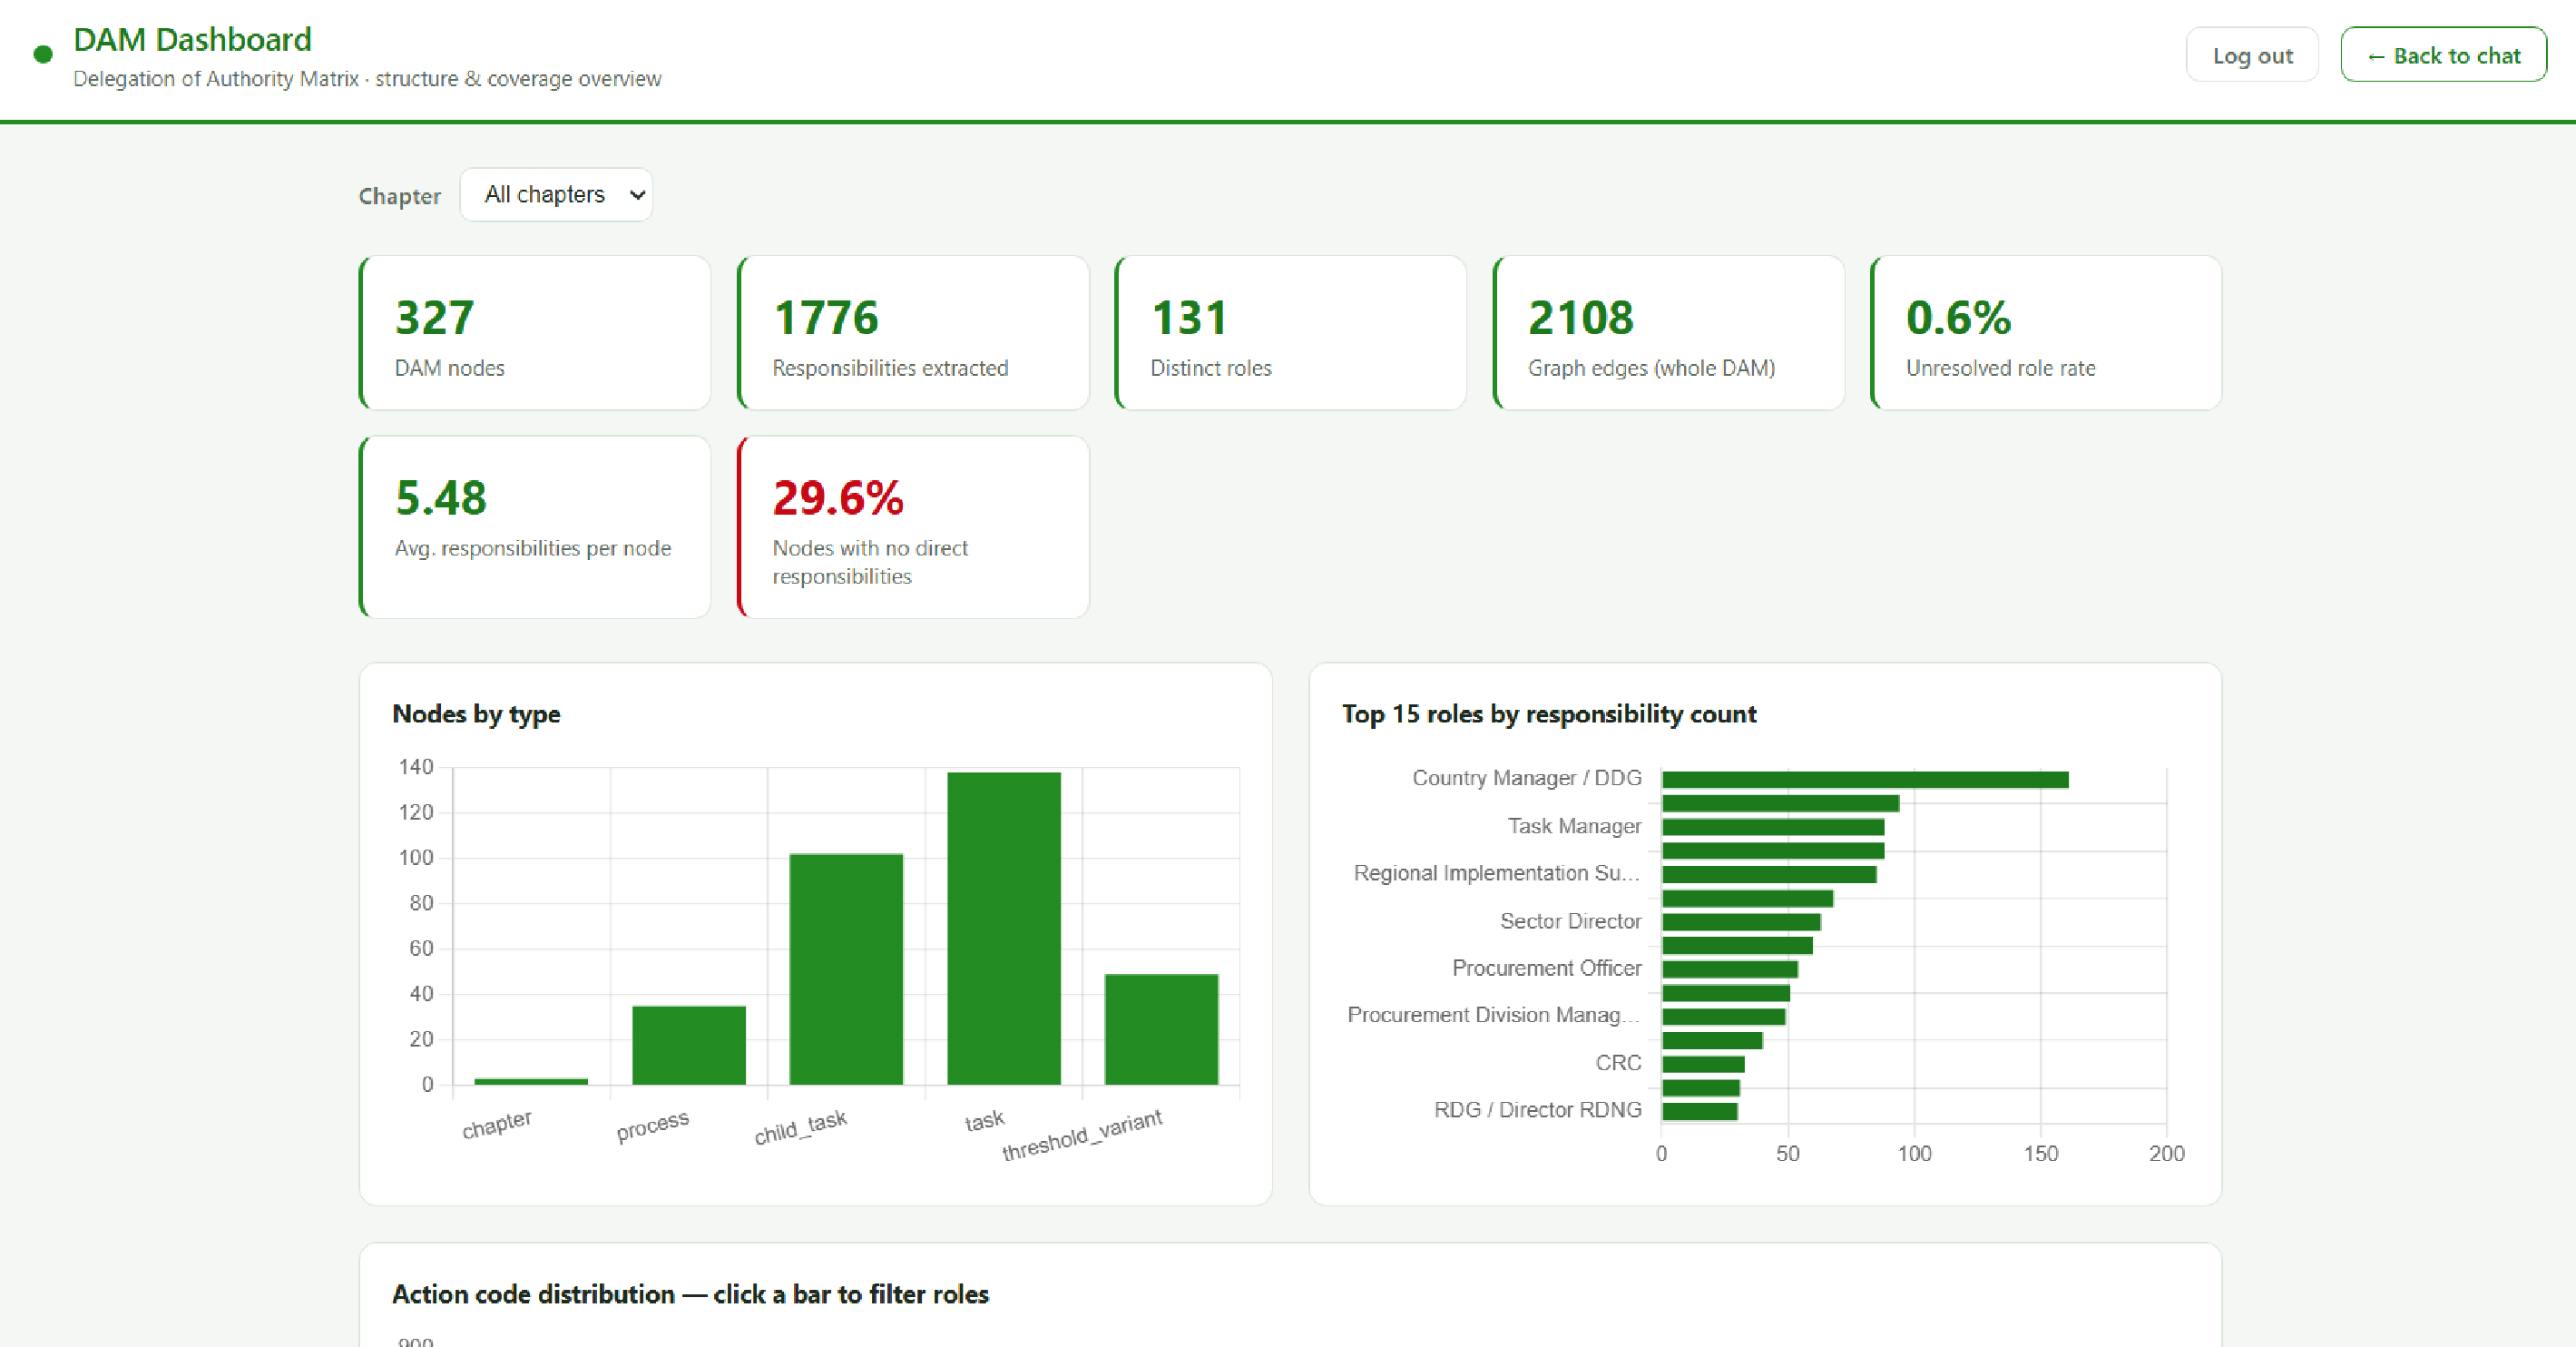
\includegraphics[width=0.98\textwidth]{figures/app-dashboard.pdf}
\caption{Analytics dashboard, showing headline indicators, the distribution of node
types, and the roles ranked by the number of responsibilities they carry.}
\label{fig:appdashboard}
\end{figure}

\subsection{Computation Model}

No statistic on the dashboard is stored. Every figure is computed at request time from the
node set and the graph already held in memory, which has one consequence worth stating
explicitly: the dashboard cannot drift out of agreement with the knowledge base, because
there is no second copy of the numbers that could become stale. A parser change that
alters the extraction is visible on the dashboard at the next request without any
recomputation step, and the cost of that guarantee is an aggregation over a few hundred
nodes, which is negligible.

The same computation is applied twice at different scopes. It runs once over every node in
the matrix, and once per chapter over that chapter's nodes, producing an identical
structure in both cases so that the client can render the whole-document view and a
single-chapter view through the same code path.

One quantity is deliberately not scoped by chapter. The graph edge total remains
whole-document, because responsibility and cross-reference edges routinely cross chapter
boundaries: the same role appears in several chapters, and a reference in one chapter
frequently points into another. A per-chapter edge count would require a defensible rule
for whether an edge leaving the chapter belongs to it, and any such rule would produce a
number more misleading than useful.

\subsection{How Indicators Were Chosen}

An indicator earns its place on a dashboard by changing what somebody does. That criterion
is easy to state and routinely ignored, and the usual result is a wall of counts that is
read once out of curiosity and never again. Each figure reported here was therefore required
to answer a specific question that somebody actually has, and the indicators fall into three
groups according to whose question it is.

The first group answers \emph{is the extraction still correct}, and its audience is whoever
maintains the pipeline. These are regression instruments: they exist because a parser change
can break a rule silently, producing a node set that is smaller or emptier or differently
distributed while every individual record still looks plausible. A sampled manual check does
not catch that. A number that moves does.

The second group answers \emph{what is in this document}, and its audience is a reader
trying to understand the matrix as an object rather than to look one activity up. A person
consulting the DAM sees one activity at a time by construction, which makes the shape of the
whole invisible to them however carefully they read.

The third group answers \emph{what does this document imply about the institution}, and its
audience is governance and audit. These are the indicators of Section~\ref{sec:govkpi}, and
they are specified rather than delivered.

The rest of this section takes the delivered indicators in turn and states, for each, what it
measures, why it was chosen, and what it turned out to show. Table~\ref{tab:dashkpi}
summarises them first.

\begin{longtable}{|p{0.27\textwidth}|p{0.11\textwidth}|p{0.14\textwidth}|p{0.36\textwidth}|}
\caption{Indicators computed by the delivered analytics dashboard.}\label{tab:dashkpi}\\
\hline
\rowcolor{myblue}\textcolor{white}{\textbf{Indicator}} & \textcolor{white}{\textbf{Value}} & \textcolor{white}{\textbf{Answers}} & \textcolor{white}{\textbf{Why it is reported}} \\
\hline
\endfirsthead
\hline
\rowcolor{myblue}\textcolor{white}{\textbf{Indicator}} & \textcolor{white}{\textbf{Value}} & \textcolor{white}{\textbf{Answers}} & \textcolor{white}{\textbf{Why it is reported}} \\
\hline
\endhead
DAM nodes & 327 & What is in it & Establishes the size of the extracted corpus and moves immediately if a parsing change drops records. \\ \hline
Responsibilities extracted & 1{,}776 & What is in it & The real size of the matrix. Activities are containers; obligations are the content. \\ \hline
Distinct roles & 131 & What is in it & Bounds how many organisational actors the delegation structure involves at all. \\ \hline
Graph edges & 2{,}108 & What is in it & Confirms the graph is connected rather than a set of isolated records. \\ \hline
Unresolved role rate & 0.6\% & Is it correct & The single most sensitive regression detector in the project. \\ \hline
Average responsibilities per node & 5.48 & What is in it & Procedural weight per activity, and a second regression signal. \\ \hline
Nodes with no direct responsibilities & 29.6\% & What is in it & Quantifies the redirect structure, and justifies a correctness requirement of the agent. \\ \hline
Node type distribution & --- & What is in it & Separates structural scaffolding from actionable activity. \\ \hline
Authority code distribution & --- & What is in it & Shows which obligations the institution actually uses, against the seventeen available. \\ \hline
Top roles by responsibility count & --- & What is in it & Ranks actors by load and exposes concentration. \\ \hline
\end{longtable}

\subsection{Correctness Indicators}

\paragraph{Unresolved role rate.} This measures the proportion of responsibilities whose
authority code was located in a cell but whose owning column could not be determined. It
exists because of how role attribution works: column headers in the source are printed
rotated through ninety degrees, are not recoverable as table headers, and must be
reconstructed by clustering header coordinates and matching each code to a column by
horizontal alignment. That reconstruction is the most fragile step in the pipeline, and when
it degrades it does so quietly, attaching obligations to no role at all rather than raising
an error.

It was added as a development instrument rather than as an analytical one. During the
geometric attribution work it was the number watched after every change, because a
modification that improved one page's clustering while breaking another's is invisible in a
sampled check and unmistakable here. Its present value of 0.6\% is the figure against which
the pipeline's adequacy is argued in Chapter~\ref{ch:pipeline}, and the ten or so
responsibilities behind that percentage are the residue of genuinely ambiguous layout rather
than a systematic fault.

\paragraph{Average responsibilities per node.} At 5.48, this serves a similar purpose from
the opposite direction. The unresolved rate catches codes that lost their role; this catches
codes that were never found. A parsing change that stops recognising a code in some layout
leaves every remaining record perfectly valid, so nothing fails, and the only symptom is that
activities become quietly thinner. Watching a mean rather than a total matters here, because
a total also moves when the processed scope changes, and a ratio does not.

\subsection{Structural Indicators}

\paragraph{Node and responsibility counts.} The corpus contains 327 records carrying 1,776
individual responsibilities. Reporting both is deliberate, because the second is the real
measure of the matrix and the first is routinely mistaken for it. An activity is a container;
the obligations attached to it are the content, and a document with few activities and many
obligations each is a very different thing from the reverse.

\paragraph{Node type distribution.} Records are counted by type, which separates the document
into structural scaffolding and actionable content. Chapters and processes exist to organise;
tasks, child tasks and threshold variants are what a user actually asks about. The
distribution is what makes it possible to say honestly how much of a 79-page document is
answerable material rather than hierarchy, and it also exposes the threshold-variant
population, which is the mechanism behind the near-identical-activities problem that motivated
the whole project in Chapter~\ref{ch:context}.

\paragraph{Authority code distribution.} Seventeen level-qualified notations are available in
the legend. This indicator shows which of them the institution actually uses and how often,
and the interesting result is the imbalance: the delegation structure leans heavily on a
small subset, while several codes appear rarely enough that their meaning is unlikely to be
familiar to most staff. That is an argument for the glossary expansion built into the agent,
grounded in a measurement rather than an assumption.

\paragraph{Distinct roles and the role ranking.} There are 131 distinct roles, and the top
fifteen by obligation count are ranked. The count bounds the size of the delegation structure;
the ranking exposes its shape. A long flat ranking would indicate authority spread evenly, and
a steep one indicates concentration in a handful of offices. The delivered ranking is visibly
steep, which is the observation that motivates the authority-concentration indicator specified
in Section~\ref{sec:govkpi}.

\paragraph{Graph edges.} The 2,108 edges confirm that the extraction produced a connected
structure rather than a pile of independent records. It is reported because the difference
between a list and a graph is the entire premise of the approach: if containment and reference
edges were absent, the cross-reference following of Chapter~\ref{ch:agent} would have nothing
to traverse.

\subsection{An Indicator That Changed the Design}

\paragraph{Records with no direct responsibilities.} At 29.6\%, this is the figure with the
largest consequence in the chapter, and it was not anticipated.

It counts responsibility-bearing records that carry no obligation of their own. Encountering
it for the first time, the natural reading is that something is broken: nearly a third of the
extracted activities appear empty. Checking those records against the printed pages showed the
extraction was correct and the document is simply built that way. Roughly three activities in
ten record nothing themselves and point to another activity instead.

That reframed a feature as a requirement. Cross-reference following had been treated as a
refinement, worth having for completeness. This measurement showed that a system without it
dead-ends on close to a third of the matrix, which is not a gap in polish but a failure on
routine questions. The redirect path described in Chapter~\ref{ch:agent} exists in the form it
does because this number was measured before the agent was finished.

It is also the clearest demonstration of why the dashboard was worth building. The fact was
always present in the document and always invisible to a reader, because a reader
encountering one empty activity concludes that this activity is unusual. Only the aggregate
reveals that it is the norm.

\subsection{Interactive Cross-Filtering}

The charts are linked rather than independent. Selecting an authority code in the
distribution chart filters the role ranking to the roles holding that specific authority,
which turns a static display into a means of asking a different class of question: not
which roles are busiest overall, but which roles hold approval authority specifically, or
which hold check-and-verify obligations. The two rankings are not the same, and the
difference between them is exactly the segregation-of-duties structure of the institution.

The cross-filter is computed server-side rather than derived in the browser, so that the
counting rules, in particular the exclusion of unresolved roles, are applied in one place
and cannot diverge between the ranking and the filtered ranking.

\subsection{Governance Indicators Derivable from the Graph}
\label{sec:govkpi}

The indicators above describe the document. A further family describes what the document
implies about the institution, and the graph supports all of them without requiring any
data source beyond the matrix itself. Table~\ref{tab:govkpi} specifies them.

These are specified rather than delivered. The dashboard as built reports the structural
indicators of Table~\ref{tab:dashkpi}; the governance family below is the designed
extension, defined here precisely enough to be implemented directly, and is not claimed as
a delivered capability.

\begin{longtable}{|p{0.28\textwidth}|p{0.58\textwidth}|}
\caption{Governance indicators derivable from the knowledge graph, specified as the designed extension to the dashboard.}\label{tab:govkpi}\\
\hline
\rowcolor{myblue}\textcolor{white}{\textbf{Indicator}} & \textcolor{white}{\textbf{Definition and interpretation}} \\
\hline
\endfirsthead
\hline
\rowcolor{myblue}\textcolor{white}{\textbf{Indicator}} & \textcolor{white}{\textbf{Definition and interpretation}} \\
\hline
\endhead
Authority concentration & Share of activities for which exactly one role holds approval authority. A high value identifies single points of failure, where one absence blocks a process. \\ \hline
Approval span per role & Number of activities each role approves. Ranks roles by the breadth of authority they carry and surfaces disproportionate concentration. \\ \hline
Segregation of duties & Share of activities where the initiating role differs from the approving role. A standard internal-control measure\citep{coso2013}, computed here directly from the matrix. \\ \hline
Verification coverage & Share of activities carrying at least one recorded check-and-verify obligation. Measures how much of the Bank's activity has a mandatory second pair of eyes. \\ \hline
Notification breadth & Mean number of informed parties per activity, with distribution. Indicates how widely decisions are communicated. \\ \hline
Threshold banding rate & Share of activities whose approver depends on a monetary band. Quantifies how far delegation is value-sensitive rather than flat. \\ \hline
Authority chain depth & Mean number of distinct roles involved in an activity across all authority types. A proxy for procedural weight. \\ \hline
Documentation completeness & Share of activities with no recorded responsibility of any kind, excluding structural containers. Flags gaps in the matrix itself. \\ \hline
Redirect dependency & Share of activities whose responsibilities are reachable only by following a cross-reference. Measures how much of the document is indirect. \\ \hline
Role redundancy & Share of activities with two or more roles able to approve. Read together with authority concentration, it separates resilience from ambiguity. \\ \hline
\end{longtable}

Two of these must be read together rather than separately. Authority concentration and
role redundancy are complementary, and either one alone supports the wrong conclusion: a
single approver is efficient but fragile, while multiple approvers are resilient but can
obscure who is actually accountable. Reported per chapter, the pair shows which pattern
each part of the institution has adopted.

Segregation of duties is the indicator most likely to interest an audit function. It is a
control principle the matrix already implements implicitly, in that the initiating and
approving roles for an activity are recorded separately, and which is currently measured
nowhere. Computing it requires no new data, only the graph that already exists, and it is
the strongest argument in this project for treating a governance document as structured
data rather than as a document.

\section{REST Interface}

Table~\ref{tab:api} lists the endpoints the backend exposes. The surface is deliberately
small, and one property of it is worth noting: the question endpoint is the only route
that reaches the agent, so every path through which an answer can be obtained passes
through the same verification.

\begin{longtable}{|p{0.47\textwidth}|p{0.09\textwidth}|p{0.38\textwidth}|}
\caption{REST API endpoints exposed by the backend.}\label{tab:api}\\
\hline
\rowcolor{myblue}\textcolor{white}{\textbf{Endpoint}} & \textcolor{white}{\textbf{Method}} & \textcolor{white}{\textbf{Purpose}} \\
\hline
\endfirsthead
\hline
\rowcolor{myblue}\textcolor{white}{\textbf{Endpoint}} & \textcolor{white}{\textbf{Method}} & \textcolor{white}{\textbf{Purpose}} \\
\hline
\endhead
\texttt{/api/auth/signup} & POST & Creates an account and returns a signed token. \\ \hline
\texttt{/api/auth/login} & POST & Exchanges credentials for a signed token. Rate-limited. \\ \hline
\texttt{/api/auth/me} & GET & Returns the authenticated account and its role. \\ \hline
\texttt{/api/auth/google/login}, \texttt{/callback} & GET & Federated sign-in through Google. \\ \hline
\texttt{/api/auth/microsoft/login}, \texttt{/callback} & GET & Federated sign-in through Microsoft. \\ \hline
\texttt{/api/ask} & POST & Core endpoint. Accepts a question, model mode, optional carried-over activity, target language, and optional attachment reference. Returns the answer, the deterministic answer, the resolved identifier, resolution method and score, and language and model metadata. \\ \hline
\texttt{/api/uploads} & POST & Stores an attachment against the calling account after type and size validation. \\ \hline
\texttt{/api/transcribe} & POST & Transcribes a dictated audio clip to text. \\ \hline
\texttt{/api/conversations} & GET, POST & Lists owned and shared conversations; creates a conversation. \\ \hline
\texttt{/api/conversations/\{id\}} & GET, DELETE & Retrieves or deletes a conversation. \\ \hline
\texttt{/api/conversations/\{id\}/messages} & POST & Appends an exchange with its provenance metadata. \\ \hline
\texttt{/api/conversations/\{id\}/attachments/\{key\}} & GET & Returns a short-lived presigned URL, subject to conversation-scoped permission. \\ \hline
\texttt{/api/conversations/\{id\}/share} & POST & Grants a named account read-only access. \\ \hline
\texttt{/api/conversations/\{id\}/share/\{user\}} & DELETE & Withdraws a previously granted access. \\ \hline
\texttt{/api/conversations/\{id\}/share-link} & POST, DELETE & Issues or revokes an expiring share link and its QR encoding. \\ \hline
\texttt{/api/conversations/shared/\{token\}/claim} & POST & Claims a share link for the signed-in account. \\ \hline
\texttt{/api/events} & GET & Server-Sent Events stream carrying conversation updates for the authenticated account. \\ \hline
\texttt{/api/dashboard/summary} & GET & Aggregate statistics, per-chapter breakdowns, and graph totals. Administrator only. \\ \hline
\texttt{/api/llm/config} & GET & Reports the model each mode would currently use. \\ \hline
\texttt{/api/health} & GET & Liveness check used by the platform and the status indicator. Reports nodes loaded. \\ \hline
\end{longtable}

\section{Testing and Validation}

The system carries 375 automated tests across 33 files. The count matters less than their
provenance: these are not tests written to reach a coverage target. Almost every one exists
because a specific defect was found, and the test was written to pin the corrected
behaviour so that it could not silently return. Table~\ref{tab:tests} gives the
distribution.

\begin{longtable}{|p{0.34\textwidth}|p{0.09\textwidth}|p{0.45\textwidth}|}
\caption{Breakdown of the automated test suite.}\label{tab:tests}\\
\hline
\rowcolor{myblue}\textcolor{white}{\textbf{Area}} & \textcolor{white}{\textbf{Tests}} & \textcolor{white}{\textbf{Coverage}} \\
\hline
\endfirsthead
\hline
\rowcolor{myblue}\textcolor{white}{\textbf{Area}} & \textcolor{white}{\textbf{Tests}} & \textcolor{white}{\textbf{Coverage}} \\
\hline
\endhead
Extraction and parsing & 42 & Task boundary detection, split-row merging, rotated header extraction, title recovery, reference and footnote handling, glossary parsing \\ \hline
Node and graph construction & 16 & Node assembly, hierarchy correctness, graph edges, lossless caching \\ \hline
Retrieval and agent behaviour & 63 & Identifier fast path, free-text resolution, typo tolerance, small talk, authority codes, glossary lookup, answer orchestration \\ \hline
Language model layer & 59 & Provider mocking and failure handling, verification-step correctness, translation, tone classification \\ \hline
Attachments and storage & 37 & Text extraction per format, vision routing, object storage, upload validation, attachment question answering \\ \hline
Authentication and accounts & 21 & Password hashing, token issuance and expiry, rate limiting, federated sign-in \\ \hline
Conversations and sharing & 33 & Persistence, direct shares, share links, claim, expiry, revocation \\ \hline
Real-time events & 6 & Publish and subscribe registry, fan-out, de-duplication \\ \hline
API and error handling & 42 & End-to-end route behaviour, attachment branch authorisation, unhandled-error contract \\ \hline
Dashboard and client & 31 & Dashboard metrics, chapter scoping, structural checks on the web client source \\ \hline
\textbf{Total} & \textbf{375} & \textbf{across 33 files} \\ \hline
\end{longtable}

Automated testing was not the only form of verification. Individual records were checked
against the printed pages they were extracted from, which is the only way to detect an
answer that is plausible and wrong, and the running system was exercised with real
questions before each significant change.

Two defects found during a late verification pass are reported here rather than removed. In
one pair of records a column header was attributed as though it were a role, producing a
responsibility held by a role name that does not exist in the organisation. In the same two
records, two adjacent footnote digits were fused into a single number, yielding a footnote
reference that matches no actual footnote. Both are localised to those records, both are
visible in a live answer, and both are scheduled for correction alongside the footnote
extraction work described in the general conclusion. They are stated because a report that
describes only the defects that were fixed gives a misleading account of the state of the
system.

\section{Deployment}
\label{sec:deployment}

The application is containerised\citep{docker_docs} through a multi-stage build that
compiles the web client and packages the result with the Python service, so the image that
runs in production is the image that was built and tested rather than an environment
assembled at deploy time. A companion composition adds a local model container for offline
operation; the hosted provider needs no container, being reached over the network.

Deployment targets a free hosting tier\citep{render_docs} with automatic redeployment on
every change to the main branch. The first attempt failed, and the failure is instructive.
The service parsed the source PDF at startup, exceeded the platform's memory ceiling, and
was terminated before it ever served a request. The resolution was to move parsing to
build time and ship the serialised node set, reducing startup to a file load. This brought
both memory use and startup time within the platform's limits, and it is the direct reason
the knowledge base is an immutable build artefact rather than something constructed at
runtime, as described at the start of this chapter. The constraint produced the
architecture.

\section*{Conclusion}
\addcontentsline{toc}{section}{Conclusion}

This chapter has presented the platform delivered around the agent. Authentication
establishes ownership; ownership makes persistence meaningful; persistence makes sharing
possible; and sharing, once conversations are live objects rather than snapshots,
required a real-time channel. Each capability rests on the one before it, and none of them
required modifying the retrieval or generation components, which is the practical payoff
of the architectural separation argued for in Chapter~\ref{ch:agent}.

The dashboard is the part of the system that does something the original document cannot.
Reading the matrix answers questions about one activity; querying the graph answers
questions about the institution. The structural indicators delivered here are modest in
number, but two of them, the unresolved role rate and the proportion of records with no
direct responsibilities, turned out to serve as both engineering instruments and
analytical findings, the second quantifying a redirect structure that directly justifies a
correctness requirement of the agent.

The system is deployed, reachable, and covered by 375 automated tests. It is also
incomplete in ways this chapter has stated rather than concealed: localisation stops at
the conversation interface, the governance indicators are specified but not implemented,
and two extraction defects remain live. The general conclusion which follows sets these
against what the project set out to do.

\chapter*{General Conclusion}
\addcontentsline{toc}{chapter}{General Conclusion}
\markboth{General Conclusion}{General Conclusion}

This work started with a document that has a problem with how it answers an important question: it's not a problem with the question itself, it's a problem in its form, and that form makes it difficult to retrieve. The DAM says who is authorized to approve, check, review, initiate, and be informed about all of the Bank's activities, and it is written within wide tables, with sideways headers, and a compact notation which cannot be easily looked up by hand or processed by computer.

What is constructed in response is a system which looks at the question of what facts are, and the question of how to say them. It was successfully parsed into 327 valid records with 1,776 responsibility entries, and converted to a graph of 459 nodes and 2,108 edges, with less than one percent of the responsibility entries not yet resolved. The answers are built from records in that graph; the answers are rewritten, to natural sentences, by a language model under a verification step which does not accept any rewriting that omits or changes a fact; questions are resolved to activities by an exact identifier path and a lexical search layer. Around that core is an authenticated platform with voice input, an explicit trust boundary for document attachment, conversations that can be shared read-only with a colleague and stay live as they are extended, a conversation interface localised into five languages, and an analytics dashboard that reports the structure and extraction quality of the matrix itself.

The following three points seem to be conclusions that can be drawn from this work.

The first is related to the extraction of documents. All of the significant problems that arose during this project yielded seemingly plausible output that would not have been detected by simply verifying that the program ran without error. They were discovered by cross-referencing the extracted information with the pages in which it was found. If the document is visual, then, that comparison is not a nice-to-have for quality assurance, but it is the only way.

The second relates to language models in factual contexts. Asking a model not to make up facts is not a given. It had to be made a property of the system, which involved a mechanical check of the model's output, against the facts it was provided with. It is easy to check, inexpensive, and it is why there is any use for a generative component in a compliance context. It's the same idea as what's been described in Chapter~5 about logging how often that check fires: a safety property that's not measured in production is an assumption; it is not a guarantee.

The third is about refusal. The third is about refusal. The ability of the system to state that an identifier does not exist, or that a question falls outside the document it holds, rather than returning the nearest plausible match, is what makes the rest of its answers worth trusting.

\section*{Limitations}

The DAM was processed from a document of more than two hundred and fifty pages, and each chapter of the DAM is processed. The other chapters follow the same format, but that is yet to be proven.

Footnote handling is inadequate, and the most significant inadequacy. The responsibility numbers are extracted and linked to the footnote, and there are 113 such occurrences of responsibility numbers out of 1,776 of responsibility entries, but the text at the foot of the page is not parsed. The system can thus say that a qualification applies to a responsibility but fail to say what that qualification is. Because some footnotes in this document have conditions attached to them, such as delegation ceilings and prior approval requirements, an answer that names an approver but doesn't state the conditions attached to the approval is accurate but might be misleading. The two related extraction defects 1.116.1 and 1.116.2, the column header labeled as a role, and two footnote digits that are combined are all in the same part of the pipeline.

This was intentionally not started before a question, which the schema itself raises: is it the beginning of each chapter or of each process that footnote numbering starts again? The analysis of the extracted references shows that each reference appears at chapter level, as eleven different footnote numbers are repeated in two or more chapters, and there is no restart of numbers in each chapter. It is still not known for certain from two printed pages, however, which requires a parser to be built upon, something the rest of this project did.

Retrieval is lexical—that is, if the question is strictly in the terminology of the document, it will not be a successful retrieval. The system represents one version of one document and there is no way to determine whether the underlying DAM has been updated, which is more of an operational than theoretical concern in an institutional environment.

\section*{Perspectives}

The most straight-forward continuation is to finish the footnote extraction (which fixes the two known footnote extraction flaws at the same time), and then to process the rest of the chapters, testing that the parsing rules hold up as expected.

In addition, it would be desirable to have a hybrid retrieval layer that integrates the existing lexical matching with a semantic component to better resolve queries that use out-of-vocabulary terms, while maintaining the existing verification step unchanged. If a versioning mechanism can compare a new issue of the DAM with the existing knowledge base, and report on any changes, then a static reference becomes a maintainable one.

The direction of analytics is the most open. The governance indicators in Chapter~5 are indicators of properties of the matrix that no one is currently measuring, and and implementing them requires no data beyond the graph that already exists. Recording consultation activity would open a second direction, since a log of which activities are actually asked about would turn unanswered questions into a prioritised work list for extracting the remaining chapters. If the analysis of the graph could be extended to questions that the printed document cannot readily answer, such as where authority is located, in which roles there are unexpectedly many people in approval paths, or where one point of failure, such as an approval path, has more than one person in a chain of obligations, then it would be a governance instrument, and not merely a lookup gadget.

% References are split into a Bibliography (academic works, standards,
% frameworks) and a Webography (documentation and web resources), both
% written out in Bibliography.tex with continuous numbering.
% =====================================================================
%  REFERENCES, IN TWO PARTS
%  Bibliography : peer-reviewed articles, books, conference papers, a
%                 doctoral thesis, formal standards and published
%                 frameworks.
%  Webography   : documentation sites, software project pages and
%                 web products. Access dates follow the stage of the
%                 project at which each source was actually used.
%
%  Written out by hand rather than generated by BibTeX so that the two
%  lists render as separate sections with continuous numbering, which
%  no BibTeX style does on its own.
% =====================================================================

\renewcommand{\bibname}{Bibliography}

\begin{thebibliography}{99}
\addcontentsline{toc}{chapter}{Bibliography}

\bibitem{salton1988}
G.~Salton and C.~Buckley.
\newblock Term-weighting approaches in automatic text retrieval.
\newblock \emph{Information Processing \& Management}, 24(5):513--523, 1988.

\bibitem{manning2008ir}
C.~D. Manning, P.~Raghavan, and H.~Sch{\"u}tze.
\newblock \emph{Introduction to Information Retrieval}.
\newblock Cambridge University Press, Cambridge, U.K., 2008.

\bibitem{lewis2020rag}
P.~Lewis et~al.
\newblock Retrieval-augmented generation for knowledge-intensive {NLP} tasks.
\newblock In \emph{Advances in Neural Information Processing Systems (NeurIPS)},
  volume~33, pages 9459--9474, 2020.

\bibitem{ji2023hallucination}
Z.~Ji et~al.
\newblock Survey of hallucination in natural language generation.
\newblock \emph{ACM Computing Surveys}, 55(12):article 248, March 2023.

\bibitem{hogan2021kg}
A.~Hogan et~al.
\newblock Knowledge graphs.
\newblock \emph{ACM Computing Surveys}, 54(4):article 71, July 2021.

\bibitem{provos1999bcrypt}
N.~Provos and D.~Mazi{\`e}res.
\newblock A future-adaptable password scheme.
\newblock In \emph{Proceedings of the USENIX Annual Technical Conference}, 1999.

\bibitem{fielding2000rest}
R.~T. Fielding.
\newblock \emph{Architectural Styles and the Design of Network-based Software
  Architectures}.
\newblock PhD thesis, University of California, Irvine, 2000.

\bibitem{pedregosa2011sklearn}
F.~Pedregosa et~al.
\newblock Scikit-learn: Machine learning in {P}ython.
\newblock \emph{Journal of Machine Learning Research}, 12:2825--2830, 2011.

\bibitem{hagberg2008networkx}
A.~Hagberg, D.~Schult, and P.~Swart.
\newblock Exploring network structure, dynamics, and function using {NetworkX}.
\newblock In \emph{Proceedings of the 7th Python in Science Conference (SciPy)},
  pages 11--15, 2008.

\bibitem{seabold2010statsmodels}
S.~Seabold and J.~Perktold.
\newblock Statsmodels: Econometric and statistical modeling with {P}ython.
\newblock In \emph{Proceedings of the 9th Python in Science Conference (SciPy)},
  pages 92--96, 2010.

\bibitem{rfc7519}
M.~Jones, J.~Bradley, and N.~Sakimura.
\newblock {JSON} Web Token ({JWT}).
\newblock IETF RFC 7519, May 2015.

\bibitem{rfc7515}
M.~Jones, J.~Bradley, and N.~Sakimura.
\newblock {JSON} Web Signature ({JWS}).
\newblock IETF RFC 7515, May 2015.

\bibitem{coso2013}
Committee of Sponsoring Organizations of the Treadway Commission (COSO).
\newblock \emph{Internal Control --- Integrated Framework}.
\newblock 2013.

\bibitem{afdb_dam}
African Development Bank.
\newblock \emph{Delegation of Authority Matrix}.
\newblock Internal institutional document; primary data source of this study.

\end{thebibliography}

% ---------------------------------------------------------------------

\renewcommand{\bibname}{Webography}

\begin{thebibliography}{99}
\addcontentsline{toc}{chapter}{Webography}
\setcounter{NAT@ctr}{14}

\bibitem{polytechintl}
Polytech Intl --- \'Ecole Polytechnique Internationale Priv\'ee de Tunis.
\newblock \url{https://pi.tn/en/}
\newblock Accessed February 2026.

\bibitem{afdb}
African Development Bank Group.
\newblock About the African Development Bank Group.
\newblock \url{https://www.afdb.org}
\newblock Accessed February 2026.

\bibitem{chatpdf}
ChatPDF.
\newblock \url{https://www.chatpdf.com}
\newblock Accessed March 2026.

\bibitem{notebooklm}
Google.
\newblock NotebookLM.
\newblock \url{https://notebooklm.google}
\newblock Accessed March 2026.

\bibitem{ms365copilot}
Microsoft.
\newblock Microsoft 365 Copilot.
\newblock \url{https://www.microsoft.com/microsoft-365/copilot}
\newblock Accessed March 2026.

\bibitem{pdfplumber}
J.~Singer-Vine.
\newblock pdfplumber [software].
\newblock \url{https://github.com/jsvine/pdfplumber}
\newblock Accessed March 2026.

\bibitem{pydantic_docs}
Pydantic developers.
\newblock Pydantic documentation.
\newblock \url{https://docs.pydantic.dev}
\newblock Accessed April 2026.

\bibitem{groq}
Groq Inc.
\newblock Groq {API} documentation.
\newblock \url{https://groq.com}
\newblock Accessed May 2026.

\bibitem{ollama}
Ollama.
\newblock Ollama documentation.
\newblock \url{https://ollama.com}
\newblock Accessed May 2026.

\bibitem{fastapi_docs}
S.~Ram{\'i}rez.
\newblock {FastAPI} documentation.
\newblock \url{https://fastapi.tiangolo.com}
\newblock Accessed June 2026.

\bibitem{react_docs}
Meta Open Source.
\newblock React documentation.
\newblock \url{https://react.dev}
\newblock Accessed June 2026.

\bibitem{vite_docs}
Vite contributors.
\newblock Vite documentation.
\newblock \url{https://vitejs.dev}
\newblock Accessed June 2026.

\bibitem{webspeech_api}
W3C Community Group.
\newblock Web Speech {API}.
\newblock \url{https://wicg.github.io/speech-api/}
\newblock Accessed July 2026.

\bibitem{python_jose_docs}
python-jose contributors.
\newblock python-jose documentation.
\newblock \url{https://github.com/mpdavis/python-jose}
\newblock Accessed July 2026.

\bibitem{passlib_docs}
passlib contributors.
\newblock Passlib documentation.
\newblock \url{https://passlib.readthedocs.io}
\newblock Accessed July 2026.

\bibitem{owasp_cheatsheets}
OWASP Foundation.
\newblock {JSON} Web Token and Session Management cheat sheets.
\newblock OWASP Cheat Sheet Series, \url{https://cheatsheetseries.owasp.org}
\newblock Accessed August 2026.

\bibitem{reportlab_docs}
ReportLab.
\newblock {ReportLab} {PDF} library documentation.
\newblock \url{https://www.reportlab.com}
\newblock Accessed August 2026.

\bibitem{docker_docs}
Docker Inc.
\newblock Docker documentation.
\newblock \url{https://docs.docker.com}
\newblock Accessed August 2026.

\bibitem{render_docs}
Render Services, Inc.
\newblock Render documentation.
\newblock \url{https://render.com/docs}
\newblock Accessed September 2026.

\end{thebibliography}


\end{document}